\documentclass[]{book}
\usepackage{lmodern}
\usepackage{amssymb,amsmath}
\usepackage{ifxetex,ifluatex}
\usepackage{fixltx2e} % provides \textsubscript
\ifnum 0\ifxetex 1\fi\ifluatex 1\fi=0 % if pdftex
  \usepackage[T1]{fontenc}
  \usepackage[utf8]{inputenc}
\else % if luatex or xelatex
  \ifxetex
    \usepackage{mathspec}
  \else
    \usepackage{fontspec}
  \fi
  \defaultfontfeatures{Ligatures=TeX,Scale=MatchLowercase}
\fi
% use upquote if available, for straight quotes in verbatim environments
\IfFileExists{upquote.sty}{\usepackage{upquote}}{}
% use microtype if available
\IfFileExists{microtype.sty}{%
\usepackage{microtype}
\UseMicrotypeSet[protrusion]{basicmath} % disable protrusion for tt fonts
}{}
\usepackage[margin=1in]{geometry}
\usepackage{hyperref}
\hypersetup{unicode=true,
            pdftitle={AFAM Toolkit Guidance Document},
            pdfauthor={Gavin McDonald},
            pdfborder={0 0 0},
            breaklinks=true}
\urlstyle{same}  % don't use monospace font for urls
\usepackage{natbib}
\bibliographystyle{apalike}
\usepackage{color}
\usepackage{fancyvrb}
\newcommand{\VerbBar}{|}
\newcommand{\VERB}{\Verb[commandchars=\\\{\}]}
\DefineVerbatimEnvironment{Highlighting}{Verbatim}{commandchars=\\\{\}}
% Add ',fontsize=\small' for more characters per line
\usepackage{framed}
\definecolor{shadecolor}{RGB}{248,248,248}
\newenvironment{Shaded}{\begin{snugshade}}{\end{snugshade}}
\newcommand{\KeywordTok}[1]{\textcolor[rgb]{0.13,0.29,0.53}{\textbf{#1}}}
\newcommand{\DataTypeTok}[1]{\textcolor[rgb]{0.13,0.29,0.53}{#1}}
\newcommand{\DecValTok}[1]{\textcolor[rgb]{0.00,0.00,0.81}{#1}}
\newcommand{\BaseNTok}[1]{\textcolor[rgb]{0.00,0.00,0.81}{#1}}
\newcommand{\FloatTok}[1]{\textcolor[rgb]{0.00,0.00,0.81}{#1}}
\newcommand{\ConstantTok}[1]{\textcolor[rgb]{0.00,0.00,0.00}{#1}}
\newcommand{\CharTok}[1]{\textcolor[rgb]{0.31,0.60,0.02}{#1}}
\newcommand{\SpecialCharTok}[1]{\textcolor[rgb]{0.00,0.00,0.00}{#1}}
\newcommand{\StringTok}[1]{\textcolor[rgb]{0.31,0.60,0.02}{#1}}
\newcommand{\VerbatimStringTok}[1]{\textcolor[rgb]{0.31,0.60,0.02}{#1}}
\newcommand{\SpecialStringTok}[1]{\textcolor[rgb]{0.31,0.60,0.02}{#1}}
\newcommand{\ImportTok}[1]{#1}
\newcommand{\CommentTok}[1]{\textcolor[rgb]{0.56,0.35,0.01}{\textit{#1}}}
\newcommand{\DocumentationTok}[1]{\textcolor[rgb]{0.56,0.35,0.01}{\textbf{\textit{#1}}}}
\newcommand{\AnnotationTok}[1]{\textcolor[rgb]{0.56,0.35,0.01}{\textbf{\textit{#1}}}}
\newcommand{\CommentVarTok}[1]{\textcolor[rgb]{0.56,0.35,0.01}{\textbf{\textit{#1}}}}
\newcommand{\OtherTok}[1]{\textcolor[rgb]{0.56,0.35,0.01}{#1}}
\newcommand{\FunctionTok}[1]{\textcolor[rgb]{0.00,0.00,0.00}{#1}}
\newcommand{\VariableTok}[1]{\textcolor[rgb]{0.00,0.00,0.00}{#1}}
\newcommand{\ControlFlowTok}[1]{\textcolor[rgb]{0.13,0.29,0.53}{\textbf{#1}}}
\newcommand{\OperatorTok}[1]{\textcolor[rgb]{0.81,0.36,0.00}{\textbf{#1}}}
\newcommand{\BuiltInTok}[1]{#1}
\newcommand{\ExtensionTok}[1]{#1}
\newcommand{\PreprocessorTok}[1]{\textcolor[rgb]{0.56,0.35,0.01}{\textit{#1}}}
\newcommand{\AttributeTok}[1]{\textcolor[rgb]{0.77,0.63,0.00}{#1}}
\newcommand{\RegionMarkerTok}[1]{#1}
\newcommand{\InformationTok}[1]{\textcolor[rgb]{0.56,0.35,0.01}{\textbf{\textit{#1}}}}
\newcommand{\WarningTok}[1]{\textcolor[rgb]{0.56,0.35,0.01}{\textbf{\textit{#1}}}}
\newcommand{\AlertTok}[1]{\textcolor[rgb]{0.94,0.16,0.16}{#1}}
\newcommand{\ErrorTok}[1]{\textcolor[rgb]{0.64,0.00,0.00}{\textbf{#1}}}
\newcommand{\NormalTok}[1]{#1}
\usepackage{longtable,booktabs}
\usepackage{graphicx,grffile}
\makeatletter
\def\maxwidth{\ifdim\Gin@nat@width>\linewidth\linewidth\else\Gin@nat@width\fi}
\def\maxheight{\ifdim\Gin@nat@height>\textheight\textheight\else\Gin@nat@height\fi}
\makeatother
% Scale images if necessary, so that they will not overflow the page
% margins by default, and it is still possible to overwrite the defaults
% using explicit options in \includegraphics[width, height, ...]{}
\setkeys{Gin}{width=\maxwidth,height=\maxheight,keepaspectratio}
\IfFileExists{parskip.sty}{%
\usepackage{parskip}
}{% else
\setlength{\parindent}{0pt}
\setlength{\parskip}{6pt plus 2pt minus 1pt}
}
\setlength{\emergencystretch}{3em}  % prevent overfull lines
\providecommand{\tightlist}{%
  \setlength{\itemsep}{0pt}\setlength{\parskip}{0pt}}
\setcounter{secnumdepth}{5}
% Redefines (sub)paragraphs to behave more like sections
\ifx\paragraph\undefined\else
\let\oldparagraph\paragraph
\renewcommand{\paragraph}[1]{\oldparagraph{#1}\mbox{}}
\fi
\ifx\subparagraph\undefined\else
\let\oldsubparagraph\subparagraph
\renewcommand{\subparagraph}[1]{\oldsubparagraph{#1}\mbox{}}
\fi

%%% Use protect on footnotes to avoid problems with footnotes in titles
\let\rmarkdownfootnote\footnote%
\def\footnote{\protect\rmarkdownfootnote}

%%% Change title format to be more compact
\usepackage{titling}

% Create subtitle command for use in maketitle
\newcommand{\subtitle}[1]{
  \posttitle{
    \begin{center}\large#1\end{center}
    }
}

\setlength{\droptitle}{-2em}
  \title{AFAM Toolkit Guidance Document}
  \pretitle{\vspace{\droptitle}\centering\huge}
  \posttitle{\par}
  \author{Gavin McDonald}
  \preauthor{\centering\large\emph}
  \postauthor{\par}
  \predate{\centering\large\emph}
  \postdate{\par}
  \date{2018-03-16}

\usepackage{booktabs}
\usepackage{amsthm}
\makeatletter
\def\thm@space@setup{%
  \thm@preskip=8pt plus 2pt minus 4pt
  \thm@postskip=\thm@preskip
}
\makeatother

\begin{document}
\maketitle

{
\setcounter{tocdepth}{1}
\tableofcontents
}
\chapter*{Welcome}\label{welcome}
\addcontentsline{toc}{chapter}{Welcome}

Welcome to the Adaptive Fisheries Assessment and Management (AFAM)
Toolkit Guidance Document!

We've tried to make using the AFAM Toolkit Guidance Document simple and
intuitive. This document is meant to be accompanied by the
\href{https://github.com/SFG-UCSB/afamAppPackage}{AFAM Toolkit
Dashboard}, which will help you work through each step and perform the
appropriate assessment methods for your fishery.

This toolkit was developed by the Fish Forever partnership, but can
hopefully serve the broader fisheries management and marine conservation
community. Please contact Gavin McDonald with any questions, comments,
or feedback
(\href{mailto:gmcdonald@bren.ucsb.edu}{\nolinkurl{gmcdonald@bren.ucsb.edu}}).

The methedology used in this toolkit has been published in McDonald et
al., 2018. An adaptive assessment and management toolkit for
data-limited fisheries. Ocean and Coastal Management, 152 (2018),
pp.~100-119. When using the toolkit, please cite this paper.

\begin{figure}
\centering

\includegraphics{myMediaFolder/media/FF_Logo.png}
\caption{}
\end{figure}

\chapter*{AFAM Toolkit Overview}\label{afam-toolkit-overview}
\addcontentsline{toc}{chapter}{AFAM Toolkit Overview}

\section{Purpose Statement}\label{purpose-statement}

\begin{itemize}
\item
  This toolkit provides you the tools you will need to estimate how your
  fishery is doing and achieve your fishery goals by managing it
  adaptively. The toolkit will help you implement fisheries management
  measures based on your best available science, learn how these
  management interventions are performing, and then adjust them as
  necessary.
\item
  This toolkit will help you create an Adaptive Fisheries Management
  Plan
\item
  See Figure \protect\hyperlink{fig:schematic}{\ref{fig:schematic}}
  below for a step-by-step process schematic of the toolkit
\end{itemize}

\section{Suggested Audience}\label{suggested-audience}

\begin{itemize}
\item
  The toolkit is designed as a facilitation document that is led by one
  person. However, during each step, this person would work with a
  multi-stakeholder group to reach consensus and make decisions
\item
  The person who should facilitate this process will depend on team
  skills and goals from fishery programs. The toolkit may be used by
  technical staff members, who may each use the toolkit in different
  fisheries systems
\end{itemize}

\section{Skills Necessary to Use
Toolkit}\label{skills-necessary-to-use-toolkit}

\begin{itemize}
\item
  General knowledge and skills in fisheries science (ecology,
  management, population dynamics, local policy)
\item
  Familiarity working with fisheries data
\item
  Facilitation skills to coordinate and lead multi-stakeholder
  discussions
\item
  Communication skills to effectively convey the benefits and tradeoffs
  of different fisheries assessment and management options to a variety
  of stakeholders
\end{itemize}

\section{Toolkit Objectives}\label{toolkit-objectives}

\begin{itemize}
\item
  This toolkit provides a step-by-step process that you can use to
  analyze data, evaluate the performance of your fishery, choose
  management measures, and adjust management so that the fishery
  achieves your management objectives. Specifically, the toolkit helps
  managers:

  \begin{itemize}
  \item
    Select fisheries management controls (regulations) designed to help
    managers achieve their fisheries goals (i.e.~limit fishing
    mortality, protect ecological and biological function, reduce
    bycatch, etc.)
  \item
    Determine which and how data should be used to monitor and evaluate
    target species and/or ecosystem status over time
  \item
    Perform data-limited assessment techniques to evaluate fisheries
    performance
  \item
    Define a process for how fisheries assessment and management will be
    reviewed and adapted periodically over time, using the best
    available scientific data and local ecological knowledge
  \end{itemize}
\item
  By working through the above steps, this toolkit will help you create
  an Adaptive Fisheries Management Plan.
\item
  Visualizing data collected at your site can be used as a ``spot
  check'' to detect problems with data collection sampling protocols.
  You may wish to revisit the dashboard frequently (every few months)
  during the beginning stages of any new data collection program to
  adaptively correct problems.
\end{itemize}

\section{When to Use the Toolkit}\label{when-to-use-the-toolkit}

\begin{itemize}
\item
  This toolkit has been designed to work holistically. To properly
  assess and manage your fishery, it will be important to have clearly
  articulated goals, a qualitative characterization of the fishery,
  prioritized species, and a mechanism under which fisheries management
  can be implemented. Please see the following section for a more
  detailed description of data requirements and recommendations.
\item
  The AFAM toolkit should be used on an annual basis at least for the
  first few years in order to take advantage of the adaptive nature of
  this framework. As time progresses and more data and information
  become available for the fishery, different assessment and management
  tiers should be used. Additionally, as technical capacity for data
  analysis develops at your site, more advanced assessment methods may
  be appropriate. Due to changing biological, ecological, environmental,
  and socioeconomic conditions, it will also be important to perform
  each assessment method on an annual basis in order to measure changes
  in the fishery and adjust fisheries management controls accordingly.
\end{itemize}

\section{Data Necessary to Use the
Toolkit}\label{data-necessary-to-use-the-toolkit}

Below we describe the minimum data requirements as well as additional
optional data that is recommended but not required. The AFAM toolkit can
be used with whatever data is available, although the most important
types of data for data-limited fisheries assessment come from
fishery-dependent length composition surveys and underwater visual
surveys.

Table 1: Minimum required and optional recommended data for using the
AFAM Toolkit

+-----------------------------------+ \textbar{} \textbf{Minimum
Required Data} \textbar{} +===================================+
\textbar{} \textbar{} +-----------------------------------+ \textbar{}
Qualitative characterization of \textbar{} \textbar{} the fishery
(including local \textbar{} \textbar{} history, gear types, target
\textbar{} \textbar{} species, fishing locations, \textbar{} \textbar{}
fishing seasons, etc) \textbar{} +-----------------------------------+
+-----------------------------------+ \textbar{} List or prioritized
species for \textbar{} \textbar{} management \textbar{} \textbar{}
\textbar{} \textbar{} List or prioritized goals for \textbar{}
\textbar{} management \textbar{} +-----------------------------------+
\textbar{}\textbf{Additional Recommended Data} \textbar{}
+-----------------------------------+ \textbar{} Landings, effort, and
CPUE of key \textbar{} \textbar{} target species \textbar{}
+-----------------------------------+
+-----------------------------------+ \textbar{} Fishery-dependent
\textbar{} \textbar{} Length composition data of key \textbar{}
\textbar{} target species \textbar{}
+-----------------------------------+ \textbar{} Fished:Unfished density
ratio \textbar{} \textbar{} from underwater visual survey \textbar{}
\textbar{} (key target species) \textbar{}
+-----------------------------------+
+-----------------------------------+ \textbar{} Biomass ratio
\textbar{} \textbar{} from underwater visual survey \textbar{}
\textbar{} (aggregated across species) \textbar{}
+-----------------------------------+

\section{How this Toolkit was
Developed}\label{how-this-toolkit-was-developed}

This toolkit builds on extensive research over the past decades in
data-limited fisheries assessment and management approaches. This
toolkit also utilizes extensive first-hand experience in designing a
similar Adaptive Management Framework for the Belizean conch and lobster
fisheries, an initiative undertaken between the Belize Fisheries
Department, Belize Science Team, and several members of the Fish Forever
team (\href{http://dx.doi.org/10.1016/j.marpol.2016.11.027}{McDonald et
al., 2017}, \href{http://dx.doi.org/10.5343/bms.2016.1025}{Harford et
al., 2016}). The toolkit has also now been tested in Brazil,
Philippines, and Indonesia
\href{https://doi.org/10.1016/j.ocecoaman.2017.11.015}{McDonald et al.,
2018}.

\section{How to use this toolkit}\label{how-to-use-this-toolkit}

This toolkit will guide you through an eight-step process that should be
conducted on an annual basis. The AFAM Toolkit Dashboard is the easiest
way to help facilliate your process through each step and in performing
the data-limited assessments. Definitions of many terms throughout this
document can be found in the \protect\hyperlink{Glossary}{Glossary}.
Words or phrases that are found in the glossary are often
\emph{italicized}.

\textbf{8 Steps in the Toolkit:}

The toolkit process is broken into 8 steps, shown in the schematic
(Figure \protect\hyperlink{fig:schematic}{\ref{fig:schematic}}) and
described below.

\begin{figure}
\centering
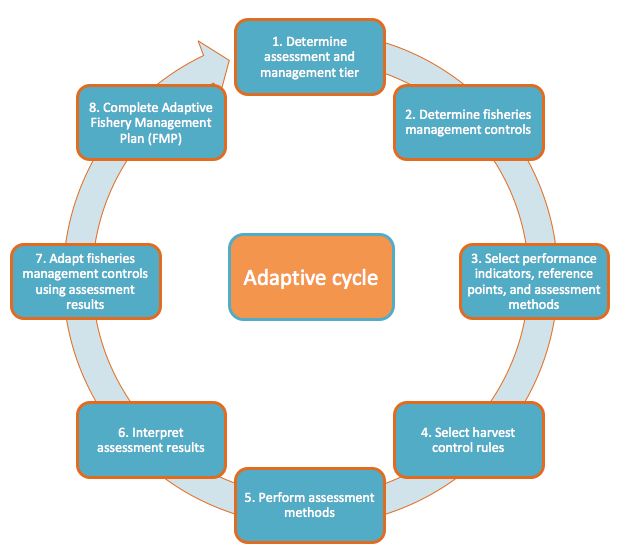
\includegraphics{myMediaFolder/media/2_image1.png}
\caption{\label{fig:schematic}8 steps of the AFAM Toolkit}
\end{figure}

\begin{enumerate}
\def\labelenumi{\arabic{enumi}.}
\item
  \protect\hyperlink{Step1}{Step 1 -- Determine Assessment and
  Management Tier}

  \begin{enumerate}
  \def\labelenumii{\alph{enumii}.}
  \tightlist
  \item
    Your assessment and management tier is based on the data you have
    available and will determine what assessment and management options
    you have at your disposal
  \end{enumerate}
\item
  \protect\hyperlink{Step2}{Step 2 -- Determine Appropriate Fisheries
  Management Controls}

  \begin{enumerate}
  \def\labelenumii{\alph{enumii}.}
  \tightlist
  \item
    Fishery management controls are what allow managers to limit aspects
    of fishing behavior to limit fishing mortality or to protect key
    biological or ecological function (i.e., Total Allowable Catch or
    seasonal closures to protect spawning aggregations)
  \end{enumerate}
\item
  \protect\hyperlink{Step3}{Step 3 -- Select Performance Indicators,
  Reference Points, and Assessment Methods}

  \begin{enumerate}
  \def\labelenumii{\alph{enumii}.}
  \tightlist
  \item
    Performance indicators are numerical values based on data that give
    an indication of how the fishery is performing relative to a
    reference point. Reference points may define either a target where
    you want the fishery to move towards or a limit where you want the
    fishery to stay away from. The assessment method is the technique
    for calculating your performance indicator using available data. For
    example, a performance indicator could be fishing mortality with a
    target reference point of natural mortality. In this case, the
    assessment method to calculate fishing mortality could be Catch
    Curve.
  \end{enumerate}
\item
  \protect\hyperlink{Step4}{Step 4 -- Define Harvest Control Rules}

  \begin{enumerate}
  \def\labelenumii{\alph{enumii}.}
  \tightlist
  \item
    A harvest control rule helps stakeholders to compare performance
    indicators with reference points and adjust fisheries management
    controls accordingly. In other words, a harvest control rule is a
    plan for pre-agreed management actions as a function of variables
    related to the status of stock in question. For example, a simple
    harvest control rule could specify that if fishing mortality is
    above natural mortality, the Total Allowable Catch should be
    reduced.
  \end{enumerate}
\item
  \protect\hyperlink{Step5}{Step 5 - Perform Assessment Methods}

  \begin{enumerate}
  \def\labelenumii{\alph{enumii}.}
  \tightlist
  \item
    You will learn about the various types of assessment methods and use
    the appropriate assessment method to calculate your selected
    performance indicators and reference points. This section provides a
    ``how-to'' guide for using each assessment method. You will use the
    toolkit dashboard to perform the methods.
  \end{enumerate}
\item
  \protect\hyperlink{Step6}{Step 6 -- Interpret Assessment Results}

  \begin{enumerate}
  \def\labelenumii{\alph{enumii}.}
  \tightlist
  \item
    You will interpret your assessment results, together with local
    ecological knowledge and other available data, to determine if a
    management response is required or not.
  \end{enumerate}
\item
  \protect\hyperlink{Step7}{Step 7 -- Adjust Fisheries Management
  Controls Using Defined Harvest Control Rules}

  \begin{enumerate}
  \def\labelenumii{\alph{enumii}.}
  \tightlist
  \item
    You will use the harvest control rules defined in Step 4 and the
    interpretations generated in Step 6 to adjust fisheries management
    controls appropriately.
  \end{enumerate}
\item
  \protect\hyperlink{Step8}{Step 8 -- Complete your Fishery Management
  Plan}

  \begin{enumerate}
  \def\labelenumii{\alph{enumii}.}
  \tightlist
  \item
    You will use the outputs of the AFAM toolkit to fill out a Fishery
    Management Plan template for your fishery. Note that the template
    provided here may need to be adapted to better suit regional
    context.
  \end{enumerate}
\end{enumerate}

\hypertarget{Step1}{\chapter{Step 1 -- Determine Assessment and
Management Tier}\label{Step1}}

\emph{What information do I have, and how can I use it?}

\begin{figure}
\centering
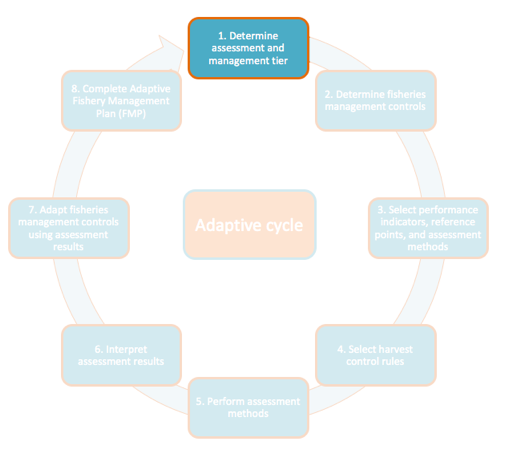
\includegraphics{myMediaFolder/media/Step1.png}
\caption{\label{fig:Step1}Step 1}
\end{figure}

In the first step of this toolkit, you will determine the assessment and
management ``tier'' of your fishery based on the types of information
and data that are available (Figure
\protect\hyperlink{fig:Tiers}{\ref{fig:Tiers}}). Depending on the data
that are available, you will have different options for fisheries
management controls and assessment methods. The tier you determine
during this step will be used throughout the remaining steps of the
toolkit. If your site follows this plan, you will automatically begin
collecting the necessary data to eventually move to Tier 3.

\begin{figure}
\centering
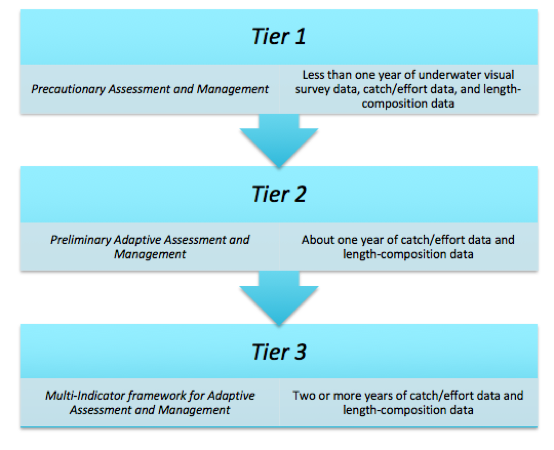
\includegraphics{myMediaFolder/media/Tiers.png}
\caption{\label{fig:Tiers}AFAM Toolkit tier flowchart}
\end{figure}

\section{Step 1a -- Fill out your Data
Inventory}\label{step-1a-fill-out-your-data-inventory}

Fill out your inventory of available data.

\section{Step 1b -- Using your Data Inventory, Determine Assessment and
Management
Tier}\label{step-1b-using-your-data-inventory-determine-assessment-and-management-tier}

Use the following questions to determine which assessment tier is most
appropriate for your site:

\begin{enumerate}
\def\labelenumi{\arabic{enumi}.}
\item
  Do you have two or more years of catch/effort data (from individual
  catch reporting and/or boat intercept or landing site survey)? Do you
  also have two or more years of fishery-dependent length-composition
  survey data?

  \begin{enumerate}
  \def\labelenumii{\alph{enumii}.}
  \item
    \textbf{Yes} -- Use the \emph{Tier 3} category and continue
    collecting data.
  \item
    \textbf{No} - Continue on to question two.
  \end{enumerate}
\item
  Do you have at least one year of catch/effort data (from individual
  catch reporting and/or boat intercept or landing site survey) and
  fishery-dependent length-composition survey data?

  \begin{enumerate}
  \def\labelenumii{\alph{enumii}.}
  \item
    \textbf{Yes -} Use the \emph{Tier 2} category and continue
    collecting data.
  \item
    \textbf{No} --Use the \emph{Tier 1} category.
  \end{enumerate}
\end{enumerate}

The three assessment and management categories are described in more
detail below. We will discuss the specifics of fisheries management
controls and performance indicators in the following steps. As you
collect more and more data over time, your site will be able to move
from one tier to the next.

\emph{Tier 1 -- Precautionary Assessment and Management (for new sites
with less than one year of data)}

Under most scenarios, Tier 1 describes a new site, with no pre-existing
standardized data collection and monitoring program in place. The only
information available will likely come from qualitative information and
local ecological knowledge. Even though little to no data is present,
managers can still perform a basic fisheries assessment and select
precautionary fisheries management controls (FMCs) until more data is
collected. The goal of Tier 1 is to implement precautionary assessment
and management measures that can benefit a fishery of any status until
more data is collected for the fishery. When we are uncertain about the
status and dynamics of a resource, it is prudent to interact with the
resource in a way that minimizes the risks of something `bad' happening.
One of the most effective precautionary management techniques is to
limit the use of destructive fishing gears and/or practices. Another
common precautionary management technique is to protect spawning
aggregations through the implementation of a seasonal closure.

\emph{Tier 2 -- Preliminary Adaptive Assessment and Management (for
sites with one year of data)}

Tier 2 sites will have roughly one year of data that come from some
combination of catch reporting, boat intercept or landing site survey,
or fishery-dependent length-composition surveys. The goal of Tier 2 is
to provide the preliminary assessment and management methods for a
fishery, while continuing to collect more data. A suite of FMCs can also
be used in combination to meet multiple objectives where appropriate.

\emph{Tier 3 -- Multi-Indicator framework for Adaptive Assessment and
Management (for sites with more than one year of data)}

Tier 3 sites will have a time series of data available that can be used
to examine trends in multiple performance indicators and implement FMCs
such based on an improved scientific understanding of stock status.
Under Tier 3, each species should have several performance indicators,
which should ideally come from different data streams, in order to gain
a more complete understanding of the fishery and reduce uncertainty.
Multiple performance indicators from multiple data streams are used to
gain a more complete understanding of the fishery and to reduce the
implications of uncertainty, bias, or error associated with any single
indicator or data stream. Furthermore, corroboration between indicators
can allow for a confident interpretation of fishery performance.
Additionally, with multiple years of data, limits and targets can be
estimated from running averages or the average of the past few years.
Running averages take into account variability in the environment and
the fishery. Ecosystem-level indicators should be included if the
sustainable provision of non-fishery ecosystem services is a management
goal.

\hypertarget{Step2}{\chapter{Step 2 -- Determine Appropriate Fisheries
Management Controls}\label{Step2}}

\emph{What fisheries management controls are appropriate for your
fishery?}

\begin{figure}
\centering
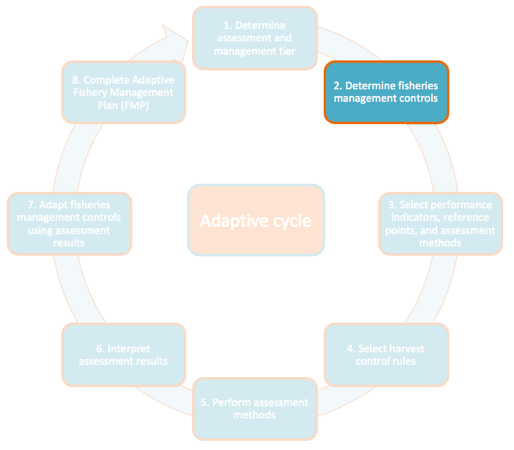
\includegraphics{myMediaFolder/media/Step2.png}
\caption{\label{fig:Step2}Step 2}
\end{figure}

\hypertarget{Step2a}{\section{Step 2a -- Summarize and Qualitatively
Assess Any Existing Fisheries Management Controls}\label{Step2a}}

As an important first step, summarize any existing fisheries management
controls that may affect your site. If there are no existing FMCs, skip
to \protect\hyperlink{Step2b}{Step 2b}.

Qualitatively assess how existing fisheries management controls are
performing. This will help determine whether or not these controls are
appropriate, or if other or additional controls should be used instead.
Think about the following considerations:

\begin{itemize}
\item
  \textbf{Who mandates this FMC?} Is it locally mandated (in which case
  it could potentially be modified or removed), or is it mandated by a
  higher body (such as a regional or national body -- this may make the
  FMC more difficult to modify or remove)? This can help frame a
  discussion around whether or not this FMC could be modified or
  removed.
\item
  \textbf{What is the cost of this FMC?} Does it require expensive data
  collection or enforcement?
\item
  \textbf{What is the level of compliance with this FMC?}
\item
  \textbf{What is public attitude towards this FMC?}
\item
  \textbf{Are current FMCs helping the fishery reach its goals?} You may
  use Table \ref{tab:fmcs-bio}, Table \ref{tab:fmcs-eco}, and Table
  \ref{tab:fmcs-social} to see common goals of many FMCs and determine
  if the goals of your fishery are being met.
\item
  \textbf{What are other implementation pros/cons}?
\end{itemize}

Based on this qualitative assessment, you may be happy with the current
set of FMCs in which case you can skip to
\protect\hyperlink{Step2c}{Step 2c}. Alternatively, if the FMCs are not
performing as your community may wish, proceed to
\protect\hyperlink{Step2b}{Step 2b} to explore selecting different FMCs.
Either way, you will quantitatively assess how well FMCs are doing in
terms of fisheries performance in \protect\hyperlink{Step5}{Step 5} by
performing data-limited assessments using any available data. Based on
this quantitative evaluation, you may wish to change FMCs during the
next iteration of the AFAM cycle.

\hypertarget{Step2b}{\section{Step 2b -- Preliminary Selection of New
Fisheries Management Controls}\label{Step2b}}

Fisheries managers have a number of different fisheries management
controls (FMCs) to choose from to manage their fishery goals. Many FMCs
are designed with the primary objective of limiting fishing mortality
such as catch limits; however, other FMCs are designed to protect
certain biological or ecological functions in an ecosystem such as
seasonal closures to protect spawning aggregations. Descriptions of
commonly used FMCs are listed in Table \ref{tab:fmcs}. This table also
includes data requirements and enforcement considerations for the
implementation of each FMC. Additionally,
\protect\hyperlink{case-studies}{case studies} are presented below for
each FMC that describe situations where the FMC has been implemented in
a small-scale fishery. These case studies present some of the
opportunities, challenges, and implications these different FMCs bring
to small-scale fisheries.

To select a list of preliminary fisheries management controls, use the
six questions in the decision tree below (Figure
\ref{fig:decision-tree}) as a general guide and first step to determine
what FMCs may be appropriate for your fishery. However, conditions
occurring in your specific fishery must be carefully considered as well
as the community goals for management. Additionally, while this figure
is one tool for helping select the type of FMC (i.e., minimum size
limit) it does no provide guidance on the specific FMC that should be
implemented (i.e., what that minimum size limit should be)
\protect\hyperlink{Step2c}{Steps 2c} and \protect\hyperlink{Step2d}{2d}
are designed to guide additional considerations when determining
appropriate and specific FMCs.

\begin{figure}
\centering
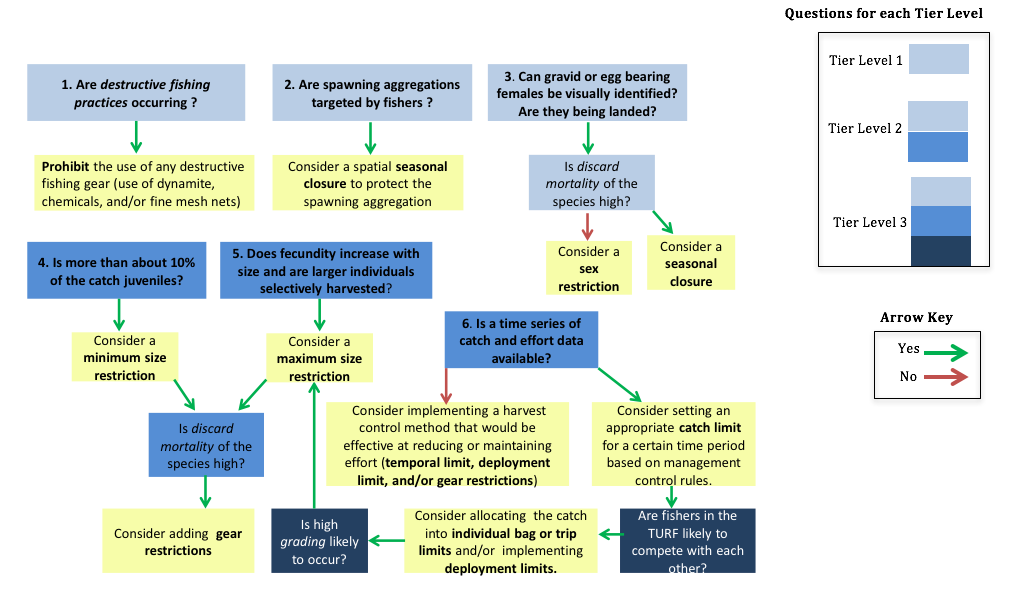
\includegraphics{myMediaFolder/media/FMCs.png}
\caption{\label{fig:decision-tree}Decision tree to help identify potentially
appropriate Fisheries Management Control(s)}
\end{figure}

\hypertarget{Step2c}{\section{Step 2c -- Consider Applying Additional
Fisheries Management Controls to Better Meet Goals}\label{Step2c}}

There is no prescriptive method for determining the `perfect'
combination of FMCs for every site because the most appropriate FMCs
will greatly depend on the specific conditions and characteristics of
the fishery and surrounding community. The following 6 steps, along with
the information in in Table \ref{tab:fmcs-bio}, Table
\ref{tab:fmcs-eco}, and Table \ref{tab:fmcs-social}, can serve as a
guide to help identify a set of FMCs that may be effective at meeting
your site's management goals.

\begin{enumerate}
\def\labelenumi{\arabic{enumi}.}
\item
  Find the FMC(s) that were either existing
  (\protect\hyperlink{Step2a}{Step 2a}) or newly selected
  (\protect\hyperlink{Step2b}{Step 2b}) in Table \ref{tab:fmcs-bio},
  Table \ref{tab:fmcs-eco}, and Table \ref{tab:fmcs-social}. These
  tables describe potential negative or positive impacts of each FMC on
  common biological, ecological, and socioeconomic fishery management
  objectives.
\item
  Identify which of the management objectives in the first row of Table
  \ref{tab:fmcs-bio}, Table \ref{tab:fmcs-eco}, and Table
  \ref{tab:fmcs-social} align with the site's management goals.
\item
  Review the potential impact of each FMC being considered for your site
  on each of your management objectives.
\item
  Determine if the preliminary selection of FMC(s) will conflict with or
  fail to accomplish any of your site's management goals. For example, a
  catch limit may have been identified as an appropriate FMC to control
  harvest at a site but additional management goals of the site may be
  to protect habitat and reduce bycatch. Table \ref{tab:fmcs-eco} shows
  that implementing a catch limit may result in an increase in bycatch
  rates and increased habitat damage if implemented without any other
  FMCs.
\item
  Use Table \ref{tab:fmcs-bio}, Table \ref{tab:fmcs-eco}, and Table
  \ref{tab:fmcs-social} to identify FMC(s) that are associated with
  positive impacts on the sites management objectives. FMC(s) identified
  here can be chosen in combination with FMC(s) identified in
  \protect\hyperlink{Step2a}{Step 2a} to meet multiple management
  objectives. For example, in some fisheries, combining gear
  restrictions with catch limits may be effective at controlling
  harvest, and reducing bycatch and habitat damage.
\item
  In Table \ref{tab:fmcs-bio}, Table \ref{tab:fmcs-eco}, and Table
  \ref{tab:fmcs-social}, some FMCs have similar impacts across
  management objectives and it may be unclear which FMC is most
  appropriate for your site. To determine the most appropriate FMC(s)
  for your site, consider the ``ease of implementation'' for each FMC
  listed in Table \ref{tab:fmcs} and how it aligns with the specific
  conditions and characteristics the site.
\end{enumerate}

\hypertarget{Step2d}{\section{Step 2d -- Consider Implications with
Relevant Stakeholders}\label{Step2d}}

Before finalizing which FMC(s)will be implemented at your site, consider
how fishers (as well as other stakeholders such as middlemen,
enforcement organizations, etc.) may respond to this management control
by considering the following questions:

\begin{itemize}
\item
  What management methods have successfully been implemented in the
  past?
\item
  Can this management method be effectively implemented and enforced?
\item
  Is this method socially and politically feasible, and will fishers
  comply with it?
\end{itemize}

The ability of the selected FMCs to meet the stated community objectives
should be discussed will all relevant stakeholders, along with any
potential tradeoffs of implementing the selected FMC(s).

Additionally, prior to implementing FMC(s), any existing social survey
data should be reviewed. Social survey data can be used to provide
insight into individual attitudes towards fishery management in your
community. Any information on enforcement should also be reviewed to
gain a better understanding of the likelihood of compliance with
implementation of new FMCs.

\section{Step 2e -- General Guidance for Setting Effective FMCs for the
First Time}\label{Step2e}

\textbf{\emph{Note -- This step is only applicable when developing your
Adaptive Fisheries Assessment and Management Framework for the first
time. In following years, you will use harvest control rules (defined
later) to adaptively adjust these initial controls.}}

Once you have finalized your list of FMCs that will be implemented in
your community, you will need to define the specifics of the FMC for the
first time. For example, what will your catch limit actually be? The
specifics will depend on the status of your site's resources, the
population dynamics of the targeted species at the site, and your site's
specific management objectives. If you believe target species are
depleted, if little information is available, and/or if enforcement or
compliance is low, we recommend taking a precautionary approach using
the following suggestions:

\begin{itemize}
\item
  \textbf{Catch Limit} - Set annual catch limit at or below the previous
  year's total catch
\item
  \textbf{Bag or Trip Limit} - Divide the previous year's catch by the
  number of fishers participating in the fishery. Set the Bag or trip
  limit at that level or below
\item
  \textbf{Size limit} - Set a minimum size limit above the minimum size
  at maturity. A maximum size limit may also be set to protect
  \emph{megaspawners}.
\item
  \textbf{Temporal limits} -- Close the fishery during biologically
  sensitive times or during times (or areas) when the catchability of
  species greatly increases (such as Spawning aggregations).
\item
  \textbf{Vessel/gear restrictions} - Gear and vessel restrictions
  should be set that minimize the impact of the fishery on habitat. Gear
  dimensions should also be set that reduce bycatch. For example, small
  mesh size in nets may be prohibited to reduce the landings of
  individuals below reproductive maturity.
\item
  \textbf{Deployment Limits} - Initial deployment limits may be set to
  restrict the number of gears being used to the same number of gears
  that were used in the previous year or below.
\item
  \textbf{Sex specific} - Ban the take of females that are egg-bearing
  or the take of females during a biologically sensitive period.
\item
  \textbf{Protection of Ecologically Important Species} - Restrict
  fishing of specific species in order to protect key ecological
  function, such as herbivorous parrotfish that control macroalgae
  cover.
\end{itemize}

\begin{longtable}[]{@{}lllll@{}}
\caption{\label{tab:fmcs} Descriptions and implementation considerations for
different fisheries management controls}\tabularnewline
\toprule
\begin{minipage}[b]{0.17\columnwidth}\raggedright\strut
\textbf{Fisheries Management Control}\strut
\end{minipage} & \begin{minipage}[b]{0.17\columnwidth}\raggedright\strut
\textbf{Primary Objective}\strut
\end{minipage} & \begin{minipage}[b]{0.17\columnwidth}\raggedright\strut
\textbf{Descripti on}\strut
\end{minipage} & \begin{minipage}[b]{0.17\columnwidth}\raggedright\strut
\textbf{Minimum Data Requirement s}\strut
\end{minipage} & \begin{minipage}[b]{0.17\columnwidth}\raggedright\strut
\textbf{Enforceme nt}\strut
\end{minipage}\tabularnewline
\midrule
\endfirsthead
\toprule
\begin{minipage}[b]{0.17\columnwidth}\raggedright\strut
\textbf{Fisheries Management Control}\strut
\end{minipage} & \begin{minipage}[b]{0.17\columnwidth}\raggedright\strut
\textbf{Primary Objective}\strut
\end{minipage} & \begin{minipage}[b]{0.17\columnwidth}\raggedright\strut
\textbf{Descripti on}\strut
\end{minipage} & \begin{minipage}[b]{0.17\columnwidth}\raggedright\strut
\textbf{Minimum Data Requirement s}\strut
\end{minipage} & \begin{minipage}[b]{0.17\columnwidth}\raggedright\strut
\textbf{Enforceme nt}\strut
\end{minipage}\tabularnewline
\midrule
\endhead
\begin{minipage}[t]{0.19\columnwidth}\raggedright\strut
Catch Limit\strut
\end{minipage} & \begin{minipage}[t]{0.19\columnwidth}\raggedright\strut
Limit fishing mortality\strut
\end{minipage} & \begin{minipage}[t]{0.19\columnwidth}\raggedright\strut
Sets an upper limit on how many fish can be removed by a fishery in a
given time. This can be for an entire fishery or can be allocated to
individuals or groups of individuals (such as a fisher association ).
Limits can be set for individual species or groups of species (also
known as a ``quota basket). If set correctly and fishers' incentives are
aligned, catch limits are the most direct way of managing fishing
mortality. Catch limits can be set on the species basis but also
aggregate level based on similar life history traits and vulnerabili ty.
If the incentives are not aligned and rights are not allocated, catch
limits can perpetuate the race to fish that may lead to safety issues
and destructive fishing practices (gear lost, highgrading , etc.)

Need at least one year's worth of catch and effort data to know where to
set the limit.\strut
\end{minipage} & \begin{minipage}[t]{0.19\columnwidth}\raggedright\strut
A time series of catch and effort data; information on the stock's
productivit y (length-bas ed DLSA methods can be used for proxies); life
history information\strut
\end{minipage} & \begin{minipage}[t]{0.19\columnwidth}\raggedright\strut
Catch limits (individual or group allocated) can be enforced if landings
are relatively centralized but may be more difficult if landing sites
are more dispersed. Any catch limit program will have associated
monitoring costs for implementat ion to be effective.\strut
\end{minipage}\tabularnewline
\begin{minipage}[t]{0.17\columnwidth}\raggedright\strut
Bag or Trip Limit\strut
\end{minipage} & \begin{minipage}[t]{0.17\columnwidth}\raggedright\strut
Limit fishing mortality\strut
\end{minipage} & \begin{minipage}[t]{0.17\columnwidth}\raggedright\strut
Limits the number or weight of fish that can be landed by an individual
fisher or vessel on a single day or fishing trip. If no illegal
discarding is occurring, than bag limits and trip limits based on number
of fish allowed to catch can directly control fishing mortality. Can
perpetuate high grading and illegal discarding.\strut
\end{minipage} & \begin{minipage}[t]{0.17\columnwidth}\raggedright\strut
Time series of catch and effort data, information on the stock's
productivit y (length-bas ed DLSA methods can be used for proxies), and
total number of fishermen participati ng in a fishery\strut
\end{minipage} & \begin{minipage}[t]{0.17\columnwidth}\raggedright\strut
Can be enforced if landings are relatively centralized but may be more
difficult if landing sites are more dispersed. Monitoring for every
vessel or individual in a fishery will result in significant implementat
ion costs.\strut
\end{minipage}\tabularnewline
\begin{minipage}[t]{0.17\columnwidth}\raggedright\strut
Size Limit\strut
\end{minipage} & \begin{minipage}[t]{0.17\columnwidth}\raggedright\strut
Limit fishing mortality\strut
\end{minipage} & \begin{minipage}[t]{0.17\columnwidth}\raggedright\strut
Sets minimum and/or maximum bounds on the size of fish that can be
legally landed in a fishery. Size limits can protect age-structu re by
controlling the size selectivity of the fishery to ensure fish have the
opportunity to spawn before being caught. However, the biology of the
species must be considered carefully because size limits can result in
unintended, negative consequence s. Size limits don't directly control
fishing mortality and may cause size truncation over time by removing
the largest individuals from a fishery\strut
\end{minipage} & \begin{minipage}[t]{0.17\columnwidth}\raggedright\strut
Size at maturity and/or size of megaspawner s; discard mortality rates
for targeted species are helpful\strut
\end{minipage} & \begin{minipage}[t]{0.17\columnwidth}\raggedright\strut
Can be enforced if landings are relatively centralized but may be more
difficult if landing sites are more dispersed. Monitoring is straightfor
ward and does not have many associated implementat ion costs.\strut
\end{minipage}\tabularnewline
\begin{minipage}[t]{0.17\columnwidth}\raggedright\strut
Temporal Limit\strut
\end{minipage} & \begin{minipage}[t]{0.17\columnwidth}\raggedright\strut
Limit fishing mortality\strut
\end{minipage} & \begin{minipage}[t]{0.17\columnwidth}\raggedright\strut
Restricts the time period over which a fish can be legally landed. If
fishing mortality doesn't increase before or after the closure,
temporary closures allow marine resources to increase without
disturbance to ensure fish grow bigger and new recruits enter the
fishery. Perpetuates the race to fish before and after the closure.
Increases fishing effort before and after the closure. Doesn't directly
manage fishing mortality.\strut
\end{minipage} & \begin{minipage}[t]{0.17\columnwidth}\raggedright\strut
Temporal dynamics of fishing effort; temporal characteris tics or
behavior of target species; information on the relationshi p between
catch and effort is helpful\strut
\end{minipage} & \begin{minipage}[t]{0.17\columnwidth}\raggedright\strut
Can be enforced if landings are relatively centralized but may be more
difficult if landing sites are more dispersed. Temporal limits are more
straightfor ward to monitor if the limit covers all species, but may be
more difficult if the limit only covers a certain species in the
fishery.\strut
\end{minipage}\tabularnewline
\begin{minipage}[t]{0.17\columnwidth}\raggedright\strut
Gear Restriction s -- Gear Type\strut
\end{minipage} & \begin{minipage}[t]{0.17\columnwidth}\raggedright\strut
Limit fishing mortality\strut
\end{minipage} & \begin{minipage}[t]{0.17\columnwidth}\raggedright\strut
Restricts the type of fishing gear allowed to participate in a fishery
(including banning destructive fishing gear such as dynamite, cyanide,
and fine mesh nets) but doesn't directly manage fishing mortality.\strut
\end{minipage} & \begin{minipage}[t]{0.17\columnwidth}\raggedright\strut
Information on the relationshi p between gear characteris tics, fishing
effort, and selectivity . If only banning destructive fishing gear, no
data is required.\strut
\end{minipage} & \begin{minipage}[t]{0.17\columnwidth}\raggedright\strut
Gear restriction s are relatively straightfor ward to enforce however,
gathering information required for an effective implementat ion can be
costly\emph{.} If only banning destructive fishing gear, there are low
upfront costs but ongoing monitoring costs should be considered.\strut
\end{minipage}\tabularnewline
\begin{minipage}[t]{0.17\columnwidth}\raggedright\strut
Gear Restriction s -- Gear Number (also known as Deployment
Limits)\strut
\end{minipage} & \begin{minipage}[t]{0.17\columnwidth}\raggedright\strut
Limit fishing mortality\strut
\end{minipage} & \begin{minipage}[t]{0.17\columnwidth}\raggedright\strut
Places a cap on the number of gears each fisher can use (such as the
number of fixed traps or the number of hooks on a line). Does not
directly manage fishing mortality. Can reduce the number of gear in the
water thus decreasing habitat impacts..\strut
\end{minipage} & \begin{minipage}[t]{0.17\columnwidth}\raggedright\strut
Current fishing effort levels in terms of number of gears; information
on the relationshi p between catch and effort is helpful\strut
\end{minipage} & \begin{minipage}[t]{0.17\columnwidth}\raggedright\strut
The ease and cost of enforcement will depend on how easily fishing gears
can be observed.\strut
\end{minipage}\tabularnewline
\begin{minipage}[t]{0.17\columnwidth}\raggedright\strut
Sex-Specifi c Controls\strut
\end{minipage} & \begin{minipage}[t]{0.17\columnwidth}\raggedright\strut
Limit fishing mortality\strut
\end{minipage} & \begin{minipage}[t]{0.17\columnwidth}\raggedright\strut
Protect reproductiv ely important individuals by setting sex-specifi c
prohibition s on fishing activity.\strut
\end{minipage} & \begin{minipage}[t]{0.17\columnwidth}\raggedright\strut
Information on reproductiv e traits and sex ratios\strut
\end{minipage} & \begin{minipage}[t]{0.17\columnwidth}\raggedright\strut
Sex-specifi c controls are straightfor ward to enforce if there are
obvious differences between the sexes. Monitoring costs will depend on
how easily the catch can be observed.\strut
\end{minipage}\tabularnewline
\begin{minipage}[t]{0.17\columnwidth}\raggedright\strut
Seasonal Closures to Protect Vulnerable Life History Stages\strut
\end{minipage} & \begin{minipage}[t]{0.17\columnwidth}\raggedright\strut
Protect vulnerable life history stages\strut
\end{minipage} & \begin{minipage}[t]{0.17\columnwidth}\raggedright\strut
Protect vulnerable life history stages by restricting the fishery during
certain seasons. Seasonal spawning closures allow spawning to occur
without disruption to ensure recruits enter the fishery. Perpetuates the
race to fish before and after closure. Increases fishing effort before
and after the closure. Doesn't directly manage fishing mortality.\strut
\end{minipage} & \begin{minipage}[t]{0.17\columnwidth}\raggedright\strut
Information on seasonal behavior such as spawning aggregation s and
migrations, and the temporal and spatial variability of these
behaviors\strut
\end{minipage} & \begin{minipage}[t]{0.17\columnwidth}\raggedright\strut
Can be enforced if landings are relatively centralized but may be more
difficult if landing sites are more dispersed. Seasonal closures are
more straightfor ward to monitor if the closure covers all species, but
may be more difficult if the closure only covers a certain species in
the fishery.\strut
\end{minipage}\tabularnewline
\begin{minipage}[t]{0.17\columnwidth}\raggedright\strut
Protection of Ecologicall y Important Species\strut
\end{minipage} & \begin{minipage}[t]{0.17\columnwidth}\raggedright\strut
Protect ecological function\strut
\end{minipage} & \begin{minipage}[t]{0.17\columnwidth}\raggedright\strut
Restrict fishing of specific species in order to protect key ecological
functions. Does not directly control fishing mortality.\strut
\end{minipage} & \begin{minipage}[t]{0.17\columnwidth}\raggedright\strut
Information on ecological interaction s and roles\strut
\end{minipage} & \begin{minipage}[t]{0.17\columnwidth}\raggedright\strut
Protection of ecologicall y important species can be straightfor ward
but monitoring costs will depend on how easily the species and fishery
catch can be observed.\strut
\end{minipage}\tabularnewline
\bottomrule
\end{longtable}

\begin{longtable}[]{@{}llll@{}}
\caption{\label{tab:fmcs-bio} Effectiveness of different fisheries
management controls in meeting biological objectives}\tabularnewline
\toprule
\begin{minipage}[b]{0.22\columnwidth}\raggedright\strut
\textbf{Fisheries Management Control}\strut
\end{minipage} & \begin{minipage}[b]{0.22\columnwidth}\raggedright\strut
\textbf{Protect Spawning Stock Biomass (SSB)}\strut
\end{minipage} & \begin{minipage}[b]{0.22\columnwidth}\raggedright\strut
\textbf{Protect Age-Structure}\strut
\end{minipage} & \begin{minipage}[b]{0.22\columnwidth}\raggedright\strut
\textbf{Protect Vulnerable Life History Stages}\strut
\end{minipage}\tabularnewline
\midrule
\endfirsthead
\toprule
\begin{minipage}[b]{0.22\columnwidth}\raggedright\strut
\textbf{Fisheries Management Control}\strut
\end{minipage} & \begin{minipage}[b]{0.22\columnwidth}\raggedright\strut
\textbf{Protect Spawning Stock Biomass (SSB)}\strut
\end{minipage} & \begin{minipage}[b]{0.22\columnwidth}\raggedright\strut
\textbf{Protect Age-Structure}\strut
\end{minipage} & \begin{minipage}[b]{0.22\columnwidth}\raggedright\strut
\textbf{Protect Vulnerable Life History Stages}\strut
\end{minipage}\tabularnewline
\midrule
\endhead
\begin{minipage}[t]{0.22\columnwidth}\raggedright\strut
Catch Limit\strut
\end{minipage} & \begin{minipage}[t]{0.22\columnwidth}\raggedright\strut
Catch limits directly protect SSB\strut
\end{minipage} & \begin{minipage}[t]{0.22\columnwidth}\raggedright\strut
Catch limits do not directly protect age-structure and may have a
negative impact on the age-structure because fishers are choosing an
overall quantity indiscriminate of size or age.\strut
\end{minipage} & \begin{minipage}[t]{0.22\columnwidth}\raggedright\strut
Catch limits do not directly protect vulnerable life history
stages\strut
\end{minipage}\tabularnewline
\begin{minipage}[t]{0.22\columnwidth}\raggedright\strut
Bag or Trip Limit\strut
\end{minipage} & \begin{minipage}[t]{0.22\columnwidth}\raggedright\strut
Bag or trip limits do not directly protect SSB because a increase in
total fishing effort can still occur\strut
\end{minipage} & \begin{minipage}[t]{0.22\columnwidth}\raggedright\strut
Bag or trip limits do not directly protect age-structure and may
incentivize fishers to choose larger and more valuable fish than they
would otherwise catch, which may have a negative impact on age
structure\strut
\end{minipage} & \begin{minipage}[t]{0.22\columnwidth}\raggedright\strut
Bag or trip limits do not directly protect vulnerable life history
stages\strut
\end{minipage}\tabularnewline
\begin{minipage}[t]{0.22\columnwidth}\raggedright\strut
Size Limit\strut
\end{minipage} & \begin{minipage}[t]{0.22\columnwidth}\raggedright\strut
Size limits do not directly protect SSB because they do not control
total harvest of a stock\strut
\end{minipage} & \begin{minipage}[t]{0.22\columnwidth}\raggedright\strut
Size limits can protect age-structure by controlling the size
selectivity of the fishery if discard mortality rates are low. However,
the biology of the species must be considered carefully because size
limits can result in unintended, negative consequences such as size
structure truncation.\strut
\end{minipage} & \begin{minipage}[t]{0.22\columnwidth}\raggedright\strut
Size limits may protect vulnerable life history stages if those stages
are associated with a certain size.\strut
\end{minipage}\tabularnewline
\begin{minipage}[t]{0.22\columnwidth}\raggedright\strut
Temporal Limit\strut
\end{minipage} & \begin{minipage}[t]{0.22\columnwidth}\raggedright\strut
Temporal limits do not directly protect SSB because they do not control
total harvest of a stock\strut
\end{minipage} & \begin{minipage}[t]{0.22\columnwidth}\raggedright\strut
Temporal limits do not protect age-structure and may have a negative
impact on the age-structure because fishers may race to catch as much
fish as they can, while they can, indiscriminate of size or age.\strut
\end{minipage} & \begin{minipage}[t]{0.22\columnwidth}\raggedright\strut
Temporal limits can be designed to protect vulnerable life history
stages associated with the timeframe of the limit.\strut
\end{minipage}\tabularnewline
\begin{minipage}[t]{0.22\columnwidth}\raggedright\strut
Gear Restrictions -- Gear Type\strut
\end{minipage} & \begin{minipage}[t]{0.22\columnwidth}\raggedright\strut
Gear type restrictions do not directly protect SSB because they do not
control total harvest of a stock\strut
\end{minipage} & \begin{minipage}[t]{0.22\columnwidth}\raggedright\strut
Gear type restrictions can be implemented to protect age-structure by
modifying selectivity to allow individuals of a specific size to escape
harvest.\strut
\end{minipage} & \begin{minipage}[t]{0.22\columnwidth}\raggedright\strut
Gear type restrictions may protect vulnerable life history stages\strut
\end{minipage}\tabularnewline
\begin{minipage}[t]{0.22\columnwidth}\raggedright\strut
Gear Restrictions -- Gear Number (also known as Deployment Limits)\strut
\end{minipage} & \begin{minipage}[t]{0.22\columnwidth}\raggedright\strut
Gear number restrictions do not directly protect SSB because an increase
in effort may occur if new fishers join the fishery\strut
\end{minipage} & \begin{minipage}[t]{0.22\columnwidth}\raggedright\strut
Gear number restrictions do not directly protect age structure\strut
\end{minipage} & \begin{minipage}[t]{0.22\columnwidth}\raggedright\strut
Gear number restrictions do not directly protect vulnerable life history
stages\strut
\end{minipage}\tabularnewline
\begin{minipage}[t]{0.22\columnwidth}\raggedright\strut
Sex-Specific Controls\strut
\end{minipage} & \begin{minipage}[t]{0.22\columnwidth}\raggedright\strut
Sex-specific controls protect the spawning biomass of the sex targeted
by the regulation\strut
\end{minipage} & \begin{minipage}[t]{0.22\columnwidth}\raggedright\strut
Sex-specific controls do not protect age-structure and may have negative
consequences for age-structure because fishers may target the largest
individuals of the sex that is not protected\strut
\end{minipage} & \begin{minipage}[t]{0.22\columnwidth}\raggedright\strut
Sex-specific controls may protect a vulnerable life stage if that occurs
for a specific sex\strut
\end{minipage}\tabularnewline
\begin{minipage}[t]{0.22\columnwidth}\raggedright\strut
Seasonal Closures to Protect Vulnerable Life History Stages\strut
\end{minipage} & \begin{minipage}[t]{0.22\columnwidth}\raggedright\strut
Seasonal closures protect spawning biomass during specific seasons\strut
\end{minipage} & \begin{minipage}[t]{0.22\columnwidth}\raggedright\strut
Seasonal closures do not directly protect age-structure\strut
\end{minipage} & \begin{minipage}[t]{0.22\columnwidth}\raggedright\strut
Seasonal closures protect seasonal vulnerable life history stages\strut
\end{minipage}\tabularnewline
\begin{minipage}[t]{0.22\columnwidth}\raggedright\strut
Protection of Ecologically Important Species\strut
\end{minipage} & \begin{minipage}[t]{0.22\columnwidth}\raggedright\strut
Protection of ecologically important species protects the SSB of the
species of interest but does not directly protect SSB of other target
species\strut
\end{minipage} & \begin{minipage}[t]{0.22\columnwidth}\raggedright\strut
Protection of ecologically important species protects the age-structure
of the protected population but does not directly protect age-structure
of other target species\strut
\end{minipage} & \begin{minipage}[t]{0.22\columnwidth}\raggedright\strut
Protection of ecologically important species does not directly protect
vulnerable life history stages\strut
\end{minipage}\tabularnewline
\bottomrule
\end{longtable}

\begin{longtable}[]{@{}lll@{}}
\caption{\label{tab:fmcs-eco} Effectiveness of different fisheries
management controls in meeting ecological objectives}\tabularnewline
\toprule
\begin{minipage}[b]{0.30\columnwidth}\raggedright\strut
\textbf{Fisheries Management Control}\strut
\end{minipage} & \begin{minipage}[b]{0.30\columnwidth}\raggedright\strut
\textbf{Protect Habitat}\strut
\end{minipage} & \begin{minipage}[b]{0.30\columnwidth}\raggedright\strut
\textbf{Reduce Bycatch and/or Discards}\strut
\end{minipage}\tabularnewline
\midrule
\endfirsthead
\toprule
\begin{minipage}[b]{0.30\columnwidth}\raggedright\strut
\textbf{Fisheries Management Control}\strut
\end{minipage} & \begin{minipage}[b]{0.30\columnwidth}\raggedright\strut
\textbf{Protect Habitat}\strut
\end{minipage} & \begin{minipage}[b]{0.30\columnwidth}\raggedright\strut
\textbf{Reduce Bycatch and/or Discards}\strut
\end{minipage}\tabularnewline
\midrule
\endhead
\begin{minipage}[t]{0.30\columnwidth}\raggedright\strut
Catch Limit\strut
\end{minipage} & \begin{minipage}[t]{0.30\columnwidth}\raggedright\strut
Catch limits do not protect habitat and may have a negative impact on
habitat unless the use of excessive gear that could damage habitat is
mitigated by an individual allocation that stops the race to fish.\strut
\end{minipage} & \begin{minipage}[t]{0.30\columnwidth}\raggedright\strut
Bycatch can often increase under a catch limit if there is not a limit
for bycatch species along with target species and/or if a single-species
catch limit has been reached in a multi-species fishery.\strut
\end{minipage}\tabularnewline
\begin{minipage}[t]{0.30\columnwidth}\raggedright\strut
Bag or Trip Limit\strut
\end{minipage} & \begin{minipage}[t]{0.30\columnwidth}\raggedright\strut
Bag or trip limits do not directly protect habitat\strut
\end{minipage} & \begin{minipage}[t]{0.30\columnwidth}\raggedright\strut
Bag or trip limits often result in an increase in bycatch and/or
discards because of the incentives to catch the largest and highest
value fish, and/or if a single-species catch limit has been reached in a
multi-species fishery\strut
\end{minipage}\tabularnewline
\begin{minipage}[t]{0.30\columnwidth}\raggedright\strut
Size Limit\strut
\end{minipage} & \begin{minipage}[t]{0.30\columnwidth}\raggedright\strut
Size limits do not directly protect habitat\strut
\end{minipage} & \begin{minipage}[t]{0.30\columnwidth}\raggedright\strut
Bycatch and/or discards can increase under a size limit because under-
or over-sized individuals must be discarded. High discard mortality
rates can result in size-limits having unintended, negative
consequences. Discard mortality may be less of a problem for
invertebrates, however.\strut
\end{minipage}\tabularnewline
\begin{minipage}[t]{0.30\columnwidth}\raggedright\strut
Temporal Limit\strut
\end{minipage} & \begin{minipage}[t]{0.30\columnwidth}\raggedright\strut
Temporal limits do not protect habitat and may have a negative impact if
excessive gear is set during the race-to-fish and is lost or
abandoned\strut
\end{minipage} & \begin{minipage}[t]{0.30\columnwidth}\raggedright\strut
Temporal limits can be designed to reduce bycatch if a fishery
interaction with a bycatch species is seasonal. Temporal limits not
designed to reduce bycatch may cause an increase in bycatch because
fishers are less selective during the race-to-fish\strut
\end{minipage}\tabularnewline
\begin{minipage}[t]{0.30\columnwidth}\raggedright\strut
Gear Restrictions -- Gear Type\strut
\end{minipage} & \begin{minipage}[t]{0.30\columnwidth}\raggedright\strut
Gear type restrictions do not directly protect habitat but can be
designed to reduce the impact a fishery has on habitat\strut
\end{minipage} & \begin{minipage}[t]{0.30\columnwidth}\raggedright\strut
Gear type restrictions may reduce bycatch by improving selectivity in a
fishery\strut
\end{minipage}\tabularnewline
\begin{minipage}[t]{0.30\columnwidth}\raggedright\strut
Gear Restrictions -- Gear Number (also known as Deployment Limits)\strut
\end{minipage} & \begin{minipage}[t]{0.30\columnwidth}\raggedright\strut
Gear number do not directly protect habitat\strut
\end{minipage} & \begin{minipage}[t]{0.30\columnwidth}\raggedright\strut
Gear number restrictions do not directly reduce bycatch\strut
\end{minipage}\tabularnewline
\begin{minipage}[t]{0.30\columnwidth}\raggedright\strut
Sex-Specific Controls\strut
\end{minipage} & \begin{minipage}[t]{0.30\columnwidth}\raggedright\strut
Sex-specific controls do not directly protect habitat\strut
\end{minipage} & \begin{minipage}[t]{0.30\columnwidth}\raggedright\strut
Sex-specific controls can increase discards because individuals of the
protected sex must be returned to sea and depending on the species may
not survive\strut
\end{minipage}\tabularnewline
\begin{minipage}[t]{0.30\columnwidth}\raggedright\strut
Seasonal Closures to Protect Vulnerable Life History Stages\strut
\end{minipage} & \begin{minipage}[t]{0.30\columnwidth}\raggedright\strut
Seasonal closures do not directly protect habitat and may have a
negative impact on habitat if excessive gear is set during the
race-to-fish and is lost or abandoned\strut
\end{minipage} & \begin{minipage}[t]{0.30\columnwidth}\raggedright\strut
Seasonal closures do not reduce bycatch and can increase bycatch and
discards during the race to fish\strut
\end{minipage}\tabularnewline
\begin{minipage}[t]{0.30\columnwidth}\raggedright\strut
Protection of Ecologically Important Species\strut
\end{minipage} & \begin{minipage}[t]{0.30\columnwidth}\raggedright\strut
Protection of ecologically important species may protect the habitat if
the species of interest plays an important role in maintaining ecosystem
health\strut
\end{minipage} & \begin{minipage}[t]{0.30\columnwidth}\raggedright\strut
Protection of ecologically important species can increase discards
because individuals of the protected species can be discarded to avoid
enforcement penalties.\strut
\end{minipage}\tabularnewline
\bottomrule
\end{longtable}

\begin{longtable}[]{@{}lllll@{}}
\caption{\label{tab:fmcs-social} Effectiveness of different fisheries
management controls in meeting socioeconomic objectives}\tabularnewline
\toprule
\begin{minipage}[b]{0.17\columnwidth}\raggedright\strut
\textbf{Fisheries Management Control}\strut
\end{minipage} & \begin{minipage}[b]{0.17\columnwidth}\raggedright\strut
\textbf{Increase Fisher Profits}\strut
\end{minipage} & \begin{minipage}[b]{0.17\columnwidth}\raggedright\strut
\textbf{Increase Product Quality}\strut
\end{minipage} & \begin{minipage}[b]{0.17\columnwidth}\raggedright\strut
**Maintain Fishing Efficiency\emph{ }\strut
\end{minipage} & \begin{minipage}[b]{0.17\columnwidth}\raggedright\strut
\textbf{Fisher Safety}\strut
\end{minipage}\tabularnewline
\midrule
\endfirsthead
\toprule
\begin{minipage}[b]{0.17\columnwidth}\raggedright\strut
\textbf{Fisheries Management Control}\strut
\end{minipage} & \begin{minipage}[b]{0.17\columnwidth}\raggedright\strut
\textbf{Increase Fisher Profits}\strut
\end{minipage} & \begin{minipage}[b]{0.17\columnwidth}\raggedright\strut
\textbf{Increase Product Quality}\strut
\end{minipage} & \begin{minipage}[b]{0.17\columnwidth}\raggedright\strut
**Maintain Fishing Efficiency\emph{ }\strut
\end{minipage} & \begin{minipage}[b]{0.17\columnwidth}\raggedright\strut
\textbf{Fisher Safety}\strut
\end{minipage}\tabularnewline
\midrule
\endhead
\begin{minipage}[t]{0.17\columnwidth}\raggedright\strut
Catch Limit\strut
\end{minipage} & \begin{minipage}[t]{0.17\columnwidth}\raggedright\strut
Catch limits that are not allocated at an individual level often cause a
\textbf{short-ter m} decrease in fisher profits because the race-to-fis
h incentivize s capital stuffing and may cause market flooding. Once a
depleted stock recovers, there may be a \textbf{long-term } increase in
fisher profits. Effects from the race-to-fis h and capital stuffing may
be reduced in the case of individuall y allocated limits.\strut
\end{minipage} & \begin{minipage}[t]{0.17\columnwidth}\raggedright\strut
If market flooding occurs, product may be frozen or spoil, decreasing
the product value. Eliminating market flooding by eliminating the
race-to-fis h through individual allocation of catch limits can increase
product quality.\strut
\end{minipage} & \begin{minipage}[t]{0.17\columnwidth}\raggedright\strut
Catch limits do not directly impact \textbf{short-ter m} fishing
efficiency. Individual allocation of catch limits can increase fishing
efficiency as the race-to-fis h is stopped and fishers have more control
over when to fish. Once a depleted stock recovers, there may be a
\textbf{long-term } increase in fishing efficiency.\strut
\end{minipage} & \begin{minipage}[t]{0.17\columnwidth}\raggedright\strut
Catch limits may have a negative impact on the safety of fishing because
during the race-to-fis h, fishers may continue fishing even if fishing
conditions become unsafe. Individual allocation of catch limits can have
a positive impact on fisher safety since they can eliminate the
race-to-fis h.\strut
\end{minipage}\tabularnewline
\begin{minipage}[t]{0.17\columnwidth}\raggedright\strut
Bag or Trip Limit\strut
\end{minipage} & \begin{minipage}[t]{0.17\columnwidth}\raggedright\strut
Bag limits often cause a \textbf{short-ter m} decrease in fisher
profits, because fishers are incentivize d to take more trips to
maintain landings, increasing fishing costs. Once a depleted stock
recovers, there may be a \textbf{long-term } increase in fisher
profits.\strut
\end{minipage} & \begin{minipage}[t]{0.17\columnwidth}\raggedright\strut
Product quality may increase under bag or trip limits because there is
an incentive to catch the biggest and highest value/quali ty fish.\strut
\end{minipage} & \begin{minipage}[t]{0.17\columnwidth}\raggedright\strut
Bag or trip limits fishers do not directly impact \textbf{short-ter m}
fishing efficiency. Once a depleted stock recovers, there may be a
\textbf{long-term } increase in fishing efficiency.\strut
\end{minipage} & \begin{minipage}[t]{0.17\columnwidth}\raggedright\strut
Bag or trip limits may have a negative impact on safety if increasing
the number of fishing trips means that they will need to fish in bad
weather\strut
\end{minipage}\tabularnewline
\begin{minipage}[t]{0.17\columnwidth}\raggedright\strut
Size Limit\strut
\end{minipage} & \begin{minipage}[t]{0.17\columnwidth}\raggedright\strut
Size limits do not increase \textbf{short-ter m} fisher profits and may
cause a decrease in landings revenue if a large portion of landings is
over or undersized and needs to be discarded. Once a depleted stock
recovers, there may be a \textbf{long-term } increase in fisher
profits.\strut
\end{minipage} & \begin{minipage}[t]{0.17\columnwidth}\raggedright\strut
Size limits can be implemented to increase product quality if the
quality of the product is related to its size\strut
\end{minipage} & \begin{minipage}[t]{0.17\columnwidth}\raggedright\strut
Size limits do not directly impact \textbf{short-ter m} fishing
efficiency. Once a depleted stock recovers, there may be a
\textbf{long-term } increase in fishing efficiency.\strut
\end{minipage} & \begin{minipage}[t]{0.17\columnwidth}\raggedright\strut
Size limits do not have a direct impact on the fisher safety\strut
\end{minipage}\tabularnewline
\begin{minipage}[t]{0.17\columnwidth}\raggedright\strut
Temporal Limit\strut
\end{minipage} & \begin{minipage}[t]{0.17\columnwidth}\raggedright\strut
Fishers often begin targeting other, less valuable species when a
fishery is closed due to a temporal limit, causing \textbf{short-ter m}
fisher profits to decrease. Once a depleted stock recovers, there may be
a \textbf{long-term } increase in fisher profits.\strut
\end{minipage} & \begin{minipage}[t]{0.17\columnwidth}\raggedright\strut
Fishers often become less selective during the race-to -fish, resulting
in a decrease in product quality\strut
\end{minipage} & \begin{minipage}[t]{0.17\columnwidth}\raggedright\strut
Temporal limits do not directly impact \textbf{short-ter m} fishing
efficiency. Once a depleted stock recovers, there may be a
\textbf{long-term } increase in fishing efficiency.\strut
\end{minipage} & \begin{minipage}[t]{0.17\columnwidth}\raggedright\strut
Temporal limits may have a negative impact on the safety of fishing
because during the race-to-fis h, fishers continue fishing even if
fishing conditions become unsafe\strut
\end{minipage}\tabularnewline
\begin{minipage}[t]{0.17\columnwidth}\raggedright\strut
Gear Restriction s -- Gear Type\strut
\end{minipage} & \begin{minipage}[t]{0.17\columnwidth}\raggedright\strut
Gear type restriction s incentivize fishers to invest and improve in
unregulated dimensions of gear, increasing fishing costs and reducing
\textbf{short-ter m} fisher profits. Once a depleted stock recovers,
there may be a \textbf{long-term } increase in fisher profits.\strut
\end{minipage} & \begin{minipage}[t]{0.17\columnwidth}\raggedright\strut
Gear type restriction s can be designed to increase product quality in a
fishery by improving selectivity of higher value individuals\strut
\end{minipage} & \begin{minipage}[t]{0.17\columnwidth}\raggedright\strut
Gear type restriction s reduce \textbf{short-ter m} fishing efficiency.
Once a depleted stock recovers, there may be a \textbf{long-term }
increase in fishing efficiency.\strut
\end{minipage} & \begin{minipage}[t]{0.17\columnwidth}\raggedright\strut
Gear type restriction s do not typically have a direct impact on fisher
safety (unless banning destructive fishing gear that can have unintended
negative impacts on fisher, such as dynamite).\strut
\end{minipage}\tabularnewline
\begin{minipage}[t]{0.17\columnwidth}\raggedright\strut
Gear Restriction s -- Gear Number (also known as Deployment
Limits)\strut
\end{minipage} & \begin{minipage}[t]{0.17\columnwidth}\raggedright\strut
Gear number restriction s do not directly impact \textbf{short-ter m}
profits but may help stabilize fishing costs. Once a depleted stock
recovers, there may be a \textbf{long-term } increase in fisher
profits.\strut
\end{minipage} & \begin{minipage}[t]{0.17\columnwidth}\raggedright\strut
Gear number restriction s do not have an impact on product quality\strut
\end{minipage} & \begin{minipage}[t]{0.17\columnwidth}\raggedright\strut
Gear number restriction s may reduce \textbf{short-ter m} fishing
efficiency. Once a depleted stock recovers, there may be a
\textbf{long-term } increase in fishing efficiency.\strut
\end{minipage} & \begin{minipage}[t]{0.17\columnwidth}\raggedright\strut
Gear number restriction s do not have a direct impact on fisher
safety\strut
\end{minipage}\tabularnewline
\begin{minipage}[t]{0.17\columnwidth}\raggedright\strut
Sex-Specifi c Controls\strut
\end{minipage} & \begin{minipage}[t]{0.17\columnwidth}\raggedright\strut
Sex-specifi c controls may decrease \textbf{short-ter m} fisher profits
because a portion of the catch must be discarded. Once a depleted stock
recovers, there may be a \textbf{long-term } increase in fisher
profits.\strut
\end{minipage} & \begin{minipage}[t]{0.17\columnwidth}\raggedright\strut
Sex-specifi c controls do not affect product quality unless quality is
related to sex\strut
\end{minipage} & \begin{minipage}[t]{0.17\columnwidth}\raggedright\strut
Sex-specifi c controls do not directly impact \textbf{short-ter m}
fishing efficiency. . Once a depleted stock recovers, there may be a
\textbf{long-term } increase in fishing efficiency.\strut
\end{minipage} & \begin{minipage}[t]{0.17\columnwidth}\raggedright\strut
Sex-specifi c controls do not have a direct impact on fisher
safety\strut
\end{minipage}\tabularnewline
\begin{minipage}[t]{0.17\columnwidth}\raggedright\strut
Seasonal Closures to Protect Vulnerable Life History Stages\strut
\end{minipage} & \begin{minipage}[t]{0.17\columnwidth}\raggedright\strut
Seasonal closures do not increase \textbf{short-ter m} fisher profits
and may cause a decrease in income because fishers often shift to less
valuable species. Once a depleted stock recovers, there may be a
\textbf{long-term } increase in fisher profits.\strut
\end{minipage} & \begin{minipage}[t]{0.17\columnwidth}\raggedright\strut
Seasonal closures can lead to a decrease in product quality as fishers
shift to less desirable species\strut
\end{minipage} & \begin{minipage}[t]{0.17\columnwidth}\raggedright\strut
Seasonal closures do not directly impact \textbf{short-ter m} fishing
efficiency. . Once a depleted stock recovers, there may be an additional
\textbf{long-term } increase in fishing efficiency.\strut
\end{minipage} & \begin{minipage}[t]{0.17\columnwidth}\raggedright\strut
Seasonal closure may have a negative impact on fisher safety because
during the race-to-fis h, fishers may fish in unsafe conditions\strut
\end{minipage}\tabularnewline
\begin{minipage}[t]{0.17\columnwidth}\raggedright\strut
Protection of Ecologicall y Important Species\strut
\end{minipage} & \begin{minipage}[t]{0.17\columnwidth}\raggedright\strut
Protection of ecologicall y important species will decrease
\textbf{short-ter m} fisher profits. Once ecological function improves
and other depleted target stocks recover, there may be a
\textbf{long-term } increase in fisher profits.\strut
\end{minipage} & \begin{minipage}[t]{0.17\columnwidth}\raggedright\strut
Protection of ecologicall y important species may increase the product
quality of other target species if the protected species is prey for the
target species\strut
\end{minipage} & \begin{minipage}[t]{0.17\columnwidth}\raggedright\strut
Protection of ecologicall y important species does not directly impact
\textbf{short-ter m} fishing efficiency. Once a depleted stock recovers,
there may be an additional \textbf{long-term } increase in fishing
efficiency.\strut
\end{minipage} & \begin{minipage}[t]{0.17\columnwidth}\raggedright\strut
Protection of ecologicall y important species does not have an impact on
fisher safety\strut
\end{minipage}\tabularnewline
\bottomrule
\end{longtable}

\hypertarget{case-studies}{\section{Fisheries Management Control Case
Studies}\label{case-studies}}

\textbf{Catch Limits}

In the sea cucumber fishery in the Northern District of New Caledonia,
fishermen noticed a decline in commercial sized sea cucumber known as
sandfish (\emph{Holothuria scabra}) in the early 2000s. After closing
the fishery for a short period of time, they worked with the Fisheries
Department in 2008 to set a total allowable catch (TAC) for the fishery,
which they then allocated into quotas for individual fishermen. The TAC
was set according to the total biomass of legally-sized adult sandfish,
taking into account both abundance and body size. This harvestable
biomass was calculated through sampling of the sandfish population and
was re-assessed periodically. After implementing the TAC, there was an
increase in total sandfish biomass and a 142\% increase in the number of
individuals. There was also an increase in the mean weight of sandfish
and the density of individuals. Due to the increases in the sandfish
population, the fishermen were able to raise the TAC in subsequent
years. They also combined the use of the TAC with a cycle of open and
closed periods of fishing.

\emph{Leopold, M., Cornuet, N., Andrefouet, S., Moenteapo, Z.,
Duvauchelle, C., Raubani, J., Ham, J., \& Dumas, P. (2013). Comanaging
small-scale sea cucumber fisheries in New Caledonia and Vanuatu using
stock biomass estimates to set spatial catch quotas. Environmental
Conservation 40(4), 367-379.}

\textbf{Bag/Trip Limits}

In the recreational gag \emph{(Mycteroperca microlepis}) fishery in the
Gulf of Mexico, bag limits are used to prevent recruitment overfishing.
However, discard mortality rates reduce the efficiency of the fishery.

\emph{Tetzlaff, J.C., Pine, W.E., Allen, M.S., \& Ahrens, R.N.M. (2013).
Effectiveness of size limits and bag limits for managing recreational
fisheries: a case study of the Gulf of Mexico recreational gag fishery.
Bulletin of Marine Science 89(2), 483-502.}

\textbf{Size Limits}

1. In Puerto Rico's spiny lobster (\emph{Panulirus argus}) fishery,
landings, catch per unit effort, and average body size all increased
from 1988-2001, potentially as a result of the implementation of a
minimum size limit (Matos-Caraballo et al., 2007).

\emph{Matos-Caraballo, D. (2007). Overview of Puerto Rico's small-scale
fisheries statistics 2001-2004.~Proceedings of the Gulf and Caribbean
Fisheries Institute~58: 95--106.}

2. Belize's queen conch fishery is managed by a variety of regulations,
including a prohibition on fishing with scuba equipment, marine reserves
that protect nursery, feeding, and mating grounds, a quota system, and a
minimum size limit. The minimum size limit was introduced in 2000 and
establishes a minimum shell length of 7 inches and a minimum weight of 3
ounces of partially processed meat. As a result of these regulations,
conch landings increased from 1977 to 2011, as have average conch
density and mean shell length. The minimum size was set based on the
size at maturity.

\emph{Gongora, M. (2012). Belize National Conch Report 2012.
CFMC/OSPESCA/WECAFC/CRFM Queen Conch Working Group Meeting. Panama City,
Panama, 23 October 2012.}

\emph{Gongora, M., \& Carcamo, R. (). Belize. In: Regional Workshop on
the Monitoring and Management of Queen Conch,} Strombus gigas\emph{. FAO
Fisheries Report 832. Kingston, Jamaica. pp.~66-76.}

\emph{Huitric, M. (2005). Lobster and conch fisheries of Belize: a
history of sequential exploitation. Ecology and Society 10(1), 21.}

\textbf{Temporal Limits}

1. On Ahus Island in Papua New Guinea, the community only allows fishing
in six specific areas of their lagoon for a certain number of days each
year. The locations of the restricted areas are dictated by tradition.
Ecological surveys found that the biomass and average size of target
species was much greater in the restricted areas than outside, and
harvest days did not affect the overall stock.

\emph{Cinner, J.E., Marnane, M.J., \& McClanahan, T.R. (2005).
Conservation and community benefits from traditional coral reef
management at Ahus Island, Papua New Guinea. Conservation Biology 19,
1714-1723.}

2. In villages in Madang Province in Papua New Guinea and North
Sulawesi, Indonesia, fishers periodically close areas to harvesting and
then open them for specified periods of time. Areas managed with
periodic closures have higher biomass and average body size of target
fish species than unmanaged areas, and both long-lived and short-lived
species benefit from periodic closures. Fishers are able to harvest fish
for important events without depleting the stock in the periodically
harvested areas.

\emph{Cinner, J., Marnane, M.J., McClanahan, T.R., \& Almany, G.R.
(2005). Periodic closures as adaptive coral reef management in the
Indo-Pacific. Ecology and Society 11(1), 31.}

\textbf{Gear/Vessel Restrictions}

In Ahus Island in Papua New Guinea, the community prohibits spear and
net fishing in six areas of the reef lagoon, while line fishing is
unregulated. A comparison of the reef ecosystem inside and outside of
the areas with gear restrictions found that the areas where spear and
net fishing were prohibited had 60\% more biomass of fish. The
individual fish were also larger and there was less discarded gear
inside the restricted area. There was no significant difference in the
overall fish abundance, species richness of fish, or coral cover and
diversity.

\emph{Cinner, J.E., Marnane, M.J., \& McClanahan, T.R. (2005).
Conservation and community benefits from traditional coral reef
management at Ahus Island, Papua New Guinea. Conservation Biology 19,
1714-1723.}

\textbf{Deployment Limits}

In a lagoon fishery in Thua Thien Hue Province, Vietnam, fisheries
organizations worked to reduce the fishing capacity by decreasing the
number of fixed fishing gears present. The amount of fishing gear had
previously been increasing without any control over the number and
placement of traps and nets. In 2010, the fisheries organizations began
a consensus-based process to determine gear reductions of traps and
bottom nets in the lagoon.

\emph{Takahashi, B. \& van Duijn, A. P. (2012). Operationalizing
fisheries co-management: Lessons learned from lagoon fisheries
co-management in Thua Thien Hue Province, Viet Nam. FAO Regional Office
for Asia and the Pacific, Bangkok. RAP Publication 2012/02. 131 pp.}

\textbf{Sex-specific Controls}

The fisheries cooperatives in Baja California, Mexico have been
successful at managing their resources sustainably, with increased
landings of spiny lobster over the past forty years. Among other
regulations, the cooperatives prohibit the capture of egg-bearing
females, which contributes to the sustainability of the fishery.

\emph{Orensanz, J.M., \& Seijo, J.C. (2013). Rights-based management in
Latin American fisheries. FAO Fisheries and Aquaculture Technical Paper
582, Rome. pp.~136.}

\textbf{Seasonal Closures}

In 1990, the U.S. Virgin Islands Division of Fish and Wildlife and the
Caribbean Fisheries Management Council instituted a seasonal closure of
a red hind \emph{(Epinephelus guttatus}) spawning aggregation south of
St.~Thomas, in response to declines in red hind abundance. A subsequent
study in 1997 found increases in average length and abundance, as well
as normalization of the sex ratio compared to before the creation of the
seasonal closure.

\emph{Beets, J., \& Friedlander, A. (1998). Evaluation of a conservation
strategy: a spawning aggregation closure for red hind, Epinephelus
guttatus, in the U.S. Virgin Islands. Environmental Biology of Fishes
55, 91-98.}

\textbf{Protection of Ecologically Important Species}

In 2010, the government of Bonaire prohibited the harvest of parrotfish
with the goal of protecting species that help maintain coral reef
health. Parrotfish biomass declined from 2003-2011, but the rate of
decline slowed after 2011. From 2011-2013, the density of parrotfish
increased, likely in response to the fishing ban.

\emph{Stamieszkin, K., \& Arnold, S.N. (2013). Trends in Bonaire's
herbivorous fish: change over time, management effects and spatial
patterns. In: Status and Trends of Bonaire's Reefs in 2013: Causes for
Optimism, eds. Steneck, R.S., Arnold, S.N., \& Rasher, D.B. University
of Maine School of Marine Sciences. Pp. 17-31.}

\hypertarget{Step3}{\chapter{Step 3 -- Select Performance Indicators,
Reference Points, and Assessment Methods}\label{Step3}}

\emph{What is the best way to determine the status of the fishery?}

\begin{figure}
\centering
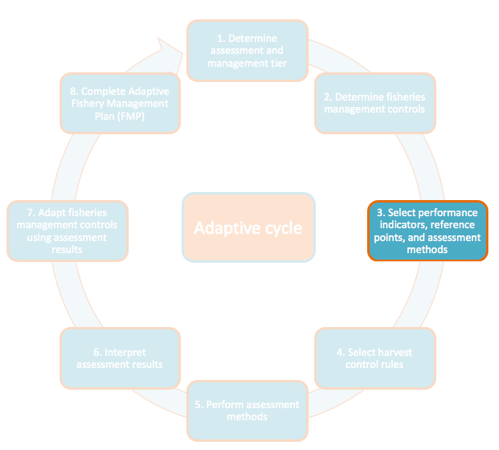
\includegraphics{myMediaFolder/media/Step3.png}
\caption{\label{fig:Step3}Step 3}
\end{figure}

Steps \protect\hyperlink{Step3a}{3a} through
\protect\hyperlink{Step3b}{3c} will guide you through selecting
appropriate performance indicators, reference points, and assessment
methods for your fishery.

While we provide best practices in these steps, it should be noted that
performance indicators and reference points are not one-size-fits-all.
They should be based on community goals for your fishery. For example,
if increased landings for food provision is a goal, you may wish to use
landings as one of your performance indicators and upward trends in
landings as a reference point. If conservation of biomass in the water
for dive tourism is a goal, you may wish to use fished:unfished density
ratio as one of your performance indicators and a high fished:unfished
density ratio as your target reference point.

\hypertarget{Step3a}{\section{Step 3a -- Select Performance
Indicators}\label{Step3a}}

Using Table \ref{tab:indicators}, select appropriate performance
indicators for your fishery. Depending on the assessment and management
tier your fishery falls under, there will be a number of options for the
indicators you may choose to select. Whenever possible, we recommend
that multiple indicators are chosen from multiple independent data
streams. This will reduce the uncertainty associated with any single
data stream and will paint a more complete picture of the fishery. Use
the specific guidance below for your tier.

\textbf{Tier 1 -- Precautionary Assessment and Management (for new sites
with less than one year of data)}

Even though limited data will be available for a Tier 1 fishery,
managers can still perform a basic qualitative fisheries assessment
using local ecological knowledge about the fishery, such as the types of
fishing gear that are currently used, changes in the fishing seasons
that have been observed over time, and changes in species composition of
landings over time. Potential performance indicators for Tier 1 are
provided in the table below, along with pros, cons, and the types of
species each indicator is appropriate for.

At a minimum, we recommended using the following performance indicators
for Tier 1:

\begin{itemize}
\item
  At least one indicator based on qualitative fisheries characterization
\item
  If available, at least one fishery-independent indicator based on
  underwater visual survey or experimental fishing
\end{itemize}

\textbf{Tier 2 -- Preliminary Adaptive Assessment and Management (for
sites with one year of data)}

Data streams in Tier 2 include those under Tier 1, as well as at least
one year of fishery-dependent data that may come from a combination of
Catch Reporting, Boat-intercept Surveys, and Fishery Dependent
Length-composition Surveys. Potential performance indicators for Tier 2
are provided in the table below, along with pros, cons, and the types of
species each indicator is appropriate for.

At a minimum, we recommended using the following performance indicators
for Tier 2:

\begin{itemize}
\item
  All indicators from Tier 1
\item
  At least one indicator based on fishery-dependent length-composition
  survey
\end{itemize}

\textbf{Tier 3 -- Multi-Indicator framework for Adaptive Assessment and
Management (for sites with more than one year of data)}

Tier 3 sites will have a time series of data available that can be used
to examine trends in multiple performance indicators in addition to
information and data described under Tiers 1 and 2. Potential Tier 3
performance indicators for each available data stream type or toolkit
output are provided in the table below, along with pros, cons, and the
types of species each indicator is appropriate for.

At a minimum, we recommended using the following performance indicators
for Tier 3:

\begin{itemize}
\item
  All indicators from Tier 2
\item
  At least one trend-based indicator that uses a time series of landings
  or CPUE data
\end{itemize}

\hypertarget{Step3b}{\section{Step 3b -- Select Reference
Points}\label{Step3b}}

During this step, select reference points for each of your chosen
performance indicators. The table below offers suggestions for generic
reference points from the literature that may be appropriate for each
performance indicator.

For every performance indicator, select both a target reference point
(TRP) as well as a limit reference point (LRP). A target reference point
is a numerical value (or trend) that indicates that the performance of
the fishery is at a desirable level; often management is geared towards
achieving or maintaining this target. This target could be a static
value chosen from the literature, or a trend in historic data (for
example, a target may be that the indicator is higher than a historic
running average). A limit reference point is a numerical value that
indicates that the performance of the fishery is unacceptable
(\emph{e.g}., severely overfished), and that management action should be
taken to improve fishery performance or population levels. Similarly,
these values may come from the literature or historic data.

When selecting reference points, we recommend the following best
practices:

\begin{itemize}
\item
  For reference points of length-based indicators and of
  fishery-independent-based indicators, we recommend using
  literature-based reference points
\item
  Whenever using reference points from literature, use reference points
  from studies of comparable species and geographic locations.
\item
  For CPUE- and landings-based indicators, we recommend using a time
  series of data to generate reference points that are based on trends
  or running averages.
\item
  If local or international scientists are available for consultation,
  discuss reference points with them to determine if they are
  appropriate for your fishery and adjust values as necessary.
\end{itemize}

Additionally, you should ensure that for each performance indicator and
assessment type that all assumptions are valid (these are listed in the
table below). The dashboard has a series of questions that will help
ensure that assumptions associated with each performance indicator and
assessment method aren't violated. Only assessment techniques that are
appropriate for your fishery will be available as options.

\section{Step 3c -- Select Assessment Methods}\label{Step3c}

During this step, select the appropriate assessment method for each of
your chosen performance indicators. The table below outlines these
options. Most performance indicators have only one associated assessment
method; however, the performance indicator of fishing mortality has
several options. There are also detailed describtions below for more
details about each specific assessment method including inputs, outputs,
and caveats.

\begin{longtable}[]{@{}llllll@{}}
\caption{\label{tab:indicators} Selecting your performance indicators,
reference points, and assessment methods}\tabularnewline
\toprule
\begin{minipage}[b]{0.14\columnwidth}\raggedright\strut
\textbf{Data stream Options}\strut
\end{minipage} & \begin{minipage}[b]{0.14\columnwidth}\raggedright\strut
\textbf{Perform ance Indicator Options}\strut
\end{minipage} & \begin{minipage}[b]{0.14\columnwidth}\raggedright\strut
\textbf{Target Reference Point}\strut
\end{minipage} & \begin{minipage}[b]{0.14\columnwidth}\raggedright\strut
\textbf{Limit Reference Point}\strut
\end{minipage} & \begin{minipage}[b]{0.14\columnwidth}\raggedright\strut
\textbf{Assessm ent Methods}\strut
\end{minipage} & \begin{minipage}[b]{0.14\columnwidth}\raggedright\strut
\textbf{Target Species}\strut
\end{minipage}\tabularnewline
\midrule
\endfirsthead
\toprule
\begin{minipage}[b]{0.14\columnwidth}\raggedright\strut
\textbf{Data stream Options}\strut
\end{minipage} & \begin{minipage}[b]{0.14\columnwidth}\raggedright\strut
\textbf{Perform ance Indicator Options}\strut
\end{minipage} & \begin{minipage}[b]{0.14\columnwidth}\raggedright\strut
\textbf{Target Reference Point}\strut
\end{minipage} & \begin{minipage}[b]{0.14\columnwidth}\raggedright\strut
\textbf{Limit Reference Point}\strut
\end{minipage} & \begin{minipage}[b]{0.14\columnwidth}\raggedright\strut
\textbf{Assessm ent Methods}\strut
\end{minipage} & \begin{minipage}[b]{0.14\columnwidth}\raggedright\strut
\textbf{Target Species}\strut
\end{minipage}\tabularnewline
\midrule
\endhead
\begin{minipage}[t]{0.14\columnwidth}\raggedright\strut
\strut
\end{minipage} & \begin{minipage}[t]{0.14\columnwidth}\raggedright\strut
\strut
\end{minipage} & \begin{minipage}[t]{0.14\columnwidth}\raggedright\strut
\strut
\end{minipage} & \begin{minipage}[t]{0.14\columnwidth}\raggedright\strut
\strut
\end{minipage} & \begin{minipage}[t]{0.14\columnwidth}\raggedright\strut
\strut
\end{minipage} & \begin{minipage}[t]{0.14\columnwidth}\raggedright\strut
\strut
\end{minipage}\tabularnewline
\begin{minipage}[t]{0.16\columnwidth}\raggedright\strut
Qualitative Survey\strut
\end{minipage} & \begin{minipage}[t]{0.16\columnwidth}\raggedright\strut
\textbf{DESTRUC TIVE FISHING GEAR}

\emph{Pros}: Relativel y easy metric to monitor using local ecologica l
knowledge

\emph{Cons}: None\strut
\end{minipage} & \begin{minipage}[t]{0.16\columnwidth}\raggedright\strut
No destructi ve fishing practices being used\strut
\end{minipage} & \begin{minipage}[t]{0.16\columnwidth}\raggedright\strut
Destructi ve fishing practices being used\strut
\end{minipage} & \begin{minipage}[t]{0.16\columnwidth}\raggedright\strut
Qualitati ve assessmen t\strut
\end{minipage} & \begin{minipage}[t]{0.16\columnwidth}\raggedright\strut
All fish and invertebr ates\strut
\end{minipage}\tabularnewline
\begin{minipage}[t]{0.16\columnwidth}\raggedright\strut
Qualitative Survey\strut
\end{minipage} & \begin{minipage}[t]{0.16\columnwidth}\raggedright\strut
\textbf{FISHING SEASON}

\emph{Pros}: Relativel y easy metric to monitor using local ecologica l
knowledge

\emph{Cons}: Changes in fishing season do not always indicate poor
fisheries performan ce; this may also result from changing environme
ntal or market condition s\strut
\end{minipage} & \begin{minipage}[t]{0.16\columnwidth}\raggedright\strut
No changes in the fishing season\strut
\end{minipage} & \begin{minipage}[t]{0.16\columnwidth}\raggedright\strut
Increased variabili ty in fishing season, or decreased fishing
season\strut
\end{minipage} & \begin{minipage}[t]{0.16\columnwidth}\raggedright\strut
Qualitati ve assessmen t\strut
\end{minipage} & \begin{minipage}[t]{0.16\columnwidth}\raggedright\strut
All fish and invertebr ates\strut
\end{minipage}\tabularnewline
\begin{minipage}[t]{0.16\columnwidth}\raggedright\strut
Qualitative Survey\strut
\end{minipage} & \begin{minipage}[t]{0.16\columnwidth}\raggedright\strut
\textbf{Target SPECIES COMPOSITI ON}

\emph{Pros}: Relativel y easy metric to monitor using local ecologica l
knowledge

\emph{Cons}: Changes in target species compositi on do not always
indicate poor fisheries performan ce; this may also result from changing
environme ntal or market condition s\strut
\end{minipage} & \begin{minipage}[t]{0.16\columnwidth}\raggedright\strut
No change in compositi on of caught species\strut
\end{minipage} & \begin{minipage}[t]{0.16\columnwidth}\raggedright\strut
Change in compositi on of caught species (fewer species, more pelagics)
or loss of major fishing targets, predators and grazers\strut
\end{minipage} & \begin{minipage}[t]{0.16\columnwidth}\raggedright\strut
Qualitati ve assessmen t\strut
\end{minipage} & \begin{minipage}[t]{0.16\columnwidth}\raggedright\strut
All fish and invertebr ates\strut
\end{minipage}\tabularnewline
\begin{minipage}[t]{0.16\columnwidth}\raggedright\strut
Qualitative Survey\strut
\end{minipage} & \begin{minipage}[t]{0.16\columnwidth}\raggedright\strut
\textbf{SPECIES VULNERABI LITY}

\emph{Pros}: Easy to interpret a species' relative vulnerabi lity to
overfishi ng relative to other species in the area/ecos ystem. This
relative vulnerabi lity score can be used to prioritiz e species for
managemen t action/as sessments

\emph{Cons}: is not an estimate of stock status\strut
\end{minipage} & \begin{minipage}[t]{0.16\columnwidth}\raggedright\strut
Low vulnerabi lity estimate (\emph{\textless{}} 2.0 PSA score); low-
medium susceptib ility and high-medi um productiv ity species are a
lower priority for managemen t action relative to species with higher
vulnerabi lity estimates (\textgreater{}2.0 PSA score)\strut
\end{minipage} & \begin{minipage}[t]{0.16\columnwidth}\raggedright\strut
High vulnerabi lity estimate (\textgreater{} 2.0 PSA score); high
susceptib ility and medium or low productiv ity species should be high
priority for managemen t action and frequent assessmen t\strut
\end{minipage} & \begin{minipage}[t]{0.16\columnwidth}\raggedright\strut
Productiv ity \& Susceptib ility Analysis\strut
\end{minipage} & \begin{minipage}[t]{0.16\columnwidth}\raggedright\strut
All fish and invertebr ates present in the ecosystem\strut
\end{minipage}\tabularnewline
\begin{minipage}[t]{0.16\columnwidth}\raggedright\strut
\emph{\textbf{Underw ater Visual Surveys or Experimen tal Fishing}
}\strut
\end{minipage} & \begin{minipage}[t]{0.16\columnwidth}\raggedright\strut
**FISHED: UNFISHED DENSITY RATIO (FOR KEY TARGET SPECIES)\emph{ }

\emph{Pros}: A Relatively quick and cheap way to assess the status of
target species.

\emph{Cons}: Assumes that a fully-fun ctioning and well-enfo rced NTZ
has been sited appropria tely with represent ative habitat, not useful
for highly mobile targets.\strut
\end{minipage} & \begin{minipage}[t]{0.16\columnwidth}\raggedright\strut
Fished:un fished density of target species \emph{\textgreater{}}
0.6\strut
\end{minipage} & \begin{minipage}[t]{0.16\columnwidth}\raggedright\strut
Fished:un fished density of target species \emph{\textless{}} 0.4\strut
\end{minipage} & \begin{minipage}[t]{0.16\columnwidth}\raggedright\strut
Density Ratio\strut
\end{minipage} & \begin{minipage}[t]{0.16\columnwidth}\raggedright\strut
Fish and invertebr ates that are habitat associate d, not a good
indicator for highly mobile targets\strut
\end{minipage}\tabularnewline
\begin{minipage}[t]{0.16\columnwidth}\raggedright\strut
\emph{\textbf{Underw ater Visual Surveys or Experimen tal Fishing}
}\strut
\end{minipage} & \begin{minipage}[t]{0.16\columnwidth}\raggedright\strut
\textbf{FISHED: UNFISHED BIOMASS RATIO (CORAL REEF THRESHOLD AGGREGATE D
ACROSS SPECIES) -- Only for Underwate r Visual Surveys}

\emph{Pros}: Provides an estimate of ecosystem status and capacity to
support fishing, useful for setting precautio nary managemen t to meet
EBFM goals.

\emph{Cons}: Assumes that a fully-fun ctioning and well-enfo rced NTZ
has been sited appropria tely with represent ative habitat, not useful
for highly mobile targets. Assumes NTZ are represent ative of historica
l, unfished biomass.\strut
\end{minipage} & \begin{minipage}[t]{0.16\columnwidth}\raggedright\strut
Fished:un fished biomass ratio \emph{\textgreater{}} 0.5\strut
\end{minipage} & \begin{minipage}[t]{0.16\columnwidth}\raggedright\strut
Fished:un fished biomass ratio \emph{\textless{}} 0.25\strut
\end{minipage} & \begin{minipage}[t]{0.16\columnwidth}\raggedright\strut
Coral Reef Threshold s\strut
\end{minipage} & \begin{minipage}[t]{0.16\columnwidth}\raggedright\strut
Multi-spe cies finfish fishery\strut
\end{minipage}\tabularnewline
\begin{minipage}[t]{0.16\columnwidth}\raggedright\strut
\emph{\textbf{Underw ater Visual Surveys or Experimen tal Fishing}
}\strut
\end{minipage} & \begin{minipage}[t]{0.16\columnwidth}\raggedright\strut
\textbf{AVERAGE LENGTH}

\emph{Pros}: Easy, cheap metric to assess changes in the status of a
fishery

\emph{Cons}: Does not capture selectivi ty of the fishery, or is fishing
is prosecute d in nursery grounds\strut
\end{minipage} & \begin{minipage}[t]{0.16\columnwidth}\raggedright\strut
Decrease in the size of unfished individua ls outside of the NTZ, in
compariso n to previous years\strut
\end{minipage} & \begin{minipage}[t]{0.16\columnwidth}\raggedright\strut
Rapid decrease in the size of individua ls outside of the NTZ, in
compariso n to previous years\strut
\end{minipage} & \begin{minipage}[t]{0.16\columnwidth}\raggedright\strut
Average Length\strut
\end{minipage} & \begin{minipage}[t]{0.16\columnwidth}\raggedright\strut
Multi-spe cies, habitat associate d targets, not a good indicator for
highly mobile targets\strut
\end{minipage}\tabularnewline
\begin{minipage}[t]{0.16\columnwidth}\raggedright\strut
\textbf{\emph{Fisher y Dependent Length-Co mposition Survey}}\strut
\end{minipage} & \begin{minipage}[t]{0.16\columnwidth}\raggedright\strut
\textbf{FISHING MORTALITY DIVIDED BY NATURAL MORTALITY (F/M)}

\emph{Pros}: Mortality rates are critical for determini ng abundance of
fish populatio ns

\emph{Cons}: All of the models assume equilibri um condition s. Most of
these methods only reflect fish that have recruited to a fishery and
does not reflect the full age structure of a stock.\strut
\end{minipage} & \begin{minipage}[t]{0.16\columnwidth}\raggedright\strut
F/M \textless{}1 (F is fishing mortality , M is natural mortality
)\strut
\end{minipage} & \begin{minipage}[t]{0.16\columnwidth}\raggedright\strut
F=2M\strut
\end{minipage} & \begin{minipage}[t]{0.16\columnwidth}\raggedright\strut
Catch Curve or LBAR\strut
\end{minipage} & \begin{minipage}[t]{0.16\columnwidth}\raggedright\strut
Finfish (groupers , snapper, grunts, etc.), and invertebr ates with
indetermi nate growth (lobsters , crabs). Use with care for targets that
have determini stic growth and episodic recruitme nt.\strut
\end{minipage}\tabularnewline
\begin{minipage}[t]{0.16\columnwidth}\raggedright\strut
\textbf{\emph{Fisher y Dependent Length-Co mposition Survey}}\strut
\end{minipage} & \begin{minipage}[t]{0.16\columnwidth}\raggedright\strut
\textbf{SPAWNIN G POTENTIAL RATIO (SPR)}

\emph{Pros}: can be used with fishery independe nt and dependent data.

\emph{Cons}: Assumes equilibri um condition s and an index based on the
early life history of a fish\strut
\end{minipage} & \begin{minipage}[t]{0.16\columnwidth}\raggedright\strut
\emph{slow growing species, M/k\textless{} 1 (grouper) SPR
}\textgreater{}\emph{ 40\% (M is natural mortality , k is von Bertalanf
fy growth rate)}

\emph{fast growing species, M/k \textgreater{}1 (lobster) SPR
=20\%}\strut
\end{minipage} & \begin{minipage}[t]{0.16\columnwidth}\raggedright\strut
\emph{slow growing species, M/k\textless{} 1 (grouper) SPR
\textless{}40\%}

\emph{fast growing species, M/k \textgreater{}1 (lobster) SPR
\textless{}20\%}\strut
\end{minipage} & \begin{minipage}[t]{0.16\columnwidth}\raggedright\strut
Length-ba sed SPR (LBSPR)\strut
\end{minipage} & \begin{minipage}[t]{0.16\columnwidth}\raggedright\strut
Finfish (groupers , snapper, grunts, etc.), and invertebr ates with
indetermi nate

growth (lobsters , crabs). Use with care for targets that have determini
stic growth and episodic recruitme nt.\strut
\end{minipage}\tabularnewline
\begin{minipage}[t]{0.16\columnwidth}\raggedright\strut
\textbf{\emph{Fisher y Dependent Length-Co mposition Survey}}\strut
\end{minipage} & \begin{minipage}[t]{0.16\columnwidth}\raggedright\strut
\textbf{AVERAGE LENGTH}

\emph{Pros}: Easy, cheap metric to assess changes in the status of a
fishery when stratifie d across sampling unit (gear, efforts, fishing
zone)

\emph{Cons}: With little to no historica l informati on on the length of
the catch or with no informati on on gear selectivi ty, the average
length could bias the expected potential size distribut ion.\strut
\end{minipage} & \begin{minipage}[t]{0.16\columnwidth}\raggedright\strut
Increase in average length\strut
\end{minipage} & \begin{minipage}[t]{0.16\columnwidth}\raggedright\strut
Decrease in average length or mature adults\strut
\end{minipage} & \begin{minipage}[t]{0.16\columnwidth}\raggedright\strut
Average Length\strut
\end{minipage} & \begin{minipage}[t]{0.16\columnwidth}\raggedright\strut
All targets, especiall y nearshore targets. In an ideal scenario an
historic record of average length would be used to compare current to
past estimates .\strut
\end{minipage}\tabularnewline
\begin{minipage}[t]{0.16\columnwidth}\raggedright\strut
\textbf{\emph{Fisher y Dependent Length-Co mposition Survey}}\strut
\end{minipage} & \begin{minipage}[t]{0.16\columnwidth}\raggedright\strut
\textbf{FROESE INDICATOR S}

\emph{Pros}: Proven estimate of the status of the stock, in compariso n
to sustainab ility reference points

\emph{Cons}: Does not contribut e to biomass sustainab ility reference
points\strut
\end{minipage} & \begin{minipage}[t]{0.16\columnwidth}\raggedright\strut
Spawning biomass above reference point\strut
\end{minipage} & \begin{minipage}[t]{0.16\columnwidth}\raggedright\strut
Spawning biomass below reference point and fish are small and
immature\strut
\end{minipage} & \begin{minipage}[t]{0.16\columnwidth}\raggedright\strut
Froese Sustainab ility Indicator s\strut
\end{minipage} & \begin{minipage}[t]{0.16\columnwidth}\raggedright\strut
All fish and invertebr ate target with known length-ag e/maturit y
relations hips\strut
\end{minipage}\tabularnewline
\begin{minipage}[t]{0.16\columnwidth}\raggedright\strut
\textbf{\emph{Indivi dual Catch Reporting System \& Boat Intercept
/Landing Site Survey}}\strut
\end{minipage} & \begin{minipage}[t]{0.16\columnwidth}\raggedright\strut
\textbf{CPUE}

\emph{Pros}: Can be used to infer populatio n trends of an exploited
stock. Standardi zed time series of CPUE are often regarded as indices
of abundance .

\emph{Cons}: Seldom proportio nal to abundance history and an entire
geographi c range. Can be skewed, depending on sampling regime. May have
species-s pecific biases.\strut
\end{minipage} & \begin{minipage}[t]{0.16\columnwidth}\raggedright\strut
Stable CPUE\strut
\end{minipage} & \begin{minipage}[t]{0.16\columnwidth}\raggedright\strut
Rapidly Decreasin g CPUE, previous year or in compariso n to running
average\strut
\end{minipage} & \begin{minipage}[t]{0.16\columnwidth}\raggedright\strut
Catch Trends\strut
\end{minipage} & \begin{minipage}[t]{0.16\columnwidth}\raggedright\strut
All targets that do not have high selectivi ty of habitat stratific
ation.\strut
\end{minipage}\tabularnewline
\begin{minipage}[t]{0.16\columnwidth}\raggedright\strut
\textbf{\emph{Indivi dual Catch Reporting System \& Boat Intercept
/Landing Site Survey}}\strut
\end{minipage} & \begin{minipage}[t]{0.16\columnwidth}\raggedright\strut
**TOTAL LANDINGS\emph{ }

\emph{Pros}: when sampling is stratifie d, can provide an estimate of
abundance

\emph{Cons}: seldom proportio nal to abundance history and an entire
geographi c range, because of fishing location biases and lack of
sampling stratific ation\strut
\end{minipage} & \begin{minipage}[t]{0.16\columnwidth}\raggedright\strut
Increase in Total Landing\strut
\end{minipage} & \begin{minipage}[t]{0.16\columnwidth}\raggedright\strut
Rapidly Decreasin g Total Landings, previous year or in compariso n to
running average\strut
\end{minipage} & \begin{minipage}[t]{0.16\columnwidth}\raggedright\strut
Catch Trends\strut
\end{minipage} & \begin{minipage}[t]{0.16\columnwidth}\raggedright\strut
All targets that do not have high selectivi ty of habitat stratific
ation.\strut
\end{minipage}\tabularnewline
\bottomrule
\end{longtable}

\section{Assessment Method
Descriptions}\label{assessment-method-descriptions}

\textbf{\emph{Fishery Independent-Data}}

\textbf{\emph{Coral Reef Thresholds}}

\begin{itemize}
\tightlist
\item
  \textbf{Description}: This method uses the ratio of total fish biomass
  inside a no-take-zone (NTZ) to the total fish biomass outside the NTZ.
  For some ecosystems, including coral reefs, recent studies show the
  existence of quantitative thresholds associated with fish densities
  (measured in kg/ha). Below these thresholds, ecosystems change from
  desirable (e.g., high coral cover) to less desirable states (e.g.,
  dominated by algae) that produce fewer ecosystem services. Fisheries
  in ecosystems with documented fishing thresholds can be managed to
  remain above these limits, reducing the risk of system collapse. At
  the moment, thresholds have been documented for coral reefs in the
  Indian Ocean (McClanahan et al. 2011) and the Caribbean Sea (Karr et
  al. 2014). Biomass of fished populations and unfished populations can
  be measured with experimental fishing or visual surveys, and the
  resulting ratio of biomass from these surveys can then be compared to
  the threshold limits. Comparing this ratio to a target ratio defined
  in Karr et al. 2015, fishing pressure can be adjusted accordingly to
  maintain the fish biomass outside of a NTZ above the 0.5
  \emph{B\textsubscript{MSY}} (Biomass maximum multi-species sustainable
  yield) target.
\end{itemize}

\textbf{Inputs:}

\begin{itemize}
\tightlist
\item
  Estimate of total fish biomass inside and outside of NTZ
\end{itemize}

\textbf{Outputs:}

\begin{itemize}
\tightlist
\item
  Ratio of fish biomass outside the NTZ to the biomass inside the NTZ
\end{itemize}

\textbf{How this can be used by management:}

\begin{itemize}
\item
  Integrates many species into an ecosystem community metric
\item
  Provides a reference direction of overall fishing mortality for all
  species
\item
  Provides precautionary estimate of current status of ecosystem that
  supports the fishery
\end{itemize}

\textbf{Input Sensitivities:}

\begin{itemize}
\tightlist
\item
  Assumes no-take reserves are representative of historical, unfished
  biomass
\end{itemize}

\textbf{Caveats:}

\begin{itemize}
\tightlist
\item
  This method assumes that a fully-functioning and well-enforced NTZ has
  been sited appropriately with representative habitat inside and
  outside of the NTZ, and been in place long enough for the population
  living inside the NTZ to be a proxy for an un-fished population.
\end{itemize}

\textbf{\emph{Fished:Unfished Density Ratio (DR)}}

\textbf{Description:} The DR uses fishery-independent data comparing
ratios of density, average length density of a specific life stage
(immature, mature adults, optimal size or mega-spawners), or CPUE
outside to inside of no-take zones (NTZs). Babcock \& MacCall (2011)
provide a clear analysis of the use of density ratio (DR) assessment
methods. The DR's control rule adjusts fishing pressure according to the
distance of the ratio of density outside to inside of the NTZ from a
pre-specified target ratio. One drawback of the density ratio is that in
situations where populations inside and outside the reserves both crash,
the ratio would remain the same and indicate that fishing can commence.
In the DR analysis, we modified the DR control rule to account for this
dynamic. The adjustment is scaled by the overall health of the
population inside the NTZ, measured as the density inside of the NTZ
relative to the historic maximum density recorded in the NTZ.

\textbf{Inputs: }

\begin{itemize}
\item
  Density (or length by species) data inside and outside the NTZ
  (preferably collected in the same manner)
\item
  Historical maximum density inside the NTZ
\end{itemize}

\textbf{Outputs: }

\begin{itemize}
\tightlist
\item
  Ratio of fish density outside the NTZ to the density inside the NTZ
\end{itemize}

\textbf{How this can be used by management:}

\begin{itemize}
\item
  Stakeholders set a management target DR
\item
  This DR target ratio is compared to the ratio from assessment
\item
  Effort is adjusted based on how far apart these values are
\end{itemize}

\textbf{Input Sensitivities: }

\begin{itemize}
\tightlist
\item
  Assumes historical maximum density inside the NTZ
\end{itemize}

\textbf{Caveats:}

\begin{itemize}
\item
  This method assumes that a fully-functioning and well-enforced NTZ has
  been sited appropriately with representative habitat inside and
  outside of the NTZ, and has been in place long enough for the
  population living inside the NTZ to be a proxy for an un-fished
  population.

  \begin{itemize}
  \tightlist
  \item
    \emph{Implication}: May be less accurate for highly-mobile species
    that do not remain exclusively inside the NTZ such as snapper, tuna
    and mackerel.
  \end{itemize}
\item
  Time trends in this data can be difficult to interpret if densities
  inside the MPA are changing rapidly
\end{itemize}

\textbf{\emph{No-take zone catch-curve (Catch Curve)}}

\textbf{Description:} This method utilizes length-frequency data (fish
lengths) from inside and outside a NTZ to compare the slope of the
right-hand side of the log transformed age-frequency histogram from
inside the NTZ (an estimate of natural mortality (\emph{M})) to the
slope of the log transformed age-frequency histogram outside the NTZ (an
estimate of total mortality (\emph{Z})). Fishing mortality (\emph{F})
can then be calculated based on the difference between these two
(\emph{F} = \emph{Z} -- \emph{M}).

\textbf{Inputs:}

\begin{itemize}
\item
  Length-frequency data inside and outside NTZ (preferably collected in
  the same manner)
\item
  Life history parameters (growth parameters)
\item
  How many years the NTZ has been established and well-enforced
\item
  Information on the sizes of fish preferred by the fishery
\end{itemize}

\textbf{Outputs}

\begin{itemize}
\tightlist
\item
  An estimate of fishing mortality (\emph{F})
\end{itemize}

\textbf{How this can be used by management :}

\begin{itemize}
\item
  Stakeholders set management target F/M based on community objectives
  and thresholds of risk
\item
  Target \emph{F}/\emph{M} is compared with \emph{F}/\emph{M} from
  assessment
\item
  Effort is adjusted through harvest control rules based on how far
  apart these values are
\end{itemize}

\textbf{Input Sensitivities: }

\begin{itemize}
\item
  Accuracy of individual fish length measurements
\item
  Accuracy of length-at-age relationships (\emph{Von Bertanalffy growth
  parameters}
\item
  Correcting fitting of the curve (sensitive to estimates of NTZ age,
  preferred fish size)
\end{itemize}

\textbf{Caveats}:

\begin{itemize}
\item
  This method assumes that a NTZ has been sited appropriately,
  well-enforced, and been in place long enough for the population living
  inside the NTZ to be a proxy for an un-fished population

  \begin{itemize}
  \tightlist
  \item
    \emph{Implication}: May be less accurate for highly-mobile species
    that do not remain exclusively inside the NTZ, such as snapper, tuna
    and mackerel
  \end{itemize}
\item
  This method depends on reliably tracking population size structure
  changes, thus may be less accurate with small, fast-growing species
\end{itemize}

\textbf{\emph{Fishery-Dependent Data}}

\textbf{\emph{Trends Analyses}}

\textbf{Description:} This method uses catch data to compare total
catch, average catch, CPUE, and/or abundance between years of interests.
Comparisons can be derived for sequential years, or as a running average
between historical trends. Additionally, comparisons can be made across
all species or by species of interest.

\textbf{Inputs:}

\begin{itemize}
\item
  Total catch for more than one year
\item
  Catch-Per-Unit-Effort (CPUE) for more than one year
\item
  Abundance of the catch for more than one year
\item
  Length-frequency of the catch for more than one year
\end{itemize}

\textbf{Outputs:}

\begin{itemize}
\item
  Total catch and trends in total catch
\item
  CPUE and trends in CPUE
\item
  Abundance and trends in abundance
\item
  Average length and trends in average length
\end{itemize}

\textbf{How this can be used by management:}

\begin{itemize}
\item
  Catch trends can support the interpretation of other analyses, for
  example of fishing morality of spawning potential ratio (SPR).
\item
  Understanding how the trends in catch fluctuate from one year to next
  or in comparison to the historic trends is essential to use catch
  trends for management.
\end{itemize}

\textbf{Input Sensitivities:}

\begin{itemize}
\tightlist
\item
  It can be difficult to attribute a change in catch to a corresponding
  increase or decrease in biomass. Therefore, seeing an increase in
  catch could provide a false sense of security. Inferring stock status
  from catch statistics
\end{itemize}

\textbf{Caveats:}

\begin{itemize}
\item
  This method depends on reliably tracking the total catch
\item
  For example, raw CPUE is seldom proportional to abundance over a
  \textgreater{} whole exploitation history and an entire geographic
  range, because \textgreater{} numerous factors affect catch rates.
\end{itemize}

\textbf{\emph{Catch Curve}}

\textbf{Description:} This method utilizes length-frequency data (fish
lengths) to estimate the fishing mortality affecting the fished
population. Total fishing mortality (\emph{Z}) is estimated using the
slope of the log transformed age-frequency histogram. Fishing mortality
can then be calculated based on the difference between total fishing
mortality and natural mortality (\emph{F} = \emph{Z} -- \emph{M}).
Estimates of \emph{M} can come from the literature.

\textbf{Inputs:}

\begin{itemize}
\item
  Length-frequency data
\item
  Life history parameters (growth parameters)
\end{itemize}

\textbf{Outputs: }

\begin{itemize}
\tightlist
\item
  An estimate of fishing mortality
\end{itemize}

\textbf{How this can be used by management:}

\begin{itemize}
\item
  Stakeholders set management target \emph{F}/\emph{M} based on
  community objectives and thresholds of risk
\item
  Target \emph{F}/\emph{M} is compared with \emph{F}/\emph{M} from
  assessment
\item
  Effort is adjusted through harvest control rules based on how far
  apart these values are
\end{itemize}

\textbf{Input Sensitivities: }

\begin{itemize}
\item
  Accuracy of individual fish length measurements
\item
  Accuracy of length-at-age relationships (Von Bertalanffy growth
  parameters)
\item
  Correcting fitting of the curve (i.e., preferred fish size)
\end{itemize}

\textbf{Caveats:}

\begin{itemize}
\tightlist
\item
  This method depends on reliably tracking population size structure
  \textgreater{} changes, thus may be less accurate for small,
  fast-growing species
\end{itemize}

\textbf{\emph{Froese Sustainability Indicators}}

\textbf{Description:} This method uses the length-frequency of the catch
and life history growth parameters to estimate the distribution of life
stages in the catch (Froese 2004, Cope and Punt 2009), and subsequently
whether or not the catch is sustainable.

\textbf{Inputs: }

\begin{itemize}
\item
  Length-frequency of the catch
\item
  Length at maturity
\item
  Natural mortality
\item
  Von Bertalanffy growth parameters
\end{itemize}

\textbf{Outputs: }

\begin{itemize}
\item
  This method first calculates three metrics of fisheries
  sustainability:

  \begin{itemize}
  \item
    (i) percentage of mature fish in catch, with 100\% as target;
  \item
    (ii) percent of specimens with optimum length in catch
    (\emph{L\textsubscript{opt}}), with 100\% as target;
  \item
    and (iii) percentage of `mega-spawners' in catch
  \end{itemize}
\item
  Using these three metrics and the life history parameters, the method
  next uses a decision tree to determine whether or not spawning biomass
  is greater or less than a sustainable target reference point.
\end{itemize}

\textbf{How this can be used by management:}

\begin{itemize}
\tightlist
\item
  By fishing at \emph{L\textsubscript{opt}} or by fishing matural
  individuals with the ``spawn-at-least-once'' principle, in conjunction
  with the protection of \emph{megaspawners}, sustainability of the
  fishery can be maintained.
\item
  If this method determines spawning biomass is less than the TRP,
  adjustments in management may be necessary
\end{itemize}

\textbf{Input Sensitivities:}

\begin{itemize}
\item
  Accuracy of individual fish length measurements
\item
  Accuracy of length at maturity
\item
  Selectivity
\end{itemize}

\textbf{Caveats:}

\begin{itemize}
\item
  This method depends on reliably tracking population size structure
  \textgreater{} changes

  \begin{itemize}
  \tightlist
  \item
    Implication: May be less accurate with small, fast-growing
    \textgreater{} species
  \end{itemize}
\end{itemize}

\textbf{\emph{Mean Length (L\textsubscript{bar})}}

\textbf{Description:} This method uses fishery-dependent or independent
length-frequency data. \emph{L\textsubscript{bar}} uses the minimum and
maximum fished sizes, and the average length of the fish within the
fished sizes from a fished population, along with growth parameters. In
the Ault et al. 2005 model, \emph{L\textsubscript{bar}} provides an
estimate of fishing mortality (\emph{F}) that can be compared to an
estimate of natural mortality (\emph{M}). Intuitively, increasing
fishing pressure will often cause decreasing average length.

\textbf{Inputs: }

\begin{itemize}
\item
  Fishery-dependent or fishery-independent length-frequency data of
  fished population
\item
  Life history parameters, growth parameters, and natural mortality
  (\emph{M})
\item
  Information on the sizes of fish preferred by the fishery
\end{itemize}

\textbf{Outputs}:

\begin{itemize}
\tightlist
\item
  An estimate of fishing mortality (\emph{F})
\end{itemize}

\textbf{How this can be used by management:}

\begin{itemize}
\item
  Stakeholders set management target \emph{F}/\emph{M} based on
  community objectives and thresholds of risk
\item
  Target \emph{F}/\emph{M} is compared with \emph{F}/\emph{M} from
  assessment
\item
  Effort is adjusted based on how far apart \emph{F}/\emph{M} from the
  assessment is from the \emph{F}/\emph{M}
\end{itemize}

\textbf{Input Sensitivities: }

\begin{itemize}
\item
  Estimate of \emph{M} and growth parameters
\item
  Accuracy of individual fish length measurements
\end{itemize}

\textbf{Caveats: }

\begin{itemize}
\item
  This method depends on reliably tracking population size structure
  \textgreater{} changes

  \begin{itemize}
  \tightlist
  \item
    Implication: May be less accurate with small, fast-growing
    \textgreater{} species
  \end{itemize}
\item
  \emph{M} is assumed to be known, which often it is not
\item
  Assumes equilibrium
\item
  This model is less reliable when mean fish length is very low
\end{itemize}

\textbf{\emph{Mean Weight}}

\textbf{Description:} This method can use fishery-dependent or
independent weight-frequency data to estimate fishing mortality
(\emph{F}) when no size structure data is available. This method
requires the von Bertalanffy growth function, as well as the
length-weight relationship and the natural mortality (\emph{M}). In this
method, we construct a Yield-Per-Recruit (YPR) model, which allows us to
estimate the theoretical age and weight structure of the population at
any size. Similar to Mean Length (\emph{L\textsubscript{bar}}), Mean
Weight provides an estimate of \emph{F} that can be compared to an
estimate of \emph{M}. Intuitively, increasing fishing pressure will
often cause decreasing average weight and/ or length.

\textbf{Inputs: }

\begin{itemize}
\item
  Fishery-dependent or fishery-independent weight-frequency data
\item
  Life history parameters, growth parameters, natural mortality
  (\emph{M})
\item
  Information on the sizes of fish preferred by the fishery
\end{itemize}

\textbf{Outputs}:

\begin{itemize}
\tightlist
\item
  An estimate of fishing mortality (\emph{F})
\end{itemize}

\textbf{How this can be used by management: }

\begin{itemize}
\item
  Stakeholders set management target \emph{F}/\emph{M} based on
  community objectives and thresholds of risk
\item
  Target \emph{F}/\emph{M} is compared with \emph{F}/\emph{M} from
  assessment
\item
  Effort is adjusted based on how far apart these values are
\end{itemize}

\textbf{Input Sensitivities: }

\begin{itemize}
\item
  Estimate of \emph{M} and growth parameters
\item
  Accuracy of individual fish weight measurements
\item
  Accuracy of length-weight relationship
\end{itemize}

\textbf{Caveats: }

\begin{itemize}
\item
  This method depends on reliably tracking population size structure
  changes

  \begin{itemize}
  \tightlist
  \item
    Implication: May be less accurate for small, fast-growing species
  \end{itemize}
\item
  \emph{M} is assumed to be known, which often it is not
\item
  Assumes equilibrium
\item
  This model is less reliable when mean fish weight is very low
\end{itemize}

\textbf{\emph{Bounded mean length mortality estimator}}

\textbf{Description:} A modification of the Mean Length
(\emph{L\textsubscript{bar}}) method (Ehrhardt et al. 1992). Does not
assume that fishing mortality has been constant over the life span of
the fish being assessed, it takes into account the time since a
management change, and restricts the data used for this analysis to
those fish which have recruited to the fishery during this time period.

\textbf{Inputs:}

\begin{itemize}
\item
  Length-frequency of the catch, since management change
\item
  Mean asymptotic length (cm) of the von Bertalanffy growth equation
\item
  \emph{L\textsubscript{λ}}, the age at \emph{L\textsubscript{c}} (using
  the von Bertalanffy equation) and adding the number of years since a
  known harvest rate policy change, then converting back to length
\item
  \emph{L\textsubscript{bar}} is the mean length of fish between
  \emph{L\textsubscript{c}} and \emph{L\textsubscript{λ}}.
\end{itemize}

\textbf{Outputs:}

\begin{itemize}
\tightlist
\item
  An estimate of fishing mortality (\emph{F})
\end{itemize}

\textbf{How this can be used by management: }

\begin{itemize}
\item
  Stakeholders set management target \emph{F}/\emph{M} based on
  community objectives and thresholds of risk
\item
  Target \emph{F}/\emph{M} is compared with \emph{F}/\emph{M} from
  assessment
\item
  Effort is adjusted based on how far apart these values are
\end{itemize}

\textbf{Input Sensitivities: }

\begin{itemize}
\item
  Estimate of \emph{M} and growth parameters
\item
  Accuracy of individual fish length measurements
\end{itemize}

\textbf{Caveats: }

\begin{itemize}
\item
  This method depends on reliably tracking population size structure
  changes

  \begin{itemize}
  \tightlist
  \item
    Implication: May be less accurate for small, fast-growing species
  \end{itemize}
\item
  \emph{M} is assumed to be known, which often it is not
\item
  Assumes equilibrium
\item
  This model is less reliable when mean fish length is very low
\end{itemize}

\textbf{\emph{Length-based Spawning Potential Ratio (LBSPR)}}

\textbf{Description:} Length-based Spawning Potential Ratio (LBSPR)
method uses length-frequency data from a fished population to calculate
the spawning potential ratio (SPR) of a fishery (Hordyk et al. 2014).
This method is based on the concept that the equilibrium unfished size
structure of a population depends on the average maximum size attained
and the ratio of the rate of natural mortality (\emph{M}) to the
individual growth rate (\emph{K}; Prince et al. 2014). SPR is a measure
of current egg production relative to maximum possible production at
un-fished levels. Un-fished egg production is estimated using the
natural mortality (\emph{M}), Von Bertanaffy (\emph{VBK}) growth
parameters, age at first maturity, and fecundity at age. The fished SPR
is calculated using the same parameters, along with estimates of the
fishing mortality rate (\emph{F}), and the sizes of fish selected by the
fishery. By comparing the estimated current SPR with a target SPR
defined by stakeholders, a harvest control rule can be used to adjust
fisheries management controls accordingly.

\textbf{Inputs}:

\begin{itemize}
\tightlist
\item
  Length-frequency data from a fished population
\end{itemize}

\begin{itemize}
\item
  Gear selectivity
\item
  Life history parameters (fecundity, \emph{VBK} parameters, natural
  mortality, age-at-maturity, length at age relationships)
\end{itemize}

\textbf{Outputs:}

\begin{itemize}
\tightlist
\item
  SPR of target species
\end{itemize}

\textbf{How this can be used by management: }

\begin{itemize}
\item
  Stakeholders set management target SPR
\item
  Target SPR is compared to SPR from assessment
\item
  Effort is adjusted based on how far apart these values are
\end{itemize}

\textbf{Input Sensitivities: }

\begin{itemize}
\item
  Accuracy of individual fish length measurements
\item
  Representativeness of the length data
\item
  Accuracy of life history information, particularly growth and maturity
  parameters
\end{itemize}

\textbf{Caveats:}

\begin{itemize}
\item
  This method is dependent on reliably tracking changes in population
  size structure

  \begin{itemize}
  \tightlist
  \item
    \emph{Implication}: May be less accurate for small, fast-growing
    species, such as surgeonfish, scad and spinefoot rabbit fish
  \end{itemize}
\item
  Assumes the fishery is equilibrium and that conditions are relatively
  stable (environmental conditions, fishing pressure, stock status,
  etc.)
\item
  This method is less accurate if fishing pressure has been changing
  dramatically year to year
\item
  This method is less effective for species with highly variable
  recruitment (addition of juveniles to the population) such as lobster
\end{itemize}

\hypertarget{Step4}{\chapter{Step 4 -- Define Harvest Control
Rules}\label{Step4}}

\emph{How should FMCs be adjusted according to the performance
indicators of the fishery?}

\begin{figure}
\centering
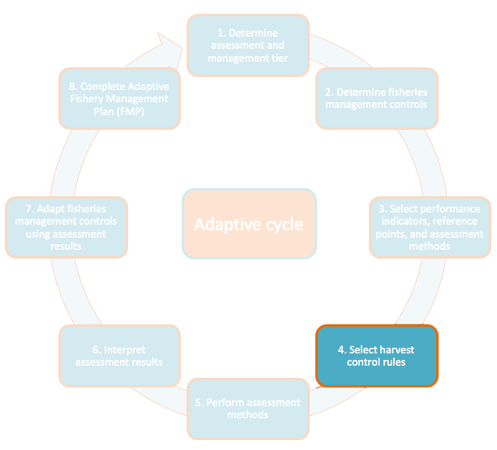
\includegraphics{myMediaFolder/media/Step4.png}
\caption{\label{fig:Step4}Step 4}
\end{figure}

\emph{Harvest Control Rules (HCRs)} will be used to adjust FMCs
according to where the fishery's performance indicators fall relative to
their reference points. The HCR may specify some combination of
adjustments to the FMCs that is expected to move the performance
indicator towards the target reference point, and away from the
\emph{limit reference point}\textbf{,} therefore improving the
performance of the fishery. While we provide guidance to define HCRs, it
should be noted that HCRs should be based on realistic compliance and
enforcement concerns and address community goals for your fishery (more
guidance is provided in Step 4b).

It is important for stakeholders and managers to agree on the suite of
HCRs in a safe and neutral setting before any management decisions need
to be made. This can help improve compliance by ensuring management
responses are objective, consistent, transparent, and appropriate.
Therefore, it is important to identify all foreseeable possible
scenarios that could occur in the fishery and create corresponding HCRs
for each scenario.

\section{Step 4a -- Define General Harvest Control Rules for All
Possible
Interpretations}\label{step-4a-define-general-harvest-control-rules-for-all-possible-interpretations}

During this step, you will define general harvest control rules (for
example, if the performance indicator is below the target reference
point, reduce the total allowable catch). In the following step, you
will add specificity to your harvest control rules (for example, if the
performance indicator is 20\% below the target reference point, reduce
the total allowable catch by 20\%). It is important that you define a
HCR for every foreseeable interpretation so that management responses
can be transparent and objective when the time comes to implement them.

Use Tabls \ref{tab:hcrs-1}, \ref{tab:hcrs-2}, and \ref{tab:hcrs-3} as
the framework for defining your general HCRs. The three tables contain
the performance indicators that are associated with each tier and
suggest HCRs from the literature. For each performance indicator and
assessment result, the table lists a number of potential interpretations
and corresponding HCRs. This table provides some examples, but is by no
means comprehensive or prescriptive -- it is illustrative only.

Each row also has a traffic light indicator that describes if a
management response is necessary:

\begin{itemize}
\item
  Green indicates that either no management response is necessary, or
  management could be even less restrictive.
\item
  Yellow indicates that a precautionary or more restrictive management
  response should be implemented.
\item
  Red indicates that the fishery should be closed and a fishery recovery
  plan implemented.
\end{itemize}

\section{Step 4b -- Add Specificity to Harvest Control
Rules}\label{step-4b-add-specificity-to-harvest-control-rules}

During this step, you will add specificity to your HCRs (for example, if
the performance indicator is 20\% below the target reference point,
reduce the total allowable catch by 20\%). Be as specific as possible
when defining the magnitude to which FMCs should be adjusted given the
fishery's performance indicator.

The magnitude that a HCR should adjust your FMC(s) will depend on:

\begin{enumerate}
\def\labelenumi{\arabic{enumi}.}
\item
  Productivity (life history) of the target species

  \begin{enumerate}
  \def\labelenumii{\alph{enumii}.}
  \item
    Productivity of key target species is an output of the FLAGS
    toolkit. This information may either come from a PSA result or a
    more data-limited qualitative approach for assessing species
    productivity.
  \item
    Species with low productivity will require higher, more restrictive
    levels of response when changes are necessary; species with higher
    productivity will require lower levels of response when changes are
    necessary
  \end{enumerate}
\item
  Likelihood of compliance
\item
  Social and political feasibility
\item
  Enforcement capacity
\item
  Level of uncertainty with data and the estimation of performance
  indicators,

  \begin{enumerate}
  \def\labelenumii{\alph{enumii}.}
  \tightlist
  \item
    The more uncertain you are, the more precautionary you may want to
    make your management
  \end{enumerate}
\item
  Risk tolerance.

  \begin{enumerate}
  \def\labelenumii{\alph{enumii}.}
  \tightlist
  \item
    Communities with higher risk tolerance may choose to be more lenient
    when choosing HCRs, while communities with lower risk tolerance may
    choose more restrictive HCRs to be more precautionary in the face of
    changing and uncertain conditions.
  \end{enumerate}
\end{enumerate}

You should consult any existing social survey data when setting HCRs.
KAP data will provide an indication as to individual attitudes towards
fishery management in your community. Social survey data will provide
context as to how dependent the community is on the fishery and how
changes in fisheries management controls may affect their livelihoods.
Additionally, any existing enforcement data should be consulted to gain
a better sense for the likelihood of compliance with any new
regulations.

You should also consider the size of any NTZ when setting HCRs. Sites
with a small NTZ relative to the size of the fishery may wish the
exercise more precaution by setting more restrictive HCRs (i.e., if
indicators are interpreted to mean poor fisheries performance, make more
drastic adjustments to the FMCs). Sites with an NTZ that is not placed
explicitly in areas that protect critical habitat may also wish to
exercise more precaution with stricter HCRs. Sites with larger NTZs that
protect a significant portion of critical habitat could be more lenient
in their HCRs. Often, large and well-placed NTZs can act as a buffer
against uncertainty and variability. By completely restricting access to
a certain portion of the stock, marine reserves are analogous to an
emergency savings account. Protecting a fraction of a fish stock in
reserves reduces the risk of overfishing and the chance of stock
collapse in the long term. Displaced fishing effort and unintended
consequences resulting after implementation of a reserve can be
mitigated when effective FMCs are in place outside of the reserve. When
harvest levels are appropriately controlled a spillover of biomass from
marine reserves to the adjacent fishery may occur that can benefit
fisheries.

\begin{longtable}[]{@{}lllll@{}}
\caption{\label{tab:hcrs-1} Indicators for Tier 1: Possible interpretations,
management implications, and suggested harvest control
rules}\tabularnewline
\toprule
\begin{minipage}[b]{0.17\columnwidth}\raggedright\strut
\textbf{Performan ce Indicator}\strut
\end{minipage} & \begin{minipage}[b]{0.17\columnwidth}\raggedright\strut
\textbf{Assessmen t Result}\strut
\end{minipage} & \begin{minipage}[b]{0.17\columnwidth}\raggedright\strut
\textbf{Interpret ation}\strut
\end{minipage} & \begin{minipage}[b]{0.17\columnwidth}\raggedright\strut
\textbf{Result}\strut
\end{minipage} & \begin{minipage}[b]{0.17\columnwidth}\raggedright\strut
\textbf{Managemen t Response}\strut
\end{minipage}\tabularnewline
\midrule
\endfirsthead
\toprule
\begin{minipage}[b]{0.17\columnwidth}\raggedright\strut
\textbf{Performan ce Indicator}\strut
\end{minipage} & \begin{minipage}[b]{0.17\columnwidth}\raggedright\strut
\textbf{Assessmen t Result}\strut
\end{minipage} & \begin{minipage}[b]{0.17\columnwidth}\raggedright\strut
\textbf{Interpret ation}\strut
\end{minipage} & \begin{minipage}[b]{0.17\columnwidth}\raggedright\strut
\textbf{Result}\strut
\end{minipage} & \begin{minipage}[b]{0.17\columnwidth}\raggedright\strut
\textbf{Managemen t Response}\strut
\end{minipage}\tabularnewline
\midrule
\endhead
\begin{minipage}[t]{0.19\columnwidth}\raggedright\strut
Fishing Gear\strut
\end{minipage} & \begin{minipage}[t]{0.19\columnwidth}\raggedright\strut
Destructive fishing practices being used\strut
\end{minipage} & \begin{minipage}[t]{0.19\columnwidth}\raggedright\strut
Non-destruc tive fishing practices are no longer able to efficiently
catch fish and/or destructive fishing practices have not yet been
banned\strut
\end{minipage} & \begin{minipage}[t]{0.19\columnwidth}\raggedright\strut
Yellow\strut
\end{minipage} & \begin{minipage}[t]{0.19\columnwidth}\raggedright\strut
\begin{enumerate}
\def\labelenumi{\arabic{enumi}.}
\tightlist
\item
  Ban destruc tive fishing practic es
\end{enumerate}\strut
\end{minipage}\tabularnewline
\begin{minipage}[t]{0.19\columnwidth}\raggedright\strut
\strut
\end{minipage} & \begin{minipage}[t]{0.19\columnwidth}\raggedright\strut
No destructive fishing practices being used\strut
\end{minipage} & \begin{minipage}[t]{0.19\columnwidth}\raggedright\strut
Non-destruc tive fishing practices are able to efficiently catch fish
and/or destructive fishing practices have been banned\strut
\end{minipage} & \begin{minipage}[t]{0.19\columnwidth}\raggedright\strut
Green\strut
\end{minipage} & \begin{minipage}[t]{0.19\columnwidth}\raggedright\strut
\begin{enumerate}
\def\labelenumi{\arabic{enumi}.}
\tightlist
\item
  If there is no reason to believe precaut ionary managem ent is necessa
  ry, make no changes to fisheri es managem ent control s *\textbf{or}
\end{enumerate}

\begin{itemize}
\item
\end{itemize}

\begin{enumerate}
\def\labelenumi{\arabic{enumi}.}
\setcounter{enumi}{1}
\tightlist
\item
  Conside r precaut ionary managem ent by making fisheri es managem ent
  control s more restric tive (i.e., increas e TAC, increas e allowab le
  effort, add or modify certain control s, etc.)
\end{enumerate}\strut
\end{minipage}\tabularnewline
\begin{minipage}[t]{0.19\columnwidth}\raggedright\strut
Fishing Season\strut
\end{minipage} & \begin{minipage}[t]{0.19\columnwidth}\raggedright\strut
Increased variability in fishing season, or decreased fishing
season\strut
\end{minipage} & \begin{minipage}[t]{0.19\columnwidth}\raggedright\strut
Ecosystem likely not healthy enough to support historical fishing
season\strut
\end{minipage} & \begin{minipage}[t]{0.19\columnwidth}\raggedright\strut
Yellow\strut
\end{minipage} & \begin{minipage}[t]{0.19\columnwidth}\raggedright\strut
\begin{enumerate}
\def\labelenumi{\arabic{enumi}.}
\tightlist
\item
  Make fisheri es managem ent control s more restric tive (i.e., increas
  e TAC, increas e effort cap, add or modify certain control s, expand
  NTZ, etc.)
\end{enumerate}\strut
\end{minipage}\tabularnewline
\begin{minipage}[t]{0.19\columnwidth}\raggedright\strut
\strut
\end{minipage} & \begin{minipage}[t]{0.19\columnwidth}\raggedright\strut
No changes in the fishing season\strut
\end{minipage} & \begin{minipage}[t]{0.19\columnwidth}\raggedright\strut
Ecosystem may be healthy enough to support historical fishing
season\strut
\end{minipage} & \begin{minipage}[t]{0.19\columnwidth}\raggedright\strut
Green\strut
\end{minipage} & \begin{minipage}[t]{0.19\columnwidth}\raggedright\strut
\begin{enumerate}
\def\labelenumi{\arabic{enumi}.}
\tightlist
\item
  If there is no reason to believe precaut ionary managem ent is necessa
  ry, make no changes to fisheri es managem ent control s *\textbf{or}
\end{enumerate}

\begin{itemize}
\item
\end{itemize}

\begin{enumerate}
\def\labelenumi{\arabic{enumi}.}
\setcounter{enumi}{1}
\tightlist
\item
  Conside r precaut ionary managem ent by making fisheri es managem ent
  control s more restric tive (i.e., increas e TAC, increas e allowab le
  effort, add or modify certain control s, etc.)
\end{enumerate}\strut
\end{minipage}\tabularnewline
\begin{minipage}[t]{0.19\columnwidth}\raggedright\strut
Target Species Composition\strut
\end{minipage} & \begin{minipage}[t]{0.19\columnwidth}\raggedright\strut
Change in composition of caught species (fewer species, more
pelagics)\strut
\end{minipage} & \begin{minipage}[t]{0.19\columnwidth}\raggedright\strut
Ecosystem likely not healthy enough to support historical target
species\strut
\end{minipage} & \begin{minipage}[t]{0.19\columnwidth}\raggedright\strut
Yellow\strut
\end{minipage} & \begin{minipage}[t]{0.19\columnwidth}\raggedright\strut
\begin{enumerate}
\def\labelenumi{\arabic{enumi}.}
\tightlist
\item
  Make fisheri es managem ent control s more restric tive (i.e., increas
  e TAC, increas e effort cap, add or modify certain control s, expand
  NTZ, etc.)
\end{enumerate}\strut
\end{minipage}\tabularnewline
\begin{minipage}[t]{0.19\columnwidth}\raggedright\strut
\strut
\end{minipage} & \begin{minipage}[t]{0.19\columnwidth}\raggedright\strut
No change in composition of caught species\strut
\end{minipage} & \begin{minipage}[t]{0.19\columnwidth}\raggedright\strut
Ecosystem may be healthy enough to support historical target
species\strut
\end{minipage} & \begin{minipage}[t]{0.19\columnwidth}\raggedright\strut
Green\strut
\end{minipage} & \begin{minipage}[t]{0.19\columnwidth}\raggedright\strut
\begin{enumerate}
\def\labelenumi{\arabic{enumi}.}
\tightlist
\item
  If there is no reason to believe precaut ionary managem ent is necessa
  ry, make no changes to fisheri es managem ent control s *\textbf{or}
\end{enumerate}

\begin{itemize}
\item
\end{itemize}

\begin{enumerate}
\def\labelenumi{\arabic{enumi}.}
\setcounter{enumi}{1}
\tightlist
\item
  Conside r precaut ionary managem ent by making fisheri es managem ent
  control s more restric tive (i.e., increas e TAC, increas e allowab le
  effort, add or modify certain control s, etc.)
\end{enumerate}\strut
\end{minipage}\tabularnewline
\begin{minipage}[t]{0.19\columnwidth}\raggedright\strut
Species Vulnerabili ty\strut
\end{minipage} & \begin{minipage}[t]{0.19\columnwidth}\raggedright\strut
Target species have high vulnerabili ty\strut
\end{minipage} & \begin{minipage}[t]{0.19\columnwidth}\raggedright\strut
Target species have high susceptibil ity and/or low productivit y\strut
\end{minipage} & \begin{minipage}[t]{0.19\columnwidth}\raggedright\strut
Yellow\strut
\end{minipage} & \begin{minipage}[t]{0.19\columnwidth}\raggedright\strut
\begin{enumerate}
\def\labelenumi{\arabic{enumi}.}
\tightlist
\item
  Make fisheri es managem ent control s more restric tive (i.e., increas
  e TAC, increas e effort cap, add or modify certain control s, expand
  NTZ, etc.)
\end{enumerate}\strut
\end{minipage}\tabularnewline
\begin{minipage}[t]{0.19\columnwidth}\raggedright\strut
\strut
\end{minipage} & \begin{minipage}[t]{0.19\columnwidth}\raggedright\strut
Target species have medium vulnerabili ty\strut
\end{minipage} & \begin{minipage}[t]{0.19\columnwidth}\raggedright\strut
Target species have medium susceptibil ity medium productivit y\strut
\end{minipage} & \begin{minipage}[t]{0.19\columnwidth}\raggedright\strut
Yellow\strut
\end{minipage} & \begin{minipage}[t]{0.19\columnwidth}\raggedright\strut
\begin{enumerate}
\def\labelenumi{\arabic{enumi}.}
\tightlist
\item
  Make fisheri es managem ent control s more restric tive (i.e., increas
  e TAC, increas e effort cap, add or modify certain control s, expand
  NTZ, etc.)
\end{enumerate}\strut
\end{minipage}\tabularnewline
\begin{minipage}[t]{0.19\columnwidth}\raggedright\strut
\strut
\end{minipage} & \begin{minipage}[t]{0.19\columnwidth}\raggedright\strut
Target species have low vulnerabili ty\strut
\end{minipage} & \begin{minipage}[t]{0.19\columnwidth}\raggedright\strut
Target species have low susceptibil ity and/or high productivit y\strut
\end{minipage} & \begin{minipage}[t]{0.19\columnwidth}\raggedright\strut
Green\strut
\end{minipage} & \begin{minipage}[t]{0.19\columnwidth}\raggedright\strut
\begin{enumerate}
\def\labelenumi{\arabic{enumi}.}
\tightlist
\item
  If there is no reason to believe precaut ionary managem ent is necessa
  ry, make no changes to fisheri es managem ent control s *\textbf{or}
\end{enumerate}

\begin{itemize}
\item
\end{itemize}

\begin{enumerate}
\def\labelenumi{\arabic{enumi}.}
\setcounter{enumi}{1}
\tightlist
\item
  Conside r precaut ionary managem ent by making fisheri es managem ent
  control s more restric tive (i.e., increas e TAC, increas e allowab le
  effort, add or modify certain control s, etc.)
\end{enumerate}\strut
\end{minipage}\tabularnewline
\begin{minipage}[t]{0.19\columnwidth}\raggedright\strut
Fished:unfi shed density ratio (for key target species)\strut
\end{minipage} & \begin{minipage}[t]{0.19\columnwidth}\raggedright\strut
Indicator \textgreater{}= Target\strut
\end{minipage} & \begin{minipage}[t]{0.19\columnwidth}\raggedright\strut
Fishing pressure appropriate for maintaining or improving the health of
the ecosystem\strut
\end{minipage} & \begin{minipage}[t]{0.19\columnwidth}\raggedright\strut
Green\strut
\end{minipage} & \begin{minipage}[t]{0.19\columnwidth}\raggedright\strut
\begin{enumerate}
\def\labelenumi{\arabic{enumi}.}
\tightlist
\item
  Make no changes to fisheri es managem ent control s *\textbf{or}
\end{enumerate}

\begin{itemize}
\item
\end{itemize}

\begin{enumerate}
\def\labelenumi{\arabic{enumi}.}
\setcounter{enumi}{1}
\tightlist
\item
  If trends have persist ed for more than one year and there is no
  reason to believe precaut ionary managem ent is necessa ry, make
  fisheri es managem ent control s less restric tive (i.e., increas e
  TAC, increas e effort cap, etc.)
\end{enumerate}\strut
\end{minipage}\tabularnewline
\begin{minipage}[t]{0.19\columnwidth}\raggedright\strut
\strut
\end{minipage} & \begin{minipage}[t]{0.19\columnwidth}\raggedright\strut
\strut
\end{minipage} & \begin{minipage}[t]{0.19\columnwidth}\raggedright\strut
Unfished area has a low density and does not represent a healthy virgin
area (significan t illegal fishing is occurring within the NTZ)\strut
\end{minipage} & \begin{minipage}[t]{0.19\columnwidth}\raggedright\strut
Yellow\strut
\end{minipage} & \begin{minipage}[t]{0.19\columnwidth}\raggedright\strut
\begin{enumerate}
\def\labelenumi{\arabic{enumi}.}
\item
  Conside r improve d enforce ment of NTZ \textbf{\emph{and} }
\item
  Conside r targete d social marketi ng to improve complia nce with NTZ
  \textbf{\emph{and} }
\item
  Conside r precaut ionary managem ent by making fisheri es managem ent
  control s more restric tive (i.e., decreas e TAC, decreas e allowab le
  effort, add or modify certain control s, etc.)
\end{enumerate}\strut
\end{minipage}\tabularnewline
\begin{minipage}[t]{0.19\columnwidth}\raggedright\strut
\strut
\end{minipage} & \begin{minipage}[t]{0.19\columnwidth}\raggedright\strut
\strut
\end{minipage} & \begin{minipage}[t]{0.19\columnwidth}\raggedright\strut
Unfished area has a low density and does not represent a healthy virgin
area (NTZ is new and has not yet led to substantial improvement s in
ecosystem health)\strut
\end{minipage} & \begin{minipage}[t]{0.19\columnwidth}\raggedright\strut
Yellow\strut
\end{minipage} & \begin{minipage}[t]{0.19\columnwidth}\raggedright\strut
\begin{enumerate}
\def\labelenumi{\arabic{enumi}.}
\tightlist
\item
  Conside r precaut ionary managem ent by making fisheri es managem ent
  control s more restric tive (i.e., decreas e TAC, decreas e allowab le
  effort, add or modify certain control s, etc.)
\end{enumerate}\strut
\end{minipage}\tabularnewline
\begin{minipage}[t]{0.19\columnwidth}\raggedright\strut
\strut
\end{minipage} & \begin{minipage}[t]{0.19\columnwidth}\raggedright\strut
\strut
\end{minipage} & \begin{minipage}[t]{0.19\columnwidth}\raggedright\strut
Unfished area has a low density and does not represent a healthy virgin
area (NTZ is small with large amounts of species movement between fished
and unfished areas)\strut
\end{minipage} & \begin{minipage}[t]{0.19\columnwidth}\raggedright\strut
Yellow\strut
\end{minipage} & \begin{minipage}[t]{0.19\columnwidth}\raggedright\strut
\begin{enumerate}
\def\labelenumi{\arabic{enumi}.}
\item
  Conside r expansi on or relocat ion of NTZ \textbf{\emph{and} }
\item
  Conside r precaut ionary managem ent by making fisheri es managem ent
  control s more restric tive (i.e., decreas e TAC, decreas e allowab le
  effort, add or modify certain control s, etc.)
\end{enumerate}\strut
\end{minipage}\tabularnewline
\begin{minipage}[t]{0.19\columnwidth}\raggedright\strut
\strut
\end{minipage} & \begin{minipage}[t]{0.19\columnwidth}\raggedright\strut
Target \textgreater{} Indicator \textgreater{} Limit\strut
\end{minipage} & \begin{minipage}[t]{0.19\columnwidth}\raggedright\strut
High fishing pressure putting ecosystem at risk for impending state
change\strut
\end{minipage} & \begin{minipage}[t]{0.19\columnwidth}\raggedright\strut
Yellow\strut
\end{minipage} & \begin{minipage}[t]{0.19\columnwidth}\raggedright\strut
\begin{enumerate}
\def\labelenumi{\arabic{enumi}.}
\tightlist
\item
  Make fisheri es managem ent control s more restric tive (i.e., decreas
  e TAC, decreas e effort cap, add or modify certain control s, expand
  NTZ, etc.)
\end{enumerate}\strut
\end{minipage}\tabularnewline
\begin{minipage}[t]{0.19\columnwidth}\raggedright\strut
\strut
\end{minipage} & \begin{minipage}[t]{0.19\columnwidth}\raggedright\strut
\strut
\end{minipage} & \begin{minipage}[t]{0.19\columnwidth}\raggedright\strut
Environment al stochastici ty putting ecosystem at risk for impending
state change\strut
\end{minipage} & \begin{minipage}[t]{0.19\columnwidth}\raggedright\strut
Yellow\strut
\end{minipage} & \begin{minipage}[t]{0.19\columnwidth}\raggedright\strut
\begin{enumerate}
\def\labelenumi{\arabic{enumi}.}
\tightlist
\item
  Conside r precaut ionary managem ent by making fisheri es managem ent
  control s more restric tive (i.e., decreas e TAC, decreas e allowab le
  effort, add or modify certain control s, etc.)
\end{enumerate}\strut
\end{minipage}\tabularnewline
\begin{minipage}[t]{0.19\columnwidth}\raggedright\strut
\strut
\end{minipage} & \begin{minipage}[t]{0.19\columnwidth}\raggedright\strut
\strut
\end{minipage} & \begin{minipage}[t]{0.19\columnwidth}\raggedright\strut
Unfished area has a low density and does not represent a healthy virgin
area (significan t illegal fishing is occurring within the NTZ)\strut
\end{minipage} & \begin{minipage}[t]{0.19\columnwidth}\raggedright\strut
Yellow\strut
\end{minipage} & \begin{minipage}[t]{0.19\columnwidth}\raggedright\strut
\begin{enumerate}
\def\labelenumi{\arabic{enumi}.}
\item
  Conside r improve d enforce ment of NTZ \textbf{\emph{and} }
\item
  Conside r targete d social marketi ng to improve complia nce with NTZ
  \textbf{\emph{and} }
\item
  Conside r precaut ionary managem ent by making fisheri es managem ent
  control s more restric tive (i.e., decreas e TAC, decreas e allowab le
  effort, add or modify certain control s, etc.)
\end{enumerate}\strut
\end{minipage}\tabularnewline
\begin{minipage}[t]{0.19\columnwidth}\raggedright\strut
\strut
\end{minipage} & \begin{minipage}[t]{0.19\columnwidth}\raggedright\strut
\strut
\end{minipage} & \begin{minipage}[t]{0.19\columnwidth}\raggedright\strut
Unfished area has a low density and does not represent a healthy virgin
area (NTZ is new and has not yet led to substantial improvement s in
ecosystem health)\strut
\end{minipage} & \begin{minipage}[t]{0.19\columnwidth}\raggedright\strut
Yellow\strut
\end{minipage} & \begin{minipage}[t]{0.19\columnwidth}\raggedright\strut
\begin{enumerate}
\def\labelenumi{\arabic{enumi}.}
\tightlist
\item
  Conside r precaut ionary managem ent by making fisheri es managem ent
  control s more restric tive (i.e., decreas e TAC, decreas e allowab le
  effort, add or modify certain control s, etc.)
\end{enumerate}\strut
\end{minipage}\tabularnewline
\begin{minipage}[t]{0.19\columnwidth}\raggedright\strut
\strut
\end{minipage} & \begin{minipage}[t]{0.19\columnwidth}\raggedright\strut
\strut
\end{minipage} & \begin{minipage}[t]{0.19\columnwidth}\raggedright\strut
Unfished area has a low density and does not represent a healthy virgin
area (NTZ is small with large amounts of species movement between fished
and unfished areas)\strut
\end{minipage} & \begin{minipage}[t]{0.19\columnwidth}\raggedright\strut
Yellow\strut
\end{minipage} & \begin{minipage}[t]{0.19\columnwidth}\raggedright\strut
\begin{enumerate}
\def\labelenumi{\arabic{enumi}.}
\item
  Conside r expansi on or relocat ion of NTZ \textbf{\emph{and} }
\item
  Conside r precaut ionary managem ent by making fisheri es managem ent
  control s more restric tive (i.e., decreas e TAC, decreas e allowab le
  effort, add or modify certain control s, etc.)
\end{enumerate}\strut
\end{minipage}\tabularnewline
\begin{minipage}[t]{0.19\columnwidth}\raggedright\strut
\strut
\end{minipage} & \begin{minipage}[t]{0.19\columnwidth}\raggedright\strut
Limit \textgreater{}= Indicator\strut
\end{minipage} & \begin{minipage}[t]{0.19\columnwidth}\raggedright\strut
High fishing pressure has caused an ecosystem state change; fishery in
danger of collapse\strut
\end{minipage} & \begin{minipage}[t]{0.19\columnwidth}\raggedright\strut
Red\strut
\end{minipage} & \begin{minipage}[t]{0.19\columnwidth}\raggedright\strut
\begin{enumerate}
\def\labelenumi{\arabic{enumi}.}
\item
  Close fishery \textbf{\emph{and} }
\item
  Impleme nt fishery recover y plan
\end{enumerate}\strut
\end{minipage}\tabularnewline
\begin{minipage}[t]{0.19\columnwidth}\raggedright\strut
\strut
\end{minipage} & \begin{minipage}[t]{0.19\columnwidth}\raggedright\strut
\strut
\end{minipage} & \begin{minipage}[t]{0.19\columnwidth}\raggedright\strut
Extreme environment al stochastici ty has caused an ecosystem state
change; fishery in danger of collapse\strut
\end{minipage} & \begin{minipage}[t]{0.19\columnwidth}\raggedright\strut
Red\strut
\end{minipage} & \begin{minipage}[t]{0.19\columnwidth}\raggedright\strut
\begin{enumerate}
\def\labelenumi{\arabic{enumi}.}
\item
  Close fishery \textbf{\emph{and} }
\item
  Impleme nt fishery recover y plan
\end{enumerate}\strut
\end{minipage}\tabularnewline
\begin{minipage}[t]{0.19\columnwidth}\raggedright\strut
Coral Reef Thresholds (aggregated across species)\strut
\end{minipage} & \begin{minipage}[t]{0.19\columnwidth}\raggedright\strut
Unfished biomass Indicator \textgreater{}= Target

\textbf{\emph{And}}

fished:unfi shed biomass ratio \textgreater{}= Target\strut
\end{minipage} & \begin{minipage}[t]{0.19\columnwidth}\raggedright\strut
Fishing pressure appropriate for maintaining or improving the health of
the ecosystem\strut
\end{minipage} & \begin{minipage}[t]{0.19\columnwidth}\raggedright\strut
Green\strut
\end{minipage} & \begin{minipage}[t]{0.19\columnwidth}\raggedright\strut
\begin{enumerate}
\def\labelenumi{\arabic{enumi}.}
\tightlist
\item
  Make no changes to fisheri es managem ent control s *\textbf{or}
\end{enumerate}

\begin{itemize}
\item
\end{itemize}

\begin{enumerate}
\def\labelenumi{\arabic{enumi}.}
\tightlist
\item
  If trends have persist ed for more than one year and there is no
  reason to believe precaut ionary managem ent is necessa ry, make
  fisheri es managem ent control s less restric tive (i.e., increas e
  TAC, increas e effort cap, etc.)
\end{enumerate}\strut
\end{minipage}\tabularnewline
\begin{minipage}[t]{0.19\columnwidth}\raggedright\strut
\strut
\end{minipage} & \begin{minipage}[t]{0.19\columnwidth}\raggedright\strut
\strut
\end{minipage} & \begin{minipage}[t]{0.19\columnwidth}\raggedright\strut
Unfished area has a low biomass and does not represent a healthy virgin
area (significan t illegal fishing is occurring within the NTZ)\strut
\end{minipage} & \begin{minipage}[t]{0.19\columnwidth}\raggedright\strut
Yellow\strut
\end{minipage} & \begin{minipage}[t]{0.19\columnwidth}\raggedright\strut
\begin{enumerate}
\def\labelenumi{\arabic{enumi}.}
\item
  Conside r improve d enforce ment of NTZ \textbf{\emph{and} }
\item
  Conside r targete d social marketi ng to improve complia nce with NTZ
  \textbf{\emph{and} }
\item
  Conside r precaut ionary managem ent by making fisheri es managem ent
  control s more restric tive (i.e., decreas e TAC, decreas e allowab le
  effort, add or modify certain control s, etc.)
\end{enumerate}\strut
\end{minipage}\tabularnewline
\begin{minipage}[t]{0.19\columnwidth}\raggedright\strut
\strut
\end{minipage} & \begin{minipage}[t]{0.19\columnwidth}\raggedright\strut
\strut
\end{minipage} & \begin{minipage}[t]{0.19\columnwidth}\raggedright\strut
Unfished area has a low biomass and does not represent a healthy virgin
area (NTZ is new and has not yet led to substantial improvement s in
ecosystem health)\strut
\end{minipage} & \begin{minipage}[t]{0.19\columnwidth}\raggedright\strut
Yellow\strut
\end{minipage} & \begin{minipage}[t]{0.19\columnwidth}\raggedright\strut
\begin{enumerate}
\def\labelenumi{\arabic{enumi}.}
\tightlist
\item
  Conside r precaut ionary managem ent by making fisheri es managem ent
  control s more restric tive (i.e., decreas e TAC, decreas e allowab le
  effort, add or modify certain control s, etc.)
\end{enumerate}\strut
\end{minipage}\tabularnewline
\begin{minipage}[t]{0.19\columnwidth}\raggedright\strut
\strut
\end{minipage} & \begin{minipage}[t]{0.19\columnwidth}\raggedright\strut
\strut
\end{minipage} & \begin{minipage}[t]{0.19\columnwidth}\raggedright\strut
Unfished area has a low biomass and does not represent a healthy virgin
area (NTZ is small with large amounts of species movement between fished
and unfished areas)\strut
\end{minipage} & \begin{minipage}[t]{0.19\columnwidth}\raggedright\strut
Yellow\strut
\end{minipage} & \begin{minipage}[t]{0.19\columnwidth}\raggedright\strut
\begin{enumerate}
\def\labelenumi{\arabic{enumi}.}
\tightlist
\item
  Conside r expansi on or relocat ion of NTZ \textbf{\emph{and} }
\end{enumerate}

\begin{enumerate}
\def\labelenumi{\arabic{enumi}.}
\tightlist
\item
  Conside r precaut ionary managem ent by making fisheri es managem ent
  control s more restric tive (i.e., decreas e TAC, decreas e allowab le
  effort, add or modify certain control s, etc.)
\end{enumerate}\strut
\end{minipage}\tabularnewline
\begin{minipage}[t]{0.19\columnwidth}\raggedright\strut
\strut
\end{minipage} & \begin{minipage}[t]{0.19\columnwidth}\raggedright\strut
\strut
\end{minipage} & \begin{minipage}[t]{0.19\columnwidth}\raggedright\strut
Unfished area does not have comparable habitat to fished area (unfished
area habitat not as healthy as fished area)\strut
\end{minipage} & \begin{minipage}[t]{0.19\columnwidth}\raggedright\strut
Yellow\strut
\end{minipage} & \begin{minipage}[t]{0.19\columnwidth}\raggedright\strut
\begin{enumerate}
\def\labelenumi{\arabic{enumi}.}
\tightlist
\item
  Conside r expansi on or relocat ion of NTZ \textbf{\emph{and} }
\end{enumerate}

\begin{enumerate}
\def\labelenumi{\arabic{enumi}.}
\tightlist
\item
  Conside r precaut ionary managem ent by making fisheri es managem ent
  control s more restric tive (i.e., decreas e TAC, decreas e allowab le
  effort, add or modify certain control s, etc.)
\end{enumerate}\strut
\end{minipage}\tabularnewline
\begin{minipage}[t]{0.19\columnwidth}\raggedright\strut
\strut
\end{minipage} & \begin{minipage}[t]{0.19\columnwidth}\raggedright\strut
Limit \textless{}= Unfished biomass Indicator \textless{}= Target

\textbf{\emph{And}}

Limit \textless{}= fished:unfi shed biomass ratio \textless{}=
Target\strut
\end{minipage} & \begin{minipage}[t]{0.19\columnwidth}\raggedright\strut
High fishing pressure putting ecosystem at risk for impending state
change\strut
\end{minipage} & \begin{minipage}[t]{0.19\columnwidth}\raggedright\strut
Yellow\strut
\end{minipage} & \begin{minipage}[t]{0.19\columnwidth}\raggedright\strut
\begin{enumerate}
\def\labelenumi{\arabic{enumi}.}
\tightlist
\item
  Make fisheri es managem ent control s more restric tive (i.e., decreas
  e TAC, decreas e effort cap, add or modify certain control s, expand
  NTZ, etc.)
\end{enumerate}\strut
\end{minipage}\tabularnewline
\begin{minipage}[t]{0.19\columnwidth}\raggedright\strut
\strut
\end{minipage} & \begin{minipage}[t]{0.19\columnwidth}\raggedright\strut
\strut
\end{minipage} & \begin{minipage}[t]{0.19\columnwidth}\raggedright\strut
Environment al stochastici ty putting ecosystem at risk for impending
state change\strut
\end{minipage} & \begin{minipage}[t]{0.19\columnwidth}\raggedright\strut
Yellow\strut
\end{minipage} & \begin{minipage}[t]{0.19\columnwidth}\raggedright\strut
\begin{enumerate}
\def\labelenumi{\arabic{enumi}.}
\tightlist
\item
  Conside r precaut ionary managem ent by making fisheri es managem ent
  control s more restric tive (i.e., decreas e TAC, decreas e allowab le
  effort, add or modify certain control s, etc.)
\end{enumerate}\strut
\end{minipage}\tabularnewline
\begin{minipage}[t]{0.19\columnwidth}\raggedright\strut
\strut
\end{minipage} & \begin{minipage}[t]{0.19\columnwidth}\raggedright\strut
\strut
\end{minipage} & \begin{minipage}[t]{0.19\columnwidth}\raggedright\strut
Unfished area has a low density and does not represent a healthy virgin
area (significan t illegal fishing is occurring within the NTZ)\strut
\end{minipage} & \begin{minipage}[t]{0.19\columnwidth}\raggedright\strut
Yellow\strut
\end{minipage} & \begin{minipage}[t]{0.19\columnwidth}\raggedright\strut
\begin{enumerate}
\def\labelenumi{\arabic{enumi}.}
\item
  Conside r improve d enforce ment of NTZ \textbf{\emph{and} }
\item
  Conside r targete d social marketi ng to improve complia nce with NTZ
  \textbf{\emph{and} }
\item
  Conside r precaut ionary managem ent by making fisheri es managem ent
  control s more restric tive (i.e., decreas e TAC, decreas e allowab le
  effort, add or modify certain control s, etc.)
\end{enumerate}\strut
\end{minipage}\tabularnewline
\begin{minipage}[t]{0.19\columnwidth}\raggedright\strut
\strut
\end{minipage} & \begin{minipage}[t]{0.19\columnwidth}\raggedright\strut
\strut
\end{minipage} & \begin{minipage}[t]{0.19\columnwidth}\raggedright\strut
Unfished area has a low density and does not represent a healthy virgin
area (NTZ is new and has not yet led to substantial improvement s in
ecosystem health)\strut
\end{minipage} & \begin{minipage}[t]{0.19\columnwidth}\raggedright\strut
Yellow\strut
\end{minipage} & \begin{minipage}[t]{0.19\columnwidth}\raggedright\strut
\begin{enumerate}
\def\labelenumi{\arabic{enumi}.}
\tightlist
\item
  Conside r precaut ionary managem ent by making fisheri es managem ent
  control s more restric tive (i.e., decreas e TAC, decreas e allowab le
  effort, add or modify certain control s, etc.)
\end{enumerate}\strut
\end{minipage}\tabularnewline
\begin{minipage}[t]{0.19\columnwidth}\raggedright\strut
\strut
\end{minipage} & \begin{minipage}[t]{0.19\columnwidth}\raggedright\strut
\strut
\end{minipage} & \begin{minipage}[t]{0.19\columnwidth}\raggedright\strut
Unfished area has a low density and does not represent a healthy virgin
area (NTZ is small with large amounts of species movement between fished
and unfished areas)\strut
\end{minipage} & \begin{minipage}[t]{0.19\columnwidth}\raggedright\strut
Yellow\strut
\end{minipage} & \begin{minipage}[t]{0.19\columnwidth}\raggedright\strut
\begin{enumerate}
\def\labelenumi{\arabic{enumi}.}
\tightlist
\item
  Conside r expansi on or relocat ion of NTZ \textbf{\emph{and} }
\end{enumerate}

\begin{enumerate}
\def\labelenumi{\arabic{enumi}.}
\tightlist
\item
  Conside r precaut ionary managem ent by making fisheri es managem ent
  control s more restric tive (i.e., decreas e TAC, decreas e allowab le
  effort, add or modify certain control s, etc.)
\end{enumerate}\strut
\end{minipage}\tabularnewline
\begin{minipage}[t]{0.19\columnwidth}\raggedright\strut
\strut
\end{minipage} & \begin{minipage}[t]{0.19\columnwidth}\raggedright\strut
\strut
\end{minipage} & \begin{minipage}[t]{0.19\columnwidth}\raggedright\strut
Unfished area does not have comparable habitat to fished area (unfished
area habitat not as healthy as fished area)\strut
\end{minipage} & \begin{minipage}[t]{0.19\columnwidth}\raggedright\strut
Yellow\strut
\end{minipage} & \begin{minipage}[t]{0.19\columnwidth}\raggedright\strut
\begin{enumerate}
\def\labelenumi{\arabic{enumi}.}
\tightlist
\item
  Conside r expansi on or relocat ion of NTZ \textbf{\emph{and} }
\end{enumerate}

\begin{enumerate}
\def\labelenumi{\arabic{enumi}.}
\tightlist
\item
  Conside r precaut ionary managem ent by making fisheri es managem ent
  control s more restric tive (i.e., increas e TAC, increas e allowab le
  effort, add or modify certain control s, etc.)
\end{enumerate}\strut
\end{minipage}\tabularnewline
\begin{minipage}[t]{0.19\columnwidth}\raggedright\strut
\strut
\end{minipage} & \begin{minipage}[t]{0.19\columnwidth}\raggedright\strut
Limit \textgreater{}= Unfished biomass Indicator

\textbf{\emph{Or}}

Limit \textgreater{}= fished:unfi shed biomass ratio\strut
\end{minipage} & \begin{minipage}[t]{0.19\columnwidth}\raggedright\strut
High fishing pressure has caused an ecosystem state change; fishery in
danger of collapse\strut
\end{minipage} & \begin{minipage}[t]{0.19\columnwidth}\raggedright\strut
Red\strut
\end{minipage} & \begin{minipage}[t]{0.19\columnwidth}\raggedright\strut
\begin{enumerate}
\def\labelenumi{\arabic{enumi}.}
\tightlist
\item
  Close fishery \textbf{\emph{and} }
\end{enumerate}

\begin{enumerate}
\def\labelenumi{\arabic{enumi}.}
\tightlist
\item
  Impleme nt fishery recover y plan
\end{enumerate}\strut
\end{minipage}\tabularnewline
\begin{minipage}[t]{0.19\columnwidth}\raggedright\strut
\strut
\end{minipage} & \begin{minipage}[t]{0.19\columnwidth}\raggedright\strut
\strut
\end{minipage} & \begin{minipage}[t]{0.19\columnwidth}\raggedright\strut
Extreme environment al stochastici ty has caused an ecosystem state
change; fishery in danger of collapse\strut
\end{minipage} & \begin{minipage}[t]{0.19\columnwidth}\raggedright\strut
Red\strut
\end{minipage} & \begin{minipage}[t]{0.19\columnwidth}\raggedright\strut
\begin{enumerate}
\def\labelenumi{\arabic{enumi}.}
\tightlist
\item
  Close fishery \textbf{\emph{and} }
\end{enumerate}

\begin{enumerate}
\def\labelenumi{\arabic{enumi}.}
\tightlist
\item
  Impleme nt fishery recover y plan
\end{enumerate}\strut
\end{minipage}\tabularnewline
\bottomrule
\end{longtable}

\begin{longtable}[]{@{}lllll@{}}
\caption{\label{tab:hcrs-2} Indicators for Tiers 2 and 3: Possible
interpretations, management implications, and suggested harvest control
rules}\tabularnewline
\toprule
\begin{minipage}[b]{0.17\columnwidth}\raggedright\strut
\textbf{Performan ce Indicator}\strut
\end{minipage} & \begin{minipage}[b]{0.17\columnwidth}\raggedright\strut
\textbf{Assessmen t Result}\strut
\end{minipage} & \begin{minipage}[b]{0.17\columnwidth}\raggedright\strut
\textbf{Interpret ation}\strut
\end{minipage} & \begin{minipage}[b]{0.17\columnwidth}\raggedright\strut
\textbf{Result}\strut
\end{minipage} & \begin{minipage}[b]{0.17\columnwidth}\raggedright\strut
\textbf{Managemen t Response}\strut
\end{minipage}\tabularnewline
\midrule
\endfirsthead
\toprule
\begin{minipage}[b]{0.17\columnwidth}\raggedright\strut
\textbf{Performan ce Indicator}\strut
\end{minipage} & \begin{minipage}[b]{0.17\columnwidth}\raggedright\strut
\textbf{Assessmen t Result}\strut
\end{minipage} & \begin{minipage}[b]{0.17\columnwidth}\raggedright\strut
\textbf{Interpret ation}\strut
\end{minipage} & \begin{minipage}[b]{0.17\columnwidth}\raggedright\strut
\textbf{Result}\strut
\end{minipage} & \begin{minipage}[b]{0.17\columnwidth}\raggedright\strut
\textbf{Managemen t Response}\strut
\end{minipage}\tabularnewline
\midrule
\endhead
\begin{minipage}[t]{0.19\columnwidth}\raggedright\strut
Fishing Mortality (F)\strut
\end{minipage} & \begin{minipage}[t]{0.19\columnwidth}\raggedright\strut
Indicator \textgreater{}= Limit\strut
\end{minipage} & \begin{minipage}[t]{0.19\columnwidth}\raggedright\strut
High fishing pressure negatively affecting size structure and spawning
stock biomass; fishery in danger of collapse\strut
\end{minipage} & \begin{minipage}[t]{0.19\columnwidth}\raggedright\strut
Red\strut
\end{minipage} & \begin{minipage}[t]{0.19\columnwidth}\raggedright\strut
\begin{enumerate}
\def\labelenumi{\arabic{enumi}.}
\item
  Close fishery \textbf{\emph{and} }
\item
  Impleme nt fishery recover y plan
\end{enumerate}\strut
\end{minipage}\tabularnewline
\begin{minipage}[t]{0.19\columnwidth}\raggedright\strut
\strut
\end{minipage} & \begin{minipage}[t]{0.19\columnwidth}\raggedright\strut
\strut
\end{minipage} & \begin{minipage}[t]{0.19\columnwidth}\raggedright\strut
Extreme environment al stochastici ty negatively affecting size
structure and spawning stock biomass; fishery in danger of
collapse\strut
\end{minipage} & \begin{minipage}[t]{0.19\columnwidth}\raggedright\strut
Red\strut
\end{minipage} & \begin{minipage}[t]{0.19\columnwidth}\raggedright\strut
\begin{enumerate}
\def\labelenumi{\arabic{enumi}.}
\item
  Close fishery \textbf{\emph{and} }
\item
  Impleme nt fishery recover y plan
\end{enumerate}\strut
\end{minipage}\tabularnewline
\begin{minipage}[t]{0.19\columnwidth}\raggedright\strut
\strut
\end{minipage} & \begin{minipage}[t]{0.19\columnwidth}\raggedright\strut
Limit \textgreater{} Indicator \textgreater{} Target\strut
\end{minipage} & \begin{minipage}[t]{0.19\columnwidth}\raggedright\strut
High fishing pressure affecting size structure and spawning stock
biomass\strut
\end{minipage} & \begin{minipage}[t]{0.19\columnwidth}\raggedright\strut
Yellow\strut
\end{minipage} & \begin{minipage}[t]{0.19\columnwidth}\raggedright\strut
\begin{enumerate}
\def\labelenumi{\arabic{enumi}.}
\tightlist
\item
  Make fisheri es managem ent control s more restric tive (i.e., decreas
  e TAC, decreas e effort cap, add or modify certain control s, expand
  NTZ, etc.)
\end{enumerate}\strut
\end{minipage}\tabularnewline
\begin{minipage}[t]{0.19\columnwidth}\raggedright\strut
\strut
\end{minipage} & \begin{minipage}[t]{0.19\columnwidth}\raggedright\strut
\strut
\end{minipage} & \begin{minipage}[t]{0.19\columnwidth}\raggedright\strut
Fishers targeting nursery grounds\strut
\end{minipage} & \begin{minipage}[t]{0.19\columnwidth}\raggedright\strut
Yellow\strut
\end{minipage} & \begin{minipage}[t]{0.19\columnwidth}\raggedright\strut
\begin{enumerate}
\def\labelenumi{\arabic{enumi}.}
\tightlist
\item
  Make fisheri es managem ent control s more restric tive (i.e., decreas
  e TAC, decreas e effort cap, add or modify certain control s, expand
  NTZ, etc.)
\end{enumerate}\strut
\end{minipage}\tabularnewline
\begin{minipage}[t]{0.19\columnwidth}\raggedright\strut
\strut
\end{minipage} & \begin{minipage}[t]{0.19\columnwidth}\raggedright\strut
\strut
\end{minipage} & \begin{minipage}[t]{0.19\columnwidth}\raggedright\strut
Gear shift towards less selective gear (more small individuals in
catch)\strut
\end{minipage} & \begin{minipage}[t]{0.19\columnwidth}\raggedright\strut
Yellow\strut
\end{minipage} & \begin{minipage}[t]{0.19\columnwidth}\raggedright\strut
\begin{enumerate}
\def\labelenumi{\arabic{enumi}.}
\item
  Conside r impleme nting a gear restric tion on less selecti ve gear
  \textbf{\emph{and/ or}}
\item
  Conside r impleme nting a minimum size limit (if one does not already
  exist)
\end{enumerate}\strut
\end{minipage}\tabularnewline
\begin{minipage}[t]{0.19\columnwidth}\raggedright\strut
\strut
\end{minipage} & \begin{minipage}[t]{0.19\columnwidth}\raggedright\strut
\strut
\end{minipage} & \begin{minipage}[t]{0.19\columnwidth}\raggedright\strut
Strong recruitment pulse (more small individuals entering the
catch)\strut
\end{minipage} & \begin{minipage}[t]{0.19\columnwidth}\raggedright\strut
Green\strut
\end{minipage} & \begin{minipage}[t]{0.19\columnwidth}\raggedright\strut
\begin{enumerate}
\def\labelenumi{\arabic{enumi}.}
\tightlist
\item
  Make no changes to fisheri es managem ent control s *\textbf{or}
\end{enumerate}

\begin{itemize}
\item
\end{itemize}

\begin{enumerate}
\def\labelenumi{\arabic{enumi}.}
\setcounter{enumi}{1}
\tightlist
\item
  If trends have persist ed for more than one year and there is no
  reason to believe precaut ionary managem ent is necessa ry, make
  fisheri es managem ent control s less restric tive (i.e., increas e
  TAC, increas e allowab le effort, remove or modify certain control s,
  etc.)
\end{enumerate}\strut
\end{minipage}\tabularnewline
\begin{minipage}[t]{0.19\columnwidth}\raggedright\strut
\strut
\end{minipage} & \begin{minipage}[t]{0.19\columnwidth}\raggedright\strut
\strut
\end{minipage} & \begin{minipage}[t]{0.19\columnwidth}\raggedright\strut
Market selectivity for smaller individuals\strut
\end{minipage} & \begin{minipage}[t]{0.19\columnwidth}\raggedright\strut
Yellow\strut
\end{minipage} & \begin{minipage}[t]{0.19\columnwidth}\raggedright\strut
\begin{enumerate}
\def\labelenumi{\arabic{enumi}.}
\tightlist
\item
  Conside r impleme nting a minimum size limit (if one does not already
  exist)
\end{enumerate}\strut
\end{minipage}\tabularnewline
\begin{minipage}[t]{0.19\columnwidth}\raggedright\strut
\strut
\end{minipage} & \begin{minipage}[t]{0.19\columnwidth}\raggedright\strut
\strut
\end{minipage} & \begin{minipage}[t]{0.19\columnwidth}\raggedright\strut
Emigration of large individuals from fishing area\strut
\end{minipage} & \begin{minipage}[t]{0.19\columnwidth}\raggedright\strut
Green\strut
\end{minipage} & \begin{minipage}[t]{0.19\columnwidth}\raggedright\strut
\begin{enumerate}
\def\labelenumi{\arabic{enumi}.}
\tightlist
\item
  Make no changes to fisheri es managem ent control s
\end{enumerate}\strut
\end{minipage}\tabularnewline
\begin{minipage}[t]{0.19\columnwidth}\raggedright\strut
\strut
\end{minipage} & \begin{minipage}[t]{0.19\columnwidth}\raggedright\strut
\strut
\end{minipage} & \begin{minipage}[t]{0.19\columnwidth}\raggedright\strut
Environment al stochastici ty affecting size structure and spawning
stock biomass\strut
\end{minipage} & \begin{minipage}[t]{0.19\columnwidth}\raggedright\strut
Yellow\strut
\end{minipage} & \begin{minipage}[t]{0.19\columnwidth}\raggedright\strut
\begin{enumerate}
\def\labelenumi{\arabic{enumi}.}
\tightlist
\item
  Conside r precaut ionary managem ent by making fisheri es managem ent
  control s more restric tive (i.e., decreas e TAC, decreas e allowab le
  effort, add or modify certain control s, etc.)
\end{enumerate}\strut
\end{minipage}\tabularnewline
\begin{minipage}[t]{0.19\columnwidth}\raggedright\strut
\strut
\end{minipage} & \begin{minipage}[t]{0.19\columnwidth}\raggedright\strut
Target \textgreater{}= Indicator\strut
\end{minipage} & \begin{minipage}[t]{0.19\columnwidth}\raggedright\strut
Fishing pressure appropriate for maintaining or improving size structure
of population\strut
\end{minipage} & \begin{minipage}[t]{0.19\columnwidth}\raggedright\strut
Green\strut
\end{minipage} & \begin{minipage}[t]{0.19\columnwidth}\raggedright\strut
\begin{enumerate}
\def\labelenumi{\arabic{enumi}.}
\tightlist
\item
  Make no changes to fisheri es managem ent control s *\textbf{or}
\end{enumerate}

\begin{itemize}
\item
\end{itemize}

\begin{enumerate}
\def\labelenumi{\arabic{enumi}.}
\setcounter{enumi}{1}
\tightlist
\item
  If trends have persist ed for more than one year and there is no
  reason to believe precaut ionary managem ent is necessa ry, make
  fisheri es managem ent control s less restric tive (i.e., increas e
  TAC, increas e allowab le effort, remove or modify certain control s,
  etc.)
\end{enumerate}\strut
\end{minipage}\tabularnewline
\begin{minipage}[t]{0.19\columnwidth}\raggedright\strut
\strut
\end{minipage} & \begin{minipage}[t]{0.19\columnwidth}\raggedright\strut
\strut
\end{minipage} & \begin{minipage}[t]{0.19\columnwidth}\raggedright\strut
Gear shift towards more selective gear (fewer small individuals in
catch)\strut
\end{minipage} & \begin{minipage}[t]{0.19\columnwidth}\raggedright\strut
Green\strut
\end{minipage} & \begin{minipage}[t]{0.19\columnwidth}\raggedright\strut
\begin{enumerate}
\def\labelenumi{\arabic{enumi}.}
\tightlist
\item
  Make no changes to fisheri es managem ent control s *\textbf{or}
\end{enumerate}

\begin{itemize}
\item
\end{itemize}

\begin{enumerate}
\def\labelenumi{\arabic{enumi}.}
\setcounter{enumi}{1}
\tightlist
\item
  If trends have persist ed for more than one year and there is no
  reason to believe precaut ionary managem ent is necessa ry, make
  fisheri es managem ent control s less restric tive (i.e., increas e
  TAC, increas e allowab le effort, remove or modify certain control s,
  etc.)
\end{enumerate}\strut
\end{minipage}\tabularnewline
\begin{minipage}[t]{0.19\columnwidth}\raggedright\strut
\strut
\end{minipage} & \begin{minipage}[t]{0.19\columnwidth}\raggedright\strut
\strut
\end{minipage} & \begin{minipage}[t]{0.19\columnwidth}\raggedright\strut
Market selectivity for larger individuals\strut
\end{minipage} & \begin{minipage}[t]{0.19\columnwidth}\raggedright\strut
Yellow\strut
\end{minipage} & \begin{minipage}[t]{0.19\columnwidth}\raggedright\strut
\begin{enumerate}
\def\labelenumi{\arabic{enumi}.}
\tightlist
\item
  Conside r impleme nting a maximum size limit (if one does not already
  exist)
\end{enumerate}\strut
\end{minipage}\tabularnewline
\begin{minipage}[t]{0.19\columnwidth}\raggedright\strut
\strut
\end{minipage} & \begin{minipage}[t]{0.19\columnwidth}\raggedright\strut
\strut
\end{minipage} & \begin{minipage}[t]{0.19\columnwidth}\raggedright\strut
Weak recruitment pulse (fewer small individuals entering the
catch)\strut
\end{minipage} & \begin{minipage}[t]{0.19\columnwidth}\raggedright\strut
Yellow\strut
\end{minipage} & \begin{minipage}[t]{0.19\columnwidth}\raggedright\strut
\begin{enumerate}
\def\labelenumi{\arabic{enumi}.}
\tightlist
\item
  Conside r precaut ionary managem ent by making fisheri es managem ent
  control s more restric tive (i.e., decreas e TAC, decreas e allowab le
  effort, add or modify certain control s, etc.)
\end{enumerate}\strut
\end{minipage}\tabularnewline
\begin{minipage}[t]{0.19\columnwidth}\raggedright\strut
\strut
\end{minipage} & \begin{minipage}[t]{0.19\columnwidth}\raggedright\strut
\strut
\end{minipage} & \begin{minipage}[t]{0.19\columnwidth}\raggedright\strut
Immigration of large individuals to fishing area\strut
\end{minipage} & \begin{minipage}[t]{0.19\columnwidth}\raggedright\strut
Green\strut
\end{minipage} & \begin{minipage}[t]{0.19\columnwidth}\raggedright\strut
\begin{enumerate}
\def\labelenumi{\arabic{enumi}.}
\tightlist
\item
  Make no changes to fisheri es managem ent control s
\end{enumerate}\strut
\end{minipage}\tabularnewline
\begin{minipage}[t]{0.19\columnwidth}\raggedright\strut
Average Length\strut
\end{minipage} & \begin{minipage}[t]{0.19\columnwidth}\raggedright\strut
Indicator \textless{}= Limit\strut
\end{minipage} & \begin{minipage}[t]{0.19\columnwidth}\raggedright\strut
High fishing pressure negatively affecting size structure and spawning
stock biomass; fishery in danger of collapse\strut
\end{minipage} & \begin{minipage}[t]{0.19\columnwidth}\raggedright\strut
Red\strut
\end{minipage} & \begin{minipage}[t]{0.19\columnwidth}\raggedright\strut
\begin{enumerate}
\def\labelenumi{\arabic{enumi}.}
\tightlist
\item
  Close fishery \textbf{\emph{and} }
\end{enumerate}

\begin{enumerate}
\def\labelenumi{\arabic{enumi}.}
\tightlist
\item
  Impleme nt fishery recover y plan
\end{enumerate}\strut
\end{minipage}\tabularnewline
\begin{minipage}[t]{0.19\columnwidth}\raggedright\strut
\strut
\end{minipage} & \begin{minipage}[t]{0.19\columnwidth}\raggedright\strut
\strut
\end{minipage} & \begin{minipage}[t]{0.19\columnwidth}\raggedright\strut
Extreme environment al stochastici ty negatively affecting size
structure and spawning stock biomass; fishery in danger of
collapse\strut
\end{minipage} & \begin{minipage}[t]{0.19\columnwidth}\raggedright\strut
Red\strut
\end{minipage} & \begin{minipage}[t]{0.19\columnwidth}\raggedright\strut
\begin{enumerate}
\def\labelenumi{\arabic{enumi}.}
\item
  Close fishery \textbf{\emph{and} }
\item
  Impleme nt fishery recover y plan
\end{enumerate}\strut
\end{minipage}\tabularnewline
\begin{minipage}[t]{0.19\columnwidth}\raggedright\strut
\strut
\end{minipage} & \begin{minipage}[t]{0.19\columnwidth}\raggedright\strut
Limit \textless{} Indicator \textless{} Target\strut
\end{minipage} & \begin{minipage}[t]{0.19\columnwidth}\raggedright\strut
High fishing pressure affecting size structure and spawning stock
biomass\strut
\end{minipage} & \begin{minipage}[t]{0.19\columnwidth}\raggedright\strut
Yellow\strut
\end{minipage} & \begin{minipage}[t]{0.19\columnwidth}\raggedright\strut
\begin{enumerate}
\def\labelenumi{\arabic{enumi}.}
\tightlist
\item
  Make fisheri es managem ent control s more restric tive (i.e., decreas
  e TAC, decreas e effort cap, add or modify certain control s, expand
  NTZ, etc.)
\end{enumerate}\strut
\end{minipage}\tabularnewline
\begin{minipage}[t]{0.19\columnwidth}\raggedright\strut
\strut
\end{minipage} & \begin{minipage}[t]{0.19\columnwidth}\raggedright\strut
\strut
\end{minipage} & \begin{minipage}[t]{0.19\columnwidth}\raggedright\strut
Fishers targeting nursery grounds\strut
\end{minipage} & \begin{minipage}[t]{0.19\columnwidth}\raggedright\strut
Yellow\strut
\end{minipage} & \begin{minipage}[t]{0.19\columnwidth}\raggedright\strut
\begin{enumerate}
\def\labelenumi{\arabic{enumi}.}
\tightlist
\item
  Make fisheri es managem ent control s more restric tive (i.e., decreas
  e TAC, decreas e effort cap, add or modify certain control s, expand
  NTZ, etc.)
\end{enumerate}\strut
\end{minipage}\tabularnewline
\begin{minipage}[t]{0.19\columnwidth}\raggedright\strut
\strut
\end{minipage} & \begin{minipage}[t]{0.19\columnwidth}\raggedright\strut
\strut
\end{minipage} & \begin{minipage}[t]{0.19\columnwidth}\raggedright\strut
Gear shift towards less selective gear (more small individuals in
catch)\strut
\end{minipage} & \begin{minipage}[t]{0.19\columnwidth}\raggedright\strut
Yellow\strut
\end{minipage} & \begin{minipage}[t]{0.19\columnwidth}\raggedright\strut
\begin{enumerate}
\def\labelenumi{\arabic{enumi}.}
\tightlist
\item
  Conside r impleme nting a gear restric tion on less selecti ve gear
  \textbf{\emph{and/ or}}
\end{enumerate}

\begin{enumerate}
\def\labelenumi{\arabic{enumi}.}
\tightlist
\item
  Conside r impleme nting a minimum size limit (if one does not already
  exist)
\end{enumerate}\strut
\end{minipage}\tabularnewline
\begin{minipage}[t]{0.19\columnwidth}\raggedright\strut
\strut
\end{minipage} & \begin{minipage}[t]{0.19\columnwidth}\raggedright\strut
\strut
\end{minipage} & \begin{minipage}[t]{0.19\columnwidth}\raggedright\strut
Strong recruitment pulse (more small individuals entering the
catch)\strut
\end{minipage} & \begin{minipage}[t]{0.19\columnwidth}\raggedright\strut
Green\strut
\end{minipage} & \begin{minipage}[t]{0.19\columnwidth}\raggedright\strut
\begin{enumerate}
\def\labelenumi{\arabic{enumi}.}
\tightlist
\item
  Make no changes to fisheri es managem ent control s *\textbf{or}
\end{enumerate}

\begin{itemize}
\item
\end{itemize}

\begin{enumerate}
\def\labelenumi{\arabic{enumi}.}
\setcounter{enumi}{1}
\tightlist
\item
  If trends have persist ed for more than one year and there is no
  reason to believe precaut ionary managem ent is necessa ry, make
  fisheri es managem ent control s less restric tive (i.e., increas e
  TAC, increas e allowab le effort, remove or modify certain control s,
  etc.)
\end{enumerate}\strut
\end{minipage}\tabularnewline
\begin{minipage}[t]{0.19\columnwidth}\raggedright\strut
\strut
\end{minipage} & \begin{minipage}[t]{0.19\columnwidth}\raggedright\strut
\strut
\end{minipage} & \begin{minipage}[t]{0.19\columnwidth}\raggedright\strut
Market selectivity for smaller individuals\strut
\end{minipage} & \begin{minipage}[t]{0.19\columnwidth}\raggedright\strut
Yellow\strut
\end{minipage} & \begin{minipage}[t]{0.19\columnwidth}\raggedright\strut
\begin{enumerate}
\def\labelenumi{\arabic{enumi}.}
\tightlist
\item
  Conside r impleme nting a minimum size limit (if one does not already
  exist) *\textbf{or}
\end{enumerate}

\begin{itemize}
\item
\end{itemize}

\begin{enumerate}
\def\labelenumi{\arabic{enumi}.}
\setcounter{enumi}{1}
\tightlist
\item
  Conside r precaut ionary managem ent by making fisheri es managem ent
  control s more restric tive (i.e., decreas e TAC, decreas e allowab le
  effort, add or modify certain control s, etc.)
\end{enumerate}\strut
\end{minipage}\tabularnewline
\begin{minipage}[t]{0.19\columnwidth}\raggedright\strut
\strut
\end{minipage} & \begin{minipage}[t]{0.19\columnwidth}\raggedright\strut
\strut
\end{minipage} & \begin{minipage}[t]{0.19\columnwidth}\raggedright\strut
Emigration of large individuals from fishing area\strut
\end{minipage} & \begin{minipage}[t]{0.19\columnwidth}\raggedright\strut
Green\strut
\end{minipage} & \begin{minipage}[t]{0.19\columnwidth}\raggedright\strut
\begin{enumerate}
\def\labelenumi{\arabic{enumi}.}
\tightlist
\item
  Make no changes to fisheri es managem ent control s
\end{enumerate}\strut
\end{minipage}\tabularnewline
\begin{minipage}[t]{0.19\columnwidth}\raggedright\strut
\strut
\end{minipage} & \begin{minipage}[t]{0.19\columnwidth}\raggedright\strut
\strut
\end{minipage} & \begin{minipage}[t]{0.19\columnwidth}\raggedright\strut
Environment al stochastici ty affecting size structure and spawning
stock biomass\strut
\end{minipage} & \begin{minipage}[t]{0.19\columnwidth}\raggedright\strut
Yellow\strut
\end{minipage} & \begin{minipage}[t]{0.19\columnwidth}\raggedright\strut
\begin{enumerate}
\def\labelenumi{\arabic{enumi}.}
\tightlist
\item
  Conside r precaut ionary managem ent by making fisheri es managem ent
  control s more restric tive (i.e., decreas e TAC, decreas e allowab le
  effort, add or modify certain control s, etc.)
\end{enumerate}\strut
\end{minipage}\tabularnewline
\begin{minipage}[t]{0.19\columnwidth}\raggedright\strut
\strut
\end{minipage} & \begin{minipage}[t]{0.19\columnwidth}\raggedright\strut
Target \textless{}= Indicator\strut
\end{minipage} & \begin{minipage}[t]{0.19\columnwidth}\raggedright\strut
Fishing pressure appropriate for maintaining or improving size structure
of population\strut
\end{minipage} & \begin{minipage}[t]{0.19\columnwidth}\raggedright\strut
Green\strut
\end{minipage} & \begin{minipage}[t]{0.19\columnwidth}\raggedright\strut
\begin{enumerate}
\def\labelenumi{\arabic{enumi}.}
\tightlist
\item
  Make no changes to fisheri es managem ent control s *\textbf{or}
\end{enumerate}

\begin{itemize}
\item
\end{itemize}

\begin{enumerate}
\def\labelenumi{\arabic{enumi}.}
\setcounter{enumi}{1}
\tightlist
\item
  If trends have persist ed for more than one year and there is no
  reason to believe precaut ionary managem ent is necessa ry, make
  fisheri es managem ent control s less restric tive (i.e., increas e
  TAC, increas e allowab le effort, remove or modify certain control s,
  etc.)
\end{enumerate}\strut
\end{minipage}\tabularnewline
\begin{minipage}[t]{0.19\columnwidth}\raggedright\strut
\strut
\end{minipage} & \begin{minipage}[t]{0.19\columnwidth}\raggedright\strut
\strut
\end{minipage} & \begin{minipage}[t]{0.19\columnwidth}\raggedright\strut
Gear shift towards more selective gear (fewer small individuals in
catch)\strut
\end{minipage} & \begin{minipage}[t]{0.19\columnwidth}\raggedright\strut
Green\strut
\end{minipage} & \begin{minipage}[t]{0.19\columnwidth}\raggedright\strut
\begin{enumerate}
\def\labelenumi{\arabic{enumi}.}
\tightlist
\item
  Make no changes to fisheri es managem ent control s *\textbf{or}
\end{enumerate}

\begin{itemize}
\item
\end{itemize}

\begin{enumerate}
\def\labelenumi{\arabic{enumi}.}
\tightlist
\item
  If trends have persist ed for more than one year and there is no
  reason to believe precaut ionary managem ent is necessa ry, make
  fisheri es managem ent control s less restric tive (i.e., increas e
  TAC, increas e allowab le effort, remove or modify certain control s,
  etc.)
\end{enumerate}\strut
\end{minipage}\tabularnewline
\begin{minipage}[t]{0.19\columnwidth}\raggedright\strut
\strut
\end{minipage} & \begin{minipage}[t]{0.19\columnwidth}\raggedright\strut
\strut
\end{minipage} & \begin{minipage}[t]{0.19\columnwidth}\raggedright\strut
Market selectivity for larger individuals\strut
\end{minipage} & \begin{minipage}[t]{0.19\columnwidth}\raggedright\strut
Yellow\strut
\end{minipage} & \begin{minipage}[t]{0.19\columnwidth}\raggedright\strut
\begin{enumerate}
\def\labelenumi{\arabic{enumi}.}
\tightlist
\item
  Conside r impleme nting a maximum size limit (if one does not already
  exist) *\textbf{or}
\end{enumerate}

\begin{itemize}
\item
\end{itemize}

\begin{enumerate}
\def\labelenumi{\arabic{enumi}.}
\setcounter{enumi}{1}
\tightlist
\item
  Conside r precaut ionary managem ent by making fisheri es managem ent
  control s more restric tive (i.e., decreas e TAC, decreas e allowab le
  effort, add or modify certain control s, etc.)
\end{enumerate}\strut
\end{minipage}\tabularnewline
\begin{minipage}[t]{0.19\columnwidth}\raggedright\strut
\strut
\end{minipage} & \begin{minipage}[t]{0.19\columnwidth}\raggedright\strut
\strut
\end{minipage} & \begin{minipage}[t]{0.19\columnwidth}\raggedright\strut
Weak recruitment pulse (fewer small individuals entering the
catch)\strut
\end{minipage} & \begin{minipage}[t]{0.19\columnwidth}\raggedright\strut
Yellow\strut
\end{minipage} & \begin{minipage}[t]{0.19\columnwidth}\raggedright\strut
\begin{enumerate}
\def\labelenumi{\arabic{enumi}.}
\tightlist
\item
  Conside r precaut ionary managem ent by making fisheri es managem ent
  control s more restric tive (i.e., decreas e TAC, decreas e allowab le
  effort, add or modify certain control s, etc.)
\end{enumerate}\strut
\end{minipage}\tabularnewline
\begin{minipage}[t]{0.19\columnwidth}\raggedright\strut
\strut
\end{minipage} & \begin{minipage}[t]{0.19\columnwidth}\raggedright\strut
\strut
\end{minipage} & \begin{minipage}[t]{0.19\columnwidth}\raggedright\strut
Immigration of large individuals to fishing area\strut
\end{minipage} & \begin{minipage}[t]{0.19\columnwidth}\raggedright\strut
Green\strut
\end{minipage} & \begin{minipage}[t]{0.19\columnwidth}\raggedright\strut
\begin{enumerate}
\def\labelenumi{\arabic{enumi}.}
\tightlist
\item
  Make no changes to fisheri es managem ent control s
\end{enumerate}\strut
\end{minipage}\tabularnewline
\begin{minipage}[t]{0.19\columnwidth}\raggedright\strut
Spawning Potential Ratio\strut
\end{minipage} & \begin{minipage}[t]{0.19\columnwidth}\raggedright\strut
Indicator \textless{}= Limit\strut
\end{minipage} & \begin{minipage}[t]{0.19\columnwidth}\raggedright\strut
High fishing pressure affecting size structure and spawning stock
biomass; fishery in danger of collapse\strut
\end{minipage} & \begin{minipage}[t]{0.19\columnwidth}\raggedright\strut
Red\strut
\end{minipage} & \begin{minipage}[t]{0.19\columnwidth}\raggedright\strut
\begin{enumerate}
\def\labelenumi{\arabic{enumi}.}
\item
  Close fishery \textbf{\emph{and} }
\item
  Impleme nt fishery recover y plan
\end{enumerate}\strut
\end{minipage}\tabularnewline
\begin{minipage}[t]{0.19\columnwidth}\raggedright\strut
\strut
\end{minipage} & \begin{minipage}[t]{0.19\columnwidth}\raggedright\strut
\strut
\end{minipage} & \begin{minipage}[t]{0.19\columnwidth}\raggedright\strut
Extreme environment al stochastici ty affecting size structure and
spawning stock biomass; fishery in danger of collapse\strut
\end{minipage} & \begin{minipage}[t]{0.19\columnwidth}\raggedright\strut
Red\strut
\end{minipage} & \begin{minipage}[t]{0.19\columnwidth}\raggedright\strut
\begin{enumerate}
\def\labelenumi{\arabic{enumi}.}
\item
  Close fishery \textbf{\emph{and} }
\item
  Impleme nt fishery recover y plan
\end{enumerate}\strut
\end{minipage}\tabularnewline
\begin{minipage}[t]{0.19\columnwidth}\raggedright\strut
\strut
\end{minipage} & \begin{minipage}[t]{0.19\columnwidth}\raggedright\strut
Limit \textgreater{} Indicator \textless{} Target\strut
\end{minipage} & \begin{minipage}[t]{0.19\columnwidth}\raggedright\strut
High fishing pressure affecting size structure and spawning stock
biomass\strut
\end{minipage} & \begin{minipage}[t]{0.19\columnwidth}\raggedright\strut
Yellow\strut
\end{minipage} & \begin{minipage}[t]{0.19\columnwidth}\raggedright\strut
\begin{enumerate}
\def\labelenumi{\arabic{enumi}.}
\tightlist
\item
  Make fisheri es managem ent control s more restric tive (i.e., decreas
  e TAC, decreas e effort cap, add or modify certain control s, expand
  NTZ, etc.)
\end{enumerate}\strut
\end{minipage}\tabularnewline
\begin{minipage}[t]{0.19\columnwidth}\raggedright\strut
\strut
\end{minipage} & \begin{minipage}[t]{0.19\columnwidth}\raggedright\strut
\strut
\end{minipage} & \begin{minipage}[t]{0.19\columnwidth}\raggedright\strut
Fishers targeting nursery grounds\strut
\end{minipage} & \begin{minipage}[t]{0.19\columnwidth}\raggedright\strut
Yellow\strut
\end{minipage} & \begin{minipage}[t]{0.19\columnwidth}\raggedright\strut
\begin{enumerate}
\def\labelenumi{\arabic{enumi}.}
\tightlist
\item
  Make fisheri es managem ent control s more restric tive (i.e., decreas
  e TAC, decreas e effort cap, add or modify certain control s, expand
  NTZ, etc.)
\end{enumerate}\strut
\end{minipage}\tabularnewline
\begin{minipage}[t]{0.19\columnwidth}\raggedright\strut
\strut
\end{minipage} & \begin{minipage}[t]{0.19\columnwidth}\raggedright\strut
\strut
\end{minipage} & \begin{minipage}[t]{0.19\columnwidth}\raggedright\strut
Gear shift towards less selective gear (more small individuals in
catch)\strut
\end{minipage} & \begin{minipage}[t]{0.19\columnwidth}\raggedright\strut
Yellow\strut
\end{minipage} & \begin{minipage}[t]{0.19\columnwidth}\raggedright\strut
\begin{enumerate}
\def\labelenumi{\arabic{enumi}.}
\item
  Conside r impleme nting a gear restric tion on less selecti ve gear
  \textbf{\emph{and/ or}}
\item
  Conside r impleme nting a minimum size limit (if one does not already
  exist)
\end{enumerate}\strut
\end{minipage}\tabularnewline
\begin{minipage}[t]{0.19\columnwidth}\raggedright\strut
\strut
\end{minipage} & \begin{minipage}[t]{0.19\columnwidth}\raggedright\strut
\strut
\end{minipage} & \begin{minipage}[t]{0.19\columnwidth}\raggedright\strut
Strong recruitment pulse (more small individuals entering the
catch)\strut
\end{minipage} & \begin{minipage}[t]{0.19\columnwidth}\raggedright\strut
Green\strut
\end{minipage} & \begin{minipage}[t]{0.19\columnwidth}\raggedright\strut
\begin{enumerate}
\def\labelenumi{\arabic{enumi}.}
\tightlist
\item
  Make no changes to fisheri es managem ent control s *\textbf{or}
\end{enumerate}

\begin{itemize}
\item
\end{itemize}

\begin{enumerate}
\def\labelenumi{\arabic{enumi}.}
\setcounter{enumi}{1}
\tightlist
\item
  If trends have persist ed for more than one year and there is no
  reason to believe precaut ionary managem ent is necessa ry, make
  fisheri es managem ent control s less restric tive (i.e., increas e
  TAC, increas e effort cap, etc.)
\end{enumerate}\strut
\end{minipage}\tabularnewline
\begin{minipage}[t]{0.19\columnwidth}\raggedright\strut
\strut
\end{minipage} & \begin{minipage}[t]{0.19\columnwidth}\raggedright\strut
\strut
\end{minipage} & \begin{minipage}[t]{0.19\columnwidth}\raggedright\strut
Market selectivity for smaller individuals\strut
\end{minipage} & \begin{minipage}[t]{0.19\columnwidth}\raggedright\strut
Yellow\strut
\end{minipage} & \begin{minipage}[t]{0.19\columnwidth}\raggedright\strut
\begin{enumerate}
\def\labelenumi{\arabic{enumi}.}
\tightlist
\item
  Conside r impleme nting a minimum size limit (if one does not already
  exist) *\textbf{or}
\end{enumerate}

\begin{itemize}
\item
\end{itemize}

\begin{enumerate}
\def\labelenumi{\arabic{enumi}.}
\setcounter{enumi}{1}
\tightlist
\item
  Conside r precaut ionary managem ent by making fisheri es managem ent
  control s more restric tive (i.e., decreas e TAC, decreas e allowab le
  effort, add or modify certain control s, etc.)
\end{enumerate}\strut
\end{minipage}\tabularnewline
\begin{minipage}[t]{0.19\columnwidth}\raggedright\strut
\strut
\end{minipage} & \begin{minipage}[t]{0.19\columnwidth}\raggedright\strut
\strut
\end{minipage} & \begin{minipage}[t]{0.19\columnwidth}\raggedright\strut
Emigration of large individuals from fishing area\strut
\end{minipage} & \begin{minipage}[t]{0.19\columnwidth}\raggedright\strut
Green\strut
\end{minipage} & \begin{minipage}[t]{0.19\columnwidth}\raggedright\strut
\begin{enumerate}
\def\labelenumi{\arabic{enumi}.}
\tightlist
\item
  Make no changes to fisheri es managem ent control s
\end{enumerate}\strut
\end{minipage}\tabularnewline
\begin{minipage}[t]{0.19\columnwidth}\raggedright\strut
\strut
\end{minipage} & \begin{minipage}[t]{0.19\columnwidth}\raggedright\strut
\strut
\end{minipage} & \begin{minipage}[t]{0.19\columnwidth}\raggedright\strut
Environment al stochastici ty affecting size structure and spawning
stock biomass\strut
\end{minipage} & \begin{minipage}[t]{0.19\columnwidth}\raggedright\strut
Yellow\strut
\end{minipage} & \begin{minipage}[t]{0.19\columnwidth}\raggedright\strut
\begin{enumerate}
\def\labelenumi{\arabic{enumi}.}
\tightlist
\item
  Conside r precaut ionary managem ent by making fisheri es managem ent
  control s more restric tive (i.e., decreas e TAC, decreas e allowab le
  effort, add or modify certain control s, etc.)
\end{enumerate}\strut
\end{minipage}\tabularnewline
\begin{minipage}[t]{0.19\columnwidth}\raggedright\strut
\strut
\end{minipage} & \begin{minipage}[t]{0.19\columnwidth}\raggedright\strut
Target \textless{}= Indicator\strut
\end{minipage} & \begin{minipage}[t]{0.19\columnwidth}\raggedright\strut
Fishing pressure appropriate for maintaining or improving size structure
of population and spawning stock biomass\strut
\end{minipage} & \begin{minipage}[t]{0.19\columnwidth}\raggedright\strut
Green\strut
\end{minipage} & \begin{minipage}[t]{0.19\columnwidth}\raggedright\strut
\begin{enumerate}
\def\labelenumi{\arabic{enumi}.}
\tightlist
\item
  Make no changes to fisheri es managem ent control s *\textbf{or}
\end{enumerate}

\begin{itemize}
\item
\end{itemize}

\begin{enumerate}
\def\labelenumi{\arabic{enumi}.}
\setcounter{enumi}{1}
\tightlist
\item
  If trends have persist ed for more than one year and there is no
  reason to believe precaut ionary managem ent is necessa ry, make
  fisheri es managem ent control s less restric tive (i.e., increas e
  TAC, increas e effort cap, etc.)
\end{enumerate}\strut
\end{minipage}\tabularnewline
\begin{minipage}[t]{0.19\columnwidth}\raggedright\strut
\strut
\end{minipage} & \begin{minipage}[t]{0.19\columnwidth}\raggedright\strut
\strut
\end{minipage} & \begin{minipage}[t]{0.19\columnwidth}\raggedright\strut
Gear shift towards more selective gear (fewer small individuals in
catch)\strut
\end{minipage} & \begin{minipage}[t]{0.19\columnwidth}\raggedright\strut
Green\strut
\end{minipage} & \begin{minipage}[t]{0.19\columnwidth}\raggedright\strut
\begin{enumerate}
\def\labelenumi{\arabic{enumi}.}
\tightlist
\item
  Make no changes to fisheri es managem ent control s *\textbf{or}
\end{enumerate}

\begin{itemize}
\item
\end{itemize}

\begin{enumerate}
\def\labelenumi{\arabic{enumi}.}
\setcounter{enumi}{1}
\tightlist
\item
  If trends have persist ed for more than one year and there is no
  reason to believe precaut ionary managem ent is necessa ry, make
  fisheri es managem ent control s less restric tive (i.e., increas e
  TAC, increas e effort cap, etc.)
\end{enumerate}\strut
\end{minipage}\tabularnewline
\begin{minipage}[t]{0.19\columnwidth}\raggedright\strut
\strut
\end{minipage} & \begin{minipage}[t]{0.19\columnwidth}\raggedright\strut
\strut
\end{minipage} & \begin{minipage}[t]{0.19\columnwidth}\raggedright\strut
Market selectivity for larger individuals\strut
\end{minipage} & \begin{minipage}[t]{0.19\columnwidth}\raggedright\strut
Yellow\strut
\end{minipage} & \begin{minipage}[t]{0.19\columnwidth}\raggedright\strut
\begin{enumerate}
\def\labelenumi{\arabic{enumi}.}
\tightlist
\item
  Conside r impleme nting a maximum size limit (if one does not already
  exist) *\textbf{or}
\end{enumerate}

\begin{itemize}
\item
\end{itemize}

\begin{enumerate}
\def\labelenumi{\arabic{enumi}.}
\setcounter{enumi}{1}
\tightlist
\item
  Conside r precaut ionary managem ent by making fisheri es managem ent
  control s more restric tive (i.e., decreas e TAC, decreas e allowab le
  effort, add or modify certain control s, etc.)
\end{enumerate}\strut
\end{minipage}\tabularnewline
\begin{minipage}[t]{0.19\columnwidth}\raggedright\strut
\strut
\end{minipage} & \begin{minipage}[t]{0.19\columnwidth}\raggedright\strut
\strut
\end{minipage} & \begin{minipage}[t]{0.19\columnwidth}\raggedright\strut
Weak recruitment pulse (fewer small individuals entering the
catch)\strut
\end{minipage} & \begin{minipage}[t]{0.19\columnwidth}\raggedright\strut
Yellow\strut
\end{minipage} & \begin{minipage}[t]{0.19\columnwidth}\raggedright\strut
\begin{enumerate}
\def\labelenumi{\arabic{enumi}.}
\tightlist
\item
  Conside r precaut ionary managem ent by making fisheri es managem ent
  control s more restric tive (i.e., decreas e TAC, decreas e allowab le
  effort, add or modify certain control s, etc.)
\end{enumerate}\strut
\end{minipage}\tabularnewline
\begin{minipage}[t]{0.19\columnwidth}\raggedright\strut
\strut
\end{minipage} & \begin{minipage}[t]{0.19\columnwidth}\raggedright\strut
\strut
\end{minipage} & \begin{minipage}[t]{0.19\columnwidth}\raggedright\strut
Immigration of large individuals to fishing area\strut
\end{minipage} & \begin{minipage}[t]{0.19\columnwidth}\raggedright\strut
Green\strut
\end{minipage} & \begin{minipage}[t]{0.19\columnwidth}\raggedright\strut
\begin{enumerate}
\def\labelenumi{\arabic{enumi}.}
\tightlist
\item
  Make no changes to fisheri es managem ent control s *\textbf{or}
\end{enumerate}

\begin{itemize}
\item
\end{itemize}\strut
\end{minipage}\tabularnewline
\begin{minipage}[t]{0.19\columnwidth}\raggedright\strut
Froese Indicators\strut
\end{minipage} & \begin{minipage}[t]{0.19\columnwidth}\raggedright\strut
All Indicators at or better than Target (Lopt=100\%,
Lmat\textgreater{}90\% , Lmega\textless{}30 \%)\strut
\end{minipage} & \begin{minipage}[t]{0.19\columnwidth}\raggedright\strut
Fishing pressure appropriate for maintaining or improving size structure
of population and spawning stock biomass\strut
\end{minipage} & \begin{minipage}[t]{0.19\columnwidth}\raggedright\strut
Green\strut
\end{minipage} & \begin{minipage}[t]{0.19\columnwidth}\raggedright\strut
\begin{enumerate}
\def\labelenumi{\arabic{enumi}.}
\tightlist
\item
  Make no changes to fisheri es managem ent control s *\textbf{or}
\end{enumerate}

\begin{itemize}
\item
\end{itemize}

\begin{enumerate}
\def\labelenumi{\arabic{enumi}.}
\setcounter{enumi}{1}
\tightlist
\item
  If trends have persist ed for more than one year and there is no
  reason to believe precaut ionary managem ent is necessa ry, make
  fisheri es managem ent control s less restric tive (i.e., increas e
  TAC, increas e effort cap, etc.)
\end{enumerate}\strut
\end{minipage}\tabularnewline
\begin{minipage}[t]{0.19\columnwidth}\raggedright\strut
\strut
\end{minipage} & \begin{minipage}[t]{0.19\columnwidth}\raggedright\strut
\strut
\end{minipage} & \begin{minipage}[t]{0.19\columnwidth}\raggedright\strut
Gear shift towards more or less selective gear\strut
\end{minipage} & \begin{minipage}[t]{0.19\columnwidth}\raggedright\strut
Yellow\strut
\end{minipage} & \begin{minipage}[t]{0.19\columnwidth}\raggedright\strut
\begin{enumerate}
\def\labelenumi{\arabic{enumi}.}
\tightlist
\item
  Conside r precaut ionary managem ent by making fisheri es managem ent
  control s more restric tive (i.e., decreas e TAC, decreas e allowab le
  effort, add or modify certain control s, etc.)
\end{enumerate}\strut
\end{minipage}\tabularnewline
\begin{minipage}[t]{0.19\columnwidth}\raggedright\strut
\strut
\end{minipage} & \begin{minipage}[t]{0.19\columnwidth}\raggedright\strut
\strut
\end{minipage} & \begin{minipage}[t]{0.19\columnwidth}\raggedright\strut
Change in recruitment\strut
\end{minipage} & \begin{minipage}[t]{0.19\columnwidth}\raggedright\strut
Yellow\strut
\end{minipage} & \begin{minipage}[t]{0.19\columnwidth}\raggedright\strut
\begin{enumerate}
\def\labelenumi{\arabic{enumi}.}
\tightlist
\item
  Conside r precaut ionary managem ent by making fisheri es managem ent
  control s more restric tive (i.e., decreas e TAC, decreas e allowab le
  effort, add or modify certain control s, etc.)
\end{enumerate}\strut
\end{minipage}\tabularnewline
\begin{minipage}[t]{0.19\columnwidth}\raggedright\strut
\strut
\end{minipage} & \begin{minipage}[t]{0.19\columnwidth}\raggedright\strut
\strut
\end{minipage} & \begin{minipage}[t]{0.19\columnwidth}\raggedright\strut
Change in spatial distributio n of stock\strut
\end{minipage} & \begin{minipage}[t]{0.19\columnwidth}\raggedright\strut
Yellow\strut
\end{minipage} & \begin{minipage}[t]{0.19\columnwidth}\raggedright\strut
\begin{enumerate}
\def\labelenumi{\arabic{enumi}.}
\tightlist
\item
  Conside r precaut ionary managem ent by making fisheri es managem ent
  control s more restric tive (i.e., decreas e TAC, decreas e allowab le
  effort, add or modify certain control s, etc.)
\end{enumerate}\strut
\end{minipage}\tabularnewline
\begin{minipage}[t]{0.19\columnwidth}\raggedright\strut
\strut
\end{minipage} & \begin{minipage}[t]{0.19\columnwidth}\raggedright\strut
Target \textgreater{} Lopt \textgreater{} Limit

\emph{\textbf{And/or} }

Target \textgreater{} Lmat \textgreater{} Limit\strut
\end{minipage} & \begin{minipage}[t]{0.19\columnwidth}\raggedright\strut
Market selectivity for smaller individuals\strut
\end{minipage} & \begin{minipage}[t]{0.19\columnwidth}\raggedright\strut
Yellow\strut
\end{minipage} & \begin{minipage}[t]{0.19\columnwidth}\raggedright\strut
\begin{enumerate}
\def\labelenumi{\arabic{enumi}.}
\tightlist
\item
  Conside r impleme nting a minimum size limit (if one does not already
  exist) *\textbf{or}
\end{enumerate}

\begin{itemize}
\item
\end{itemize}

\begin{enumerate}
\def\labelenumi{\arabic{enumi}.}
\setcounter{enumi}{1}
\tightlist
\item
  Conside r precaut ionary managem ent by making fisheri es managem ent
  control s more restric tive (i.e., decreas e TAC, decreas e allowab le
  effort, add or modify certain control s, etc.)
\end{enumerate}\strut
\end{minipage}\tabularnewline
\begin{minipage}[t]{0.19\columnwidth}\raggedright\strut
\strut
\end{minipage} & \begin{minipage}[t]{0.19\columnwidth}\raggedright\strut
\strut
\end{minipage} & \begin{minipage}[t]{0.19\columnwidth}\raggedright\strut
High fishing pressure affecting size structure and spawning stock
biomass\strut
\end{minipage} & \begin{minipage}[t]{0.19\columnwidth}\raggedright\strut
Yellow\strut
\end{minipage} & \begin{minipage}[t]{0.19\columnwidth}\raggedright\strut
\begin{enumerate}
\def\labelenumi{\arabic{enumi}.}
\tightlist
\item
  Make fisheri es managem ent control s more restric tive (i.e., decreas
  e TAC, decreas e effort cap, add or modify certain control s, expand
  NTZ, etc.)
\end{enumerate}\strut
\end{minipage}\tabularnewline
\begin{minipage}[t]{0.19\columnwidth}\raggedright\strut
\strut
\end{minipage} & \begin{minipage}[t]{0.19\columnwidth}\raggedright\strut
\strut
\end{minipage} & \begin{minipage}[t]{0.19\columnwidth}\raggedright\strut
Fishers targeting nursery grounds\strut
\end{minipage} & \begin{minipage}[t]{0.19\columnwidth}\raggedright\strut
Yellow\strut
\end{minipage} & \begin{minipage}[t]{0.19\columnwidth}\raggedright\strut
\begin{enumerate}
\def\labelenumi{\arabic{enumi}.}
\tightlist
\item
  Make fisheri es managem ent control s more restric tive (i.e., decreas
  e TAC, decreas e effort cap, add or modify certain control s, expand
  NTZ, etc.)
\end{enumerate}\strut
\end{minipage}\tabularnewline
\begin{minipage}[t]{0.19\columnwidth}\raggedright\strut
\strut
\end{minipage} & \begin{minipage}[t]{0.19\columnwidth}\raggedright\strut
\strut
\end{minipage} & \begin{minipage}[t]{0.19\columnwidth}\raggedright\strut
Strong recruitment pulse (more small individuals entering the
catch)\strut
\end{minipage} & \begin{minipage}[t]{0.19\columnwidth}\raggedright\strut
Green\strut
\end{minipage} & \begin{minipage}[t]{0.19\columnwidth}\raggedright\strut
\begin{enumerate}
\def\labelenumi{\arabic{enumi}.}
\tightlist
\item
  Make no changes to fisheri es managem ent control s *\textbf{or}
\end{enumerate}

\begin{itemize}
\item
\end{itemize}

\begin{enumerate}
\def\labelenumi{\arabic{enumi}.}
\tightlist
\item
  If trends have persist ed for more than one year and there is no
  reason to believe precaut ionary managem ent is necessa ry, make
  fisheri es managem ent control s less restric tive (i.e., increas e
  TAC, increas e allowab le effort, remove or modify certain control s,
  etc.)
\end{enumerate}\strut
\end{minipage}\tabularnewline
\begin{minipage}[t]{0.19\columnwidth}\raggedright\strut
\strut
\end{minipage} & \begin{minipage}[t]{0.19\columnwidth}\raggedright\strut
\strut
\end{minipage} & \begin{minipage}[t]{0.19\columnwidth}\raggedright\strut
Emigration of large individuals from fishing area\strut
\end{minipage} & \begin{minipage}[t]{0.19\columnwidth}\raggedright\strut
Green\strut
\end{minipage} & \begin{minipage}[t]{0.19\columnwidth}\raggedright\strut
\begin{enumerate}
\def\labelenumi{\arabic{enumi}.}
\tightlist
\item
  Make no changes to fisheri es managem ent control s
\end{enumerate}\strut
\end{minipage}\tabularnewline
\begin{minipage}[t]{0.19\columnwidth}\raggedright\strut
\strut
\end{minipage} & \begin{minipage}[t]{0.19\columnwidth}\raggedright\strut
\strut
\end{minipage} & \begin{minipage}[t]{0.19\columnwidth}\raggedright\strut
Environment al stochastici ty affecting size structure and spawning
stock biomass\strut
\end{minipage} & \begin{minipage}[t]{0.19\columnwidth}\raggedright\strut
Yellow\strut
\end{minipage} & \begin{minipage}[t]{0.19\columnwidth}\raggedright\strut
\begin{enumerate}
\def\labelenumi{\arabic{enumi}.}
\tightlist
\item
  Conside r precaut ionary managem ent by making fisheri es managem ent
  control s more restric tive (i.e., increas e TAC, increas e allowab le
  effort, add or modify certain control s, etc.)
\end{enumerate}\strut
\end{minipage}\tabularnewline
\begin{minipage}[t]{0.19\columnwidth}\raggedright\strut
\strut
\end{minipage} & \begin{minipage}[t]{0.19\columnwidth}\raggedright\strut
Limit \textgreater{} Lmega \textgreater{} Target\strut
\end{minipage} & \begin{minipage}[t]{0.19\columnwidth}\raggedright\strut
Market selectivity for larger individuals\strut
\end{minipage} & \begin{minipage}[t]{0.19\columnwidth}\raggedright\strut
Yellow\strut
\end{minipage} & \begin{minipage}[t]{0.19\columnwidth}\raggedright\strut
\begin{enumerate}
\def\labelenumi{\arabic{enumi}.}
\tightlist
\item
  Conside r impleme nting a maximum size limit (if one does not already
  exist) *\textbf{or}
\end{enumerate}

\begin{itemize}
\item
\end{itemize}

\begin{enumerate}
\def\labelenumi{\arabic{enumi}.}
\setcounter{enumi}{1}
\tightlist
\item
  Conside r precaut ionary managem ent by making fisheri es managem ent
  control s more restric tive (i.e., decreas e TAC, decreas e allowab le
  effort, add or modify certain control s, etc.)
\end{enumerate}\strut
\end{minipage}\tabularnewline
\begin{minipage}[t]{0.19\columnwidth}\raggedright\strut
\strut
\end{minipage} & \begin{minipage}[t]{0.19\columnwidth}\raggedright\strut
\strut
\end{minipage} & \begin{minipage}[t]{0.19\columnwidth}\raggedright\strut
High fishing pressure affecting size structure and spawning stock
biomass\strut
\end{minipage} & \begin{minipage}[t]{0.19\columnwidth}\raggedright\strut
Yellow\strut
\end{minipage} & \begin{minipage}[t]{0.19\columnwidth}\raggedright\strut
\begin{enumerate}
\def\labelenumi{\arabic{enumi}.}
\tightlist
\item
  Make fisheri es managem ent control s more restric tive (i.e., decreas
  e TAC, decreas e effort cap, add or modify certain control s, expand
  NTZ, etc.)
\end{enumerate}\strut
\end{minipage}\tabularnewline
\begin{minipage}[t]{0.19\columnwidth}\raggedright\strut
\strut
\end{minipage} & \begin{minipage}[t]{0.19\columnwidth}\raggedright\strut
\strut
\end{minipage} & \begin{minipage}[t]{0.19\columnwidth}\raggedright\strut
Weak recruitment pulse (fewer small individuals entering the
catch)\strut
\end{minipage} & \begin{minipage}[t]{0.19\columnwidth}\raggedright\strut
Yellow\strut
\end{minipage} & \begin{minipage}[t]{0.19\columnwidth}\raggedright\strut
\begin{enumerate}
\def\labelenumi{\arabic{enumi}.}
\tightlist
\item
  Conside r precaut ionary managem ent by making fisheri es managem ent
  control s more restric tive (i.e., decreas e TAC, decreas e allowab le
  effort, add or modify certain control s, etc.)
\end{enumerate}\strut
\end{minipage}\tabularnewline
\begin{minipage}[t]{0.19\columnwidth}\raggedright\strut
\strut
\end{minipage} & \begin{minipage}[t]{0.19\columnwidth}\raggedright\strut
\strut
\end{minipage} & \begin{minipage}[t]{0.19\columnwidth}\raggedright\strut
Immigration of large individuals to fishing area\strut
\end{minipage} & \begin{minipage}[t]{0.19\columnwidth}\raggedright\strut
Green\strut
\end{minipage} & \begin{minipage}[t]{0.19\columnwidth}\raggedright\strut
\begin{enumerate}
\def\labelenumi{\arabic{enumi}.}
\tightlist
\item
  Make no changes to fisheri es managem ent control s *\textbf{or}
\end{enumerate}

\begin{itemize}
\item
\end{itemize}\strut
\end{minipage}\tabularnewline
\begin{minipage}[t]{0.19\columnwidth}\raggedright\strut
\strut
\end{minipage} & \begin{minipage}[t]{0.19\columnwidth}\raggedright\strut
Lopt \textless{} Limit (Lopt\textless{}80 \%)\strut
\end{minipage} & \begin{minipage}[t]{0.19\columnwidth}\raggedright\strut
High fishing pressure affecting size structure and spawning stock
biomass; fishery in danger of collapse\strut
\end{minipage} & \begin{minipage}[t]{0.19\columnwidth}\raggedright\strut
Red\strut
\end{minipage} & \begin{minipage}[t]{0.19\columnwidth}\raggedright\strut
\begin{enumerate}
\def\labelenumi{\arabic{enumi}.}
\item
  Close fishery \textbf{\emph{and} }
\item
  Impleme nt fishery recover y plan
\end{enumerate}\strut
\end{minipage}\tabularnewline
\begin{minipage}[t]{0.19\columnwidth}\raggedright\strut
\strut
\end{minipage} & \begin{minipage}[t]{0.19\columnwidth}\raggedright\strut
Lmat \textless{} Limit (Lmat\textless{}50 \%)\strut
\end{minipage} & \begin{minipage}[t]{0.19\columnwidth}\raggedright\strut
High fishing pressure affecting size structure and spawning stock
biomass; fishery in danger of collapse\strut
\end{minipage} & \begin{minipage}[t]{0.19\columnwidth}\raggedright\strut
Red\strut
\end{minipage} & \begin{minipage}[t]{0.19\columnwidth}\raggedright\strut
\begin{enumerate}
\def\labelenumi{\arabic{enumi}.}
\item
  Close fishery \textbf{\emph{and} }
\item
  Impleme nt fishery recover y plan
\end{enumerate}\strut
\end{minipage}\tabularnewline
\begin{minipage}[t]{0.19\columnwidth}\raggedright\strut
\strut
\end{minipage} & \begin{minipage}[t]{0.19\columnwidth}\raggedright\strut
Lmega \textless{} Limit (Lmega \textless{} 20\%)\strut
\end{minipage} & \begin{minipage}[t]{0.19\columnwidth}\raggedright\strut
High fishing pressure affecting size structure and spawning stock
biomass; fishery in danger of collapse\strut
\end{minipage} & \begin{minipage}[t]{0.19\columnwidth}\raggedright\strut
Red\strut
\end{minipage} & \begin{minipage}[t]{0.19\columnwidth}\raggedright\strut
\begin{enumerate}
\def\labelenumi{\arabic{enumi}.}
\item
  Close fishery \textbf{\emph{and} }
\item
  Impleme nt fishery recover y plan
\end{enumerate}\strut
\end{minipage}\tabularnewline
\bottomrule
\end{longtable}

\begin{longtable}[]{@{}lllll@{}}
\caption{\label{tab:hcrs-3} Indicators for Tier 3: Possible interpretations,
management implications, and suggested harvest control
rules}\tabularnewline
\toprule
\begin{minipage}[b]{0.17\columnwidth}\raggedright\strut
\textbf{Performan ce Indicator}\strut
\end{minipage} & \begin{minipage}[b]{0.17\columnwidth}\raggedright\strut
\textbf{Assessmen t Result}\strut
\end{minipage} & \begin{minipage}[b]{0.17\columnwidth}\raggedright\strut
\textbf{Interpret ation}\strut
\end{minipage} & \begin{minipage}[b]{0.17\columnwidth}\raggedright\strut
\textbf{Result}\strut
\end{minipage} & \begin{minipage}[b]{0.17\columnwidth}\raggedright\strut
\textbf{Managemen t Response}\strut
\end{minipage}\tabularnewline
\midrule
\endfirsthead
\toprule
\begin{minipage}[b]{0.17\columnwidth}\raggedright\strut
\textbf{Performan ce Indicator}\strut
\end{minipage} & \begin{minipage}[b]{0.17\columnwidth}\raggedright\strut
\textbf{Assessmen t Result}\strut
\end{minipage} & \begin{minipage}[b]{0.17\columnwidth}\raggedright\strut
\textbf{Interpret ation}\strut
\end{minipage} & \begin{minipage}[b]{0.17\columnwidth}\raggedright\strut
\textbf{Result}\strut
\end{minipage} & \begin{minipage}[b]{0.17\columnwidth}\raggedright\strut
\textbf{Managemen t Response}\strut
\end{minipage}\tabularnewline
\midrule
\endhead
\begin{minipage}[t]{0.19\columnwidth}\raggedright\strut
CPUE\strut
\end{minipage} & \begin{minipage}[t]{0.19\columnwidth}\raggedright\strut
Indicator \textgreater{}= Target\strut
\end{minipage} & \begin{minipage}[t]{0.19\columnwidth}\raggedright\strut
Fishing pressure appropriate for maintaining or improving spawning stock
biomass\strut
\end{minipage} & \begin{minipage}[t]{0.19\columnwidth}\raggedright\strut
Green\strut
\end{minipage} & \begin{minipage}[t]{0.19\columnwidth}\raggedright\strut
\begin{enumerate}
\def\labelenumi{\arabic{enumi}.}
\tightlist
\item
  Make no changes to fisheri es managem ent control s *\textbf{or}
\end{enumerate}

\begin{itemize}
\item
\end{itemize}

\begin{enumerate}
\def\labelenumi{\arabic{enumi}.}
\setcounter{enumi}{1}
\tightlist
\item
  If trends have persist ed for more than one year and there is no
  reason to believe precaut ionary managem ent is necessa ry, make
  fisheri es managem ent control s less restric tive (i.e., increas e
  TAC, increas e allowab le effort, remove or modify certain control s,
  etc.)
\end{enumerate}\strut
\end{minipage}\tabularnewline
\begin{minipage}[t]{0.19\columnwidth}\raggedright\strut
\strut
\end{minipage} & \begin{minipage}[t]{0.19\columnwidth}\raggedright\strut
\strut
\end{minipage} & \begin{minipage}[t]{0.19\columnwidth}\raggedright\strut
Change to more efficient gear type\strut
\end{minipage} & \begin{minipage}[t]{0.19\columnwidth}\raggedright\strut
Yellow\strut
\end{minipage} & \begin{minipage}[t]{0.19\columnwidth}\raggedright\strut
\begin{enumerate}
\def\labelenumi{\arabic{enumi}.}
\item
  Conside r impleme nting a gear restric tion on less selecti ve gear
  \textbf{\emph{and/ or}}
\item
  Conside r impleme nting a minimum size limit (if one does not already
  exist)
\end{enumerate}\strut
\end{minipage}\tabularnewline
\begin{minipage}[t]{0.19\columnwidth}\raggedright\strut
\strut
\end{minipage} & \begin{minipage}[t]{0.19\columnwidth}\raggedright\strut
\strut
\end{minipage} & \begin{minipage}[t]{0.19\columnwidth}\raggedright\strut
Serial depletion (fishers have moved from depleted fishing grounds to
less depleted fishing grounds, such as offshore areas)\strut
\end{minipage} & \begin{minipage}[t]{0.19\columnwidth}\raggedright\strut
Yellow\strut
\end{minipage} & \begin{minipage}[t]{0.19\columnwidth}\raggedright\strut
\begin{enumerate}
\def\labelenumi{\arabic{enumi}.}
\tightlist
\item
  Make fisheri es managem ent control s more restric tive (i.e., increas
  e TAC, increas e effort cap, add or modify certain control s, expand
  NTZ, etc.)
\end{enumerate}\strut
\end{minipage}\tabularnewline
\begin{minipage}[t]{0.19\columnwidth}\raggedright\strut
\strut
\end{minipage} & \begin{minipage}[t]{0.19\columnwidth}\raggedright\strut
\strut
\end{minipage} & \begin{minipage}[t]{0.19\columnwidth}\raggedright\strut
Misreportin g of effort; reported effort too low\strut
\end{minipage} & \begin{minipage}[t]{0.19\columnwidth}\raggedright\strut
Yellow\strut
\end{minipage} & \begin{minipage}[t]{0.19\columnwidth}\raggedright\strut
\begin{enumerate}
\def\labelenumi{\arabic{enumi}.}
\item
  Modify catch reporti ng protoco ls \textbf{\emph{and/ or}}
\item
  Perform social marketi ng dedicat ed towards increas ing catch reporti
  ng complia nce \textbf{\emph{and} }
\item
  Conside r precaut ionary managem ent by making fisheri es managem ent
  control s more restric tive (i.e., increas e TAC, increas e allowab le
  effort, add or modify certain control s, etc.)
\end{enumerate}\strut
\end{minipage}\tabularnewline
\begin{minipage}[t]{0.19\columnwidth}\raggedright\strut
\strut
\end{minipage} & \begin{minipage}[t]{0.19\columnwidth}\raggedright\strut
\strut
\end{minipage} & \begin{minipage}[t]{0.19\columnwidth}\raggedright\strut
Fishing of spawning aggregation s / hyperstabil ity\strut
\end{minipage} & \begin{minipage}[t]{0.19\columnwidth}\raggedright\strut
Yellow\strut
\end{minipage} & \begin{minipage}[t]{0.19\columnwidth}\raggedright\strut
\begin{enumerate}
\def\labelenumi{\arabic{enumi}.}
\tightlist
\item
  Ban fishing of spawnin g aggrega tions
\end{enumerate}\strut
\end{minipage}\tabularnewline
\begin{minipage}[t]{0.19\columnwidth}\raggedright\strut
\strut
\end{minipage} & \begin{minipage}[t]{0.19\columnwidth}\raggedright\strut
Target \textgreater{} Indicator \textgreater{} Limit\strut
\end{minipage} & \begin{minipage}[t]{0.19\columnwidth}\raggedright\strut
Environment al stochastici ty negatively affecting spawning stock
biomass\strut
\end{minipage} & \begin{minipage}[t]{0.19\columnwidth}\raggedright\strut
Yellow\strut
\end{minipage} & \begin{minipage}[t]{0.19\columnwidth}\raggedright\strut
\begin{enumerate}
\def\labelenumi{\arabic{enumi}.}
\tightlist
\item
  Conside r precaut ionary managem ent by making fisheri es managem ent
  control s more restric tive (i.e., increas e TAC, increas e allowab le
  effort, add or modify certain control s, etc.)
\end{enumerate}\strut
\end{minipage}\tabularnewline
\begin{minipage}[t]{0.19\columnwidth}\raggedright\strut
\strut
\end{minipage} & \begin{minipage}[t]{0.19\columnwidth}\raggedright\strut
\strut
\end{minipage} & \begin{minipage}[t]{0.19\columnwidth}\raggedright\strut
Change to less efficient gear type\strut
\end{minipage} & \begin{minipage}[t]{0.19\columnwidth}\raggedright\strut
Green\strut
\end{minipage} & \begin{minipage}[t]{0.19\columnwidth}\raggedright\strut
\begin{enumerate}
\def\labelenumi{\arabic{enumi}.}
\tightlist
\item
  Make no changes to fisheri es managem ent control s *\textbf{or}
\end{enumerate}

\begin{itemize}
\item
\end{itemize}

\begin{enumerate}
\def\labelenumi{\arabic{enumi}.}
\setcounter{enumi}{1}
\tightlist
\item
  If trends have persist ed for more than one year and there is no
  reason to believe precaut ionary managem ent is necessa ry, make
  fisheri es managem ent control s less restric tive (i.e., increas e
  TAC, increas e allowab le effort, remove or modify certain control s,
  etc.)
\end{enumerate}\strut
\end{minipage}\tabularnewline
\begin{minipage}[t]{0.19\columnwidth}\raggedright\strut
\strut
\end{minipage} & \begin{minipage}[t]{0.19\columnwidth}\raggedright\strut
\strut
\end{minipage} & \begin{minipage}[t]{0.19\columnwidth}\raggedright\strut
Misreportin g of effort; reported effort too high\strut
\end{minipage} & \begin{minipage}[t]{0.19\columnwidth}\raggedright\strut
Yellow\strut
\end{minipage} & \begin{minipage}[t]{0.19\columnwidth}\raggedright\strut
\begin{enumerate}
\def\labelenumi{\arabic{enumi}.}
\item
  Modify catch reporti ng protoco ls \textbf{\emph{and/ or}}
\item
  Perform social marketi ng dedicat ed towards increas ing catch reporti
  ng complia nce \textbf{\emph{and} }
\item
  Conside r precaut ionary managem ent by making fisheri es managem ent
  control s more restric tive (i.e., increas e TAC, increas e allowab le
  effort, add or modify certain control s, etc.)
\end{enumerate}\strut
\end{minipage}\tabularnewline
\begin{minipage}[t]{0.19\columnwidth}\raggedright\strut
\strut
\end{minipage} & \begin{minipage}[t]{0.19\columnwidth}\raggedright\strut
\strut
\end{minipage} & \begin{minipage}[t]{0.19\columnwidth}\raggedright\strut
High fishing pressure negatively affecting spawning stock biomass\strut
\end{minipage} & \begin{minipage}[t]{0.19\columnwidth}\raggedright\strut
Yellow\strut
\end{minipage} & \begin{minipage}[t]{0.19\columnwidth}\raggedright\strut
\begin{enumerate}
\def\labelenumi{\arabic{enumi}.}
\tightlist
\item
  Make fisheri es managem ent control s more restric tive (i.e., increas
  e TAC, increas e effort cap, add or modify certain control s, expand
  NTZ, etc.)
\end{enumerate}\strut
\end{minipage}\tabularnewline
\begin{minipage}[t]{0.19\columnwidth}\raggedright\strut
\strut
\end{minipage} & \begin{minipage}[t]{0.19\columnwidth}\raggedright\strut
Limit \textgreater{}= Indicator\strut
\end{minipage} & \begin{minipage}[t]{0.19\columnwidth}\raggedright\strut
High fishing pressure negatively affecting spawning stock biomass;
fishery in danger of collapse\strut
\end{minipage} & \begin{minipage}[t]{0.19\columnwidth}\raggedright\strut
Red\strut
\end{minipage} & \begin{minipage}[t]{0.19\columnwidth}\raggedright\strut
\begin{enumerate}
\def\labelenumi{\arabic{enumi}.}
\item
  Close fishery \textbf{\emph{and} }
\item
  Impleme nt fishery recover y plan
\end{enumerate}\strut
\end{minipage}\tabularnewline
\begin{minipage}[t]{0.19\columnwidth}\raggedright\strut
Previous Year's Total Landings\strut
\end{minipage} & \begin{minipage}[t]{0.19\columnwidth}\raggedright\strut
Indicator \textgreater{}= Target\strut
\end{minipage} & \begin{minipage}[t]{0.19\columnwidth}\raggedright\strut
Fishing pressure appropriate for maintaining or improving spawning stock
biomass\strut
\end{minipage} & \begin{minipage}[t]{0.19\columnwidth}\raggedright\strut
Green\strut
\end{minipage} & \begin{minipage}[t]{0.19\columnwidth}\raggedright\strut
\begin{enumerate}
\def\labelenumi{\arabic{enumi}.}
\tightlist
\item
  Make no changes to fisheri es managem ent control s *\textbf{or}
\end{enumerate}

\begin{itemize}
\item
\end{itemize}

\begin{enumerate}
\def\labelenumi{\arabic{enumi}.}
\setcounter{enumi}{1}
\tightlist
\item
  If trends have persist ed for more than one year and there is no
  reason to believe precaut ionary managem ent is necessa ry, make
  fisheri es managem ent control s less restric tive (i.e., increas e
  TAC, increas e allowab le effort, remove or modify certain control s,
  etc.)
\end{enumerate}\strut
\end{minipage}\tabularnewline
\begin{minipage}[t]{0.19\columnwidth}\raggedright\strut
\strut
\end{minipage} & \begin{minipage}[t]{0.19\columnwidth}\raggedright\strut
\strut
\end{minipage} & \begin{minipage}[t]{0.19\columnwidth}\raggedright\strut
Fishing effort increased last year\strut
\end{minipage} & \begin{minipage}[t]{0.19\columnwidth}\raggedright\strut
Yellow\strut
\end{minipage} & \begin{minipage}[t]{0.19\columnwidth}\raggedright\strut
\begin{enumerate}
\def\labelenumi{\arabic{enumi}.}
\tightlist
\item
  Conside r precaut ionary managem ent by making fisheri es managem ent
  control s more restric tive (i.e., increas e TAC, increas e allowab le
  effort, add or modify certain control s, etc.)
\end{enumerate}\strut
\end{minipage}\tabularnewline
\begin{minipage}[t]{0.19\columnwidth}\raggedright\strut
\strut
\end{minipage} & \begin{minipage}[t]{0.19\columnwidth}\raggedright\strut
\strut
\end{minipage} & \begin{minipage}[t]{0.19\columnwidth}\raggedright\strut
Misreportin g of landings; reported catch too high\strut
\end{minipage} & \begin{minipage}[t]{0.19\columnwidth}\raggedright\strut
Yellow\strut
\end{minipage} & \begin{minipage}[t]{0.19\columnwidth}\raggedright\strut
\begin{enumerate}
\def\labelenumi{\arabic{enumi}.}
\item
  Modify catch reporti ng protoco ls \textbf{\emph{and/ or}}
\item
  Perform social marketi ng dedicat ed towards increas ing catch reporti
  ng complia nce \textbf{\emph{and} }
\item
  Conside r precaut ionary managem ent by making fisheri es managem ent
  control s more restric tive (i.e., decreas e TAC, decreas e allowab le
  effort, add or modify certain control s, etc.)
\end{enumerate}\strut
\end{minipage}\tabularnewline
\begin{minipage}[t]{0.19\columnwidth}\raggedright\strut
\strut
\end{minipage} & \begin{minipage}[t]{0.19\columnwidth}\raggedright\strut
Target \textgreater{} Indicator \textgreater{} Limit\strut
\end{minipage} & \begin{minipage}[t]{0.19\columnwidth}\raggedright\strut
High fishing pressure negatively affecting spawning stock biomass\strut
\end{minipage} & \begin{minipage}[t]{0.19\columnwidth}\raggedright\strut
Yellow\strut
\end{minipage} & \begin{minipage}[t]{0.19\columnwidth}\raggedright\strut
\begin{enumerate}
\def\labelenumi{\arabic{enumi}.}
\tightlist
\item
  Make fisheri es managem ent control s more restric tive (i.e., decreas
  e TAC, decreas e effort cap, add or modify certain control s, expand
  NTZ, etc.)
\end{enumerate}\strut
\end{minipage}\tabularnewline
\begin{minipage}[t]{0.19\columnwidth}\raggedright\strut
\strut
\end{minipage} & \begin{minipage}[t]{0.19\columnwidth}\raggedright\strut
\strut
\end{minipage} & \begin{minipage}[t]{0.19\columnwidth}\raggedright\strut
Fishing effort decreased last year\strut
\end{minipage} & \begin{minipage}[t]{0.19\columnwidth}\raggedright\strut
Green\strut
\end{minipage} & \begin{minipage}[t]{0.19\columnwidth}\raggedright\strut
\begin{enumerate}
\def\labelenumi{\arabic{enumi}.}
\tightlist
\item
  Make no changes to fisheri es managem ent control s *\textbf{or}
\end{enumerate}

\begin{itemize}
\item
\end{itemize}

\begin{enumerate}
\def\labelenumi{\arabic{enumi}.}
\setcounter{enumi}{1}
\tightlist
\item
  If trends have persist ed for more than one year and there is no
  reason to believe precaut ionary managem ent is necessa ry, make
  fisheri es managem ent control s less restric tive (i.e., increas e
  TAC, increas e allowab le effort, remove or modify certain control s,
  etc.)
\end{enumerate}\strut
\end{minipage}\tabularnewline
\begin{minipage}[t]{0.19\columnwidth}\raggedright\strut
\strut
\end{minipage} & \begin{minipage}[t]{0.19\columnwidth}\raggedright\strut
\strut
\end{minipage} & \begin{minipage}[t]{0.19\columnwidth}\raggedright\strut
Misreportin g of landings; reported catch too low\strut
\end{minipage} & \begin{minipage}[t]{0.19\columnwidth}\raggedright\strut
Yellow\strut
\end{minipage} & \begin{minipage}[t]{0.19\columnwidth}\raggedright\strut
\begin{enumerate}
\def\labelenumi{\arabic{enumi}.}
\item
  Modify catch reporti ng protoco ls \textbf{\emph{and/ or}}
\item
  Perform social marketi ng dedicat ed towards increas ing catch reporti
  ng complia nce \textbf{\emph{and} }
\item
  Conside r precaut ionary managem ent by making fisheri es managem ent
  control s more restric tive (i.e., decreas e TAC, decreas e allowab le
  effort, add or modify certain control s, etc.)
\end{enumerate}\strut
\end{minipage}\tabularnewline
\begin{minipage}[t]{0.19\columnwidth}\raggedright\strut
\strut
\end{minipage} & \begin{minipage}[t]{0.19\columnwidth}\raggedright\strut
Limit \textgreater{}= Indicator\strut
\end{minipage} & \begin{minipage}[t]{0.19\columnwidth}\raggedright\strut
High fishing pressure negatively affecting spawning stock biomass;
fishery in danger of collapse\strut
\end{minipage} & \begin{minipage}[t]{0.19\columnwidth}\raggedright\strut
Red\strut
\end{minipage} & \begin{minipage}[t]{0.19\columnwidth}\raggedright\strut
\begin{enumerate}
\def\labelenumi{\arabic{enumi}.}
\item
  Close fishery \textbf{\emph{and} }
\item
  Impleme nt fishery recover y plan
\end{enumerate}\strut
\end{minipage}\tabularnewline
\bottomrule
\end{longtable}

\hypertarget{Step5}{\chapter{Step 5 - Perform Assessment
Methods}\label{Step5}}

\emph{What do my assessment methods say about the fishery?}

\begin{figure}
\centering
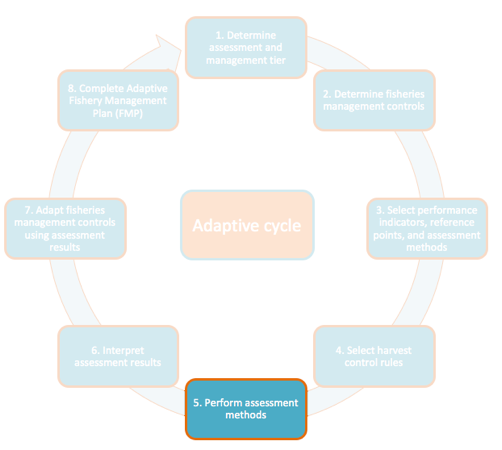
\includegraphics{myMediaFolder/media/Step5.png}
\caption{\label{fig:Step5}Step 5}
\end{figure}

During this step, you will use your data to calculate performance
indicators using the chosen assessment methods. Refer to the assessment
method descriptions under \protect\hyperlink{Step3}{Step 3} for detailed
descriptions of the assessment methods. To do the calculations, you may
use the AFAM Toolkit dashboard.

The dashboard includes data templates you may fill out using your own
data to ensure all data are properly formatted for analysis.
Alternatively, the dashboard also specifies the necessary columns for
all types of data input, so you could also simply make sure your data
has all necessary column names. Importantly, all column names must match
\emph{exactly} what is specified in the dashboard.

The dashboard currently comes pre-loaded with the necessary life history
information for many species commonly found in the Philippines,
Indonesia, Mozambique and Brazil. If your species is currently included,
you should ensure the life history parameters look reasonable for your
particular site. If they are not included, you will need to find these
parameters by looking through the literature and using resources such as
\href{www.fishbase.org}{FishBase}

If you do not have R installed on your computer, you should first
install R and R Studio on your computer using
\href{https://sfg-ucsb.github.io/fishery-manageR/}{these instructions}.

Next you will install the AFAM package onto your computer so that you
can use it in R and R Studio.

\section{Installling the dashboard from the
internet}\label{installling-the-dashboard-from-the-internet}

This is the best option and should be chosen if you have internet
connectivity. This will install the AFAM package onto your computer from
an online file sharing service (``Github''). This will ensure that your
version of the app is the most up-to-date as possible. Note that this
step requires internet connection.

If you choose this option, simply copy and paste the following code into
your R Studio console and run the code.

\begin{Shaded}
\begin{Highlighting}[]
\NormalTok{## Specify packages that are required for AFAM app. Install them if they're not installed already}
\NormalTok{list.of.packages <-}\StringTok{ }\KeywordTok{c}\NormalTok{(}\StringTok{"tidyverse"}\NormalTok{, }\StringTok{"gridExtra"}\NormalTok{, }\StringTok{"pander"}\NormalTok{, }\StringTok{"shiny"}\NormalTok{, }\StringTok{"DT"}\NormalTok{,}\StringTok{"devtools"}\NormalTok{,}\StringTok{"readxl"}\NormalTok{,}\StringTok{"stringr"}\NormalTok{,}\StringTok{"LBSPR"}\NormalTok{,}\StringTok{"TropFishR"}\NormalTok{,}\StringTok{"lubridate"}\NormalTok{,}\StringTok{"zoo"}\NormalTok{,}\StringTok{"curl"}\NormalTok{)}
\NormalTok{new.packages <-}\StringTok{ }\NormalTok{list.of.packages[}\OperatorTok{!}\NormalTok{(list.of.packages }\OperatorTok\StringTok{ }\KeywordTok{installed.packages}\NormalTok{()[,}\StringTok{"Package"}\NormalTok{])]}
\ControlFlowTok{if}\NormalTok{(}\KeywordTok{length}\NormalTok{(new.packages) }\OperatorTok{>}\StringTok{ }\DecValTok{0}\NormalTok{ ) }\KeywordTok{install.packages}\NormalTok{(new.packages)}

\NormalTok{## Load packages required for AFAM}
\KeywordTok{lapply}\NormalTok{(list.of.packages, require, }\DataTypeTok{character.only =} \OtherTok{TRUE}\NormalTok{)}

\NormalTok{## Install AFAM from Github, an online file-sharing service}
\KeywordTok{install_github}\NormalTok{(}\StringTok{"SFG-UCSB/afamAppPackage"}\NormalTok{)}
\end{Highlighting}
\end{Shaded}

\section{Installling the dashboard from a local file on your
computer}\label{installling-the-dashboard-from-a-local-file-on-your-computer}

This is the option to choose if you don't internet connectivity, but do
have a copy of the app file (this will be called something like
``afamAppPackage\_0.1.tar.gz''). This option will install the AFAM
package onto your computer using this file. Note that this may mean you
don't have the most up-to-date version of the app as possible.

If you choose this option, simply copy and paste the following code into
your R Studio console and run the code. Note that you'll need to change
the working directory to the location where you have the app file.

\begin{Shaded}
\begin{Highlighting}[]
\NormalTok{## Specify packages that are required for AFAM app. Install them if they're not installed already}
\NormalTok{list.of.packages <-}\StringTok{ }\KeywordTok{c}\NormalTok{(}\StringTok{"tidyverse"}\NormalTok{, }\StringTok{"gridExtra"}\NormalTok{, }\StringTok{"pander"}\NormalTok{, }\StringTok{"shiny"}\NormalTok{, }\StringTok{"DT"}\NormalTok{,}\StringTok{"devtools"}\NormalTok{,}\StringTok{"readxl"}\NormalTok{,}\StringTok{"stringr"}\NormalTok{,}\StringTok{"LBSPR"}\NormalTok{,}\StringTok{"TropFishR"}\NormalTok{,}\StringTok{"lubridate"}\NormalTok{,}\StringTok{"zoo"}\NormalTok{,}\StringTok{"curl"}\NormalTok{)}
\NormalTok{new.packages <-}\StringTok{ }\NormalTok{list.of.packages[}\OperatorTok{!}\NormalTok{(list.of.packages }\OperatorTok\StringTok{ }\KeywordTok{installed.packages}\NormalTok{()[,}\StringTok{"Package"}\NormalTok{])]}
\ControlFlowTok{if}\NormalTok{(}\KeywordTok{length}\NormalTok{(new.packages) }\OperatorTok{>}\StringTok{ }\DecValTok{0}\NormalTok{ ) }\KeywordTok{install.packages}\NormalTok{(new.packages)}

\NormalTok{## Load packages required for AFAM}
\KeywordTok{lapply}\NormalTok{(list.of.packages, require, }\DataTypeTok{character.only =} \OtherTok{TRUE}\NormalTok{)}

\NormalTok{## Set your working directory to where the AFAM app file is located. Note that you'll need to change this to match the actual directory on your computer}
\KeywordTok{setwd}\NormalTok{(}\StringTok{"/Users/gmcdonald/github/afamAppPackage"}\NormalTok{)}
\NormalTok{## Install AFAM from your local file}
\KeywordTok{install.packages}\NormalTok{(}\StringTok{"afamAppPackage_0.1.tar.gz"}\NormalTok{, }\DataTypeTok{repos =} \OtherTok{NULL}\NormalTok{, }\DataTypeTok{type=}\StringTok{"source"}\NormalTok{)}
\end{Highlighting}
\end{Shaded}

\section{Running the AFAM Toolkit Dashboard (does not require
internet)}\label{running-the-afam-toolkit-dashboard-does-not-require-internet}

You now have the AFAM App Package installed on your computer! To use it,
simply load the package, and run the app. You may copy and paste the
following code into your R Studio console. Note that once the package is
installed during the step above, you no longer need internet
connectivity to run the app!

\begin{Shaded}
\begin{Highlighting}[]
\NormalTok{## load Shiny package}
\KeywordTok{library}\NormalTok{(shiny)}
\NormalTok{## Load AFAM Package}
\KeywordTok{library}\NormalTok{(afamAppPackage)}

\NormalTok{## Run AFAM App}
\KeywordTok{runAFAM}\NormalTok{()}
\end{Highlighting}
\end{Shaded}

```

\hypertarget{Step6}{\chapter{Step 6 -- Interpret assessment
results}\label{Step6}}

\emph{What is the current status of the fishery?}

\begin{figure}
\centering
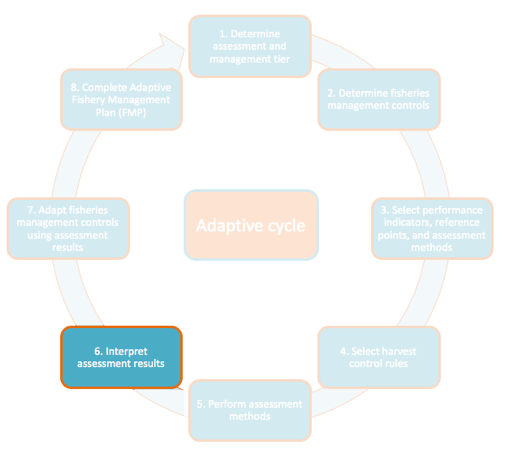
\includegraphics{myMediaFolder/media/Step6.png}
\caption{\label{fig:Step6}Step 6}
\end{figure}

\section{Step 6a - Determine the Most Likely Possible Interpretation for
Each Performance
Indicator}\label{step-6a---determine-the-most-likely-possible-interpretation-for-each-performance-indicator}

After assessment methods have been completed, use your harvest control
rule table to determine the possible interpretation and management
implication for each performance indicator using the following steps:

\begin{enumerate}
\def\labelenumi{\alph{enumi})}
\item
  Using your assessment results \protect\hyperlink{Step5}{Step 5}, use
  your harvest control rule table to look up the most likely
  interpretation from the choices provided in the ``Possible
  Interpretation'' column.
\item
  Once the most likely possible interpretation has been chosen,
  determine the management implication by locating the colored circle
  traffic light in the ``Management Implication column''
\end{enumerate}

\section{Step 6b -- Verify Assessment Result and
Interpretation}\label{step-6b-verify-assessment-result-and-interpretation}

Verify the assessment result using the following steps:

\begin{enumerate}
\def\labelenumi{\arabic{enumi}.}
\item
  Double-check calculations by reviewing the assessment calculations.
\item
  Double-check that each assessment performed was stratified to the
  spatial extent of the fishery; for example, run analyses for each gear
  type, boat type, and/or fishing area.
\item
  Double-check that reference points are appropriate for your fishery
  using available literature, expert opinion, and local ecological
  knowledge
\item
  Review fishery-dependent sampling protocol; assess whether or not the
  spatial extent of the fishery-dependent survey overlaps with known or
  assumed distribution of fish population as well as fishing effort and
  gear type. If the sampling protocol, fish population, and fishing
  effort do not overlap, there may be biases in the assessment results
  that should be considering in your interpretation.
\item
  Review fishery-independent sampling protocol; assess whether or not
  the spatial extent of the fishery-independent survey overlaps with
  known or assumed distribution of fish population as well as fishing
  effort. If the sampling protocol, fish population, and fishing effort
  do not overlap, there may be biases in the assessment results that
  should be considering in your interpretation.
\item
  Examine any effort metrics to determine if they are consistent with
  your interpretation
\item
  Groundtruth assessment result and interpretation with community.
  Consult with local experts to determine if the assessment results
  align with their knowledge of the fishery (fishers, middlemen, village
  elders, academic research groups, etc.) Often, assessment results can
  be counterintuitive, and multiple performance indicators may be
  conflicting in their message. Fishers can be especially helpful in
  interpreting performance indicators that seem counter-intuitive but
  can be explained by fishermen behavior -- for example, if
  fished:unfished density ratio is down but catch and CPUE are up, the
  fishermen might say that although fish abundance seems low (low
  fished:unfished density ratio) prices were high that season and the
  weather was good, resulting in better targeting (higher CPUE) and
  higher catches. This process can either take place in a focus group
  discussion or structured interviews with key stakeholders. Through
  this process, try to arrive at a consistent interpretation.
\item
  If trends persist, each performance indicator points towards a
  consistent interpretation, and if the community agrees with the
  interpretation, proceed to \protect\hyperlink{Step7}{Step 7}
\item
  In situations where conflicting indicators cannot be rectified, or if
  the community cannot corroborate the assessment results, additional
  community outreach or other forms of social marketing may be necessary
  to arrive at consensus. *It's important that all stakeholders are
  comfortable and confident with the assessment interpretation because
  it will be used to trigger a harvest control rule in
  \protect\hyperlink{Step7}{Step 7}.
\end{enumerate}

\hypertarget{Step7}{\chapter{Step 7 -- Adjust Fisheries Management
Controls Using Defined Harvest Control Rules}\label{Step7}}

\emph{How should I adjust fisheries management controls based on my
assessment results and interpretation?}

\begin{figure}
\centering
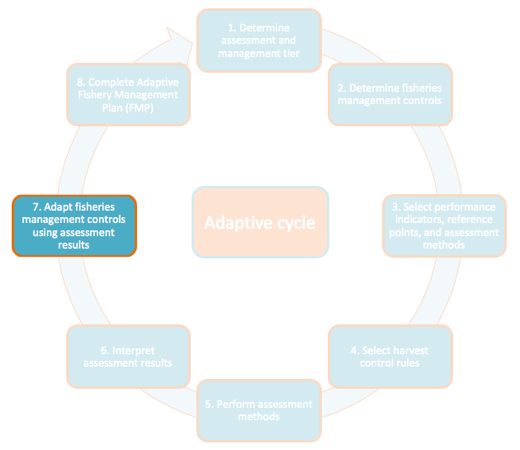
\includegraphics{myMediaFolder/media/Step7.png}
\caption{\label{fig:Step7}Step 7}
\end{figure}

After interpreting and verifying the assessment results, implement the
appropriate HCR defined in \protect\hyperlink{Step4}{Step 4}. Depending
on the severity of the HCR and likely community reaction, it may be
necessary to conduct additional community outreach or other social
marketing activities to ensure buy-in and compliance. For example, if a
limit reference point is reached and the fishery for a particular
species must be closed, this will likely require significant community
outreach.

\hypertarget{Step8}{\chapter{Step 8 -- Complete Your Fishery Management
Plan}\label{Step8}}

\emph{How do I take the outputs of the AFAM toolkit to create a concrete
Fishery Management Plan?}

\begin{figure}
\centering
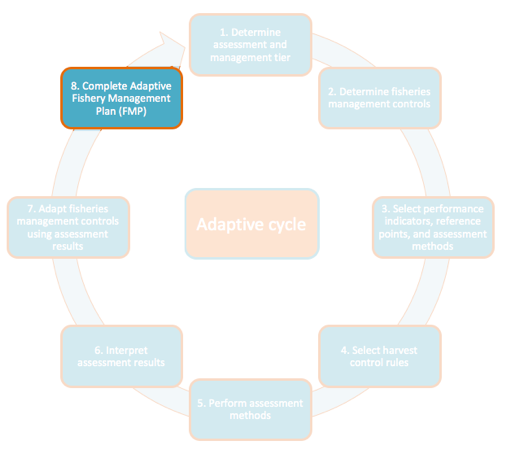
\includegraphics{myMediaFolder/media/Step8.png}
\caption{\label{fig:Step8}Step 8}
\end{figure}

We have provided a template Fishery Management Plan below. To complete
this template, we recommend you use the outputs of the AFAM Dashboard.
We recommend you complete a fishery management plan for each species to
be managed. Note that the template provided here may need to be adapted
to better suit your regional context.

\section{Fishery Management Plan
Template}\label{fishery-management-plan-template}

\begin{itemize}
\item
  \textbf{Fishery Overview:}

  \begin{itemize}
  \item
    \textbf{Location of the Fishery}: Country, state, city, management
    zone (if applicable).
  \item
    \textbf{History}: Provide a brief history of the fishery.
  \item
    \textbf{Type(s) of Fishery}: Commercial, recreational, etc. and
    whether near shore, off shore, or mixed.
  \item
    \textbf{Participants}: Number of fishers, number of vessels, number
    of communities (if applicable), and spatial distribution of
    participants/ communities.
  \item
    \textbf{Fishery Characteristics}: Describe the gear types utilized
    in the fishery (i.e.~fixed gear, mobile gear, etc), including
    numbers for each if possible, as well as the general timeframe
    (i.e.~season) of when the fishery occurs.
  \item
    \textbf{Management Characteristics}: Type of method currently used
    to manage the fishery (i.e.~seasons, catch limits, size limits,
    effort limits, etc.). Also describe the general management
    decision-making process.
  \item
    \textbf{Governance}: Briefly describe key legislation and
    regulations, as well as types of committees and/or legislative land
    claims which are part of the decision making process (based on
    zones, areas, regions, international considerations).
  \item
    \textbf{Economic, Social, and Cultural Importance of the Fishery}:
    Provide a brief overview of economic conditions and social, cultural
    and economic issues.
  \item
    \textbf{Species Characteristics}: Provide a brief overview outlining
    the main biological characteristics of the species with emphasis on
    the aspects which impact on management of the species. Factors to be
    covered include range (both globally and locally), populations/stock
    structure, habitat requirements (including key location where
    applicable), migration routes and reproductive characteristics
    (i.e.~season, behavior, fecundity, growth rates, spawning grounds).
  \item
    \textbf{Ecosystem Interactions}: Briefly describe interactions with
    other species and the physical environment. Where the information is
    available briefly describe the effect of climate regime changes on
    stock status, particularly recruitment and stock productivity.
  \end{itemize}
\item
  \textbf{Fisheries Objectives and Challenges:}
\end{itemize}

\textbf{\emph{You may use the outputs of the FLAGS toolkit to help
complete this section.}}

\begin{itemize}
\item
  \textbf{Management Objectives}: Clearly state long-term objectives for
  fishery management under the following potential headings:

  \begin{itemize}
  \item
    \textbf{Yield/ Economic}
  \item
    \textbf{Stock Conservation}
  \item
    \textbf{Ecosystem }
  \item
    \textbf{Social and Cultural}
  \item
    \textbf{Compliance}

    \begin{itemize}
    \tightlist
    \item
      For each long-term objective, outline short-term objectives
      specific for the duration of the plan.
    \end{itemize}
  \end{itemize}
\item
  \textbf{List all Trade-Offs Associated with these Objectives}: Provide
  a brief explanation of which objectives conflict with each other, such
  that one objective may have to be sacrificed to achieve another. Where
  possible, discuss potential management modifications that may lessen
  these trade-offs.
\item
  \textbf{Current Management Issues}: Provide an overview of current
  issues in the fishery, including those related to the target species,
  as well as by-catch and ecosystem concerns. Potential examples of
  management issues include:

  \begin{itemize}
  \item
    \textbf{\emph{Fisheries Issues}} such as conflicts between gear
    sectors, catch monitoring, by-catch problems and other resource user
    issues.
  \item
    \textbf{\emph{Depleted Species Concerns}}, including species listed
    under CITES, and/ or any local endangered/threatened species
    legislation. Reference existing recovery strategies/management plans
    where appropriate.
  \item
    \textbf{\emph{Oceans and Habitat Considerations}}, including habitat
    impacts and discussions of ecologically significant areas that have
    been identified and documented within the geographic range of the
    fishery (including marine protected areas (MPAs) or no-take zones.
    Where information is available on the effect of climate regime
    change on stock status, it should be considered when developing
    harvest decision rules and other management measures. Any management
    measures in place to control aquatic invasive species should also be
    included.
  \item
    \textbf{\emph{Gear Impacts}}, including losses and resulting
    impacts.
  \item
    \textbf{\emph{International Issues}}
  \end{itemize}
\end{itemize}

\begin{itemize}
\tightlist
\item
  \textbf{Science and Traditional Knowledge:}
\end{itemize}

\textbf{\emph{You may use your Site Level Research Plan, the Global
Monitoring \& Evaluation Plan, and the Data Collection Manual to help
you complete this section.}}

\begin{itemize}
\item
  **Available \url{Data:**} Provide brief overview of all available
  data, with references to sources.
\item
  \textbf{Data Collection:} Provide a brief overview of the data
  collection process for the stock(s), including types of data sources
  utilized (i.e.~research vessel trawl surveys, tagging, index
  fisheries, CPUE, landing statistics, sentinel fisheries, etc.) and
  frequency of assessment.
\item
  \textbf{Traditional Knowledge:} Provide brief overview of all
  traditional/ local knowledge.
\item
  \textbf{Research:} Provide a brief overview of research projects being
  conducted during the period of the plan and their purpose. Also
  include any research needs not currently being addressed. Consider not
  just the target species, but also research on associated by-catch and
  habitat.
\item
  \textbf{Precautionary Approach (PA)}: Where available, provide a brief
  overview of any PA references established for this resource, including
  removal references, limit reference points, and upper stock reference
  points.
\end{itemize}

\begin{itemize}
\item
  \textbf{Adaptive Assessment and Management:}

  Provide a brief overview of the \textbf{Adaptive Fisheries Assessment
  and Management Plan}, including data sources, design of data
  collection and sampling programs, timeline for completion of new/
  updated assessments (e.g., yearly), and performance indicators to be
  evaluated.

  \begin{itemize}
  \item
    \textbf{Step 1: Assessment and management tier chosen}.

    \begin{itemize}
    \item
      \textbf{Data sources: }

      \begin{itemize}
      \tightlist
      \item
        \textbf{Tier:}
      \end{itemize}
    \end{itemize}
  \item
    \textbf{Step 2: Fisheries Management Controls}

    \begin{itemize}
    \tightlist
    \item
      \textbf{Species Productivity score:}
    \end{itemize}
  \item
    \textbf{Step 3:} List \textbf{performance indicators, reference
    points, and assessment methods} chosen.

    \begin{itemize}
    \item
      \textbf{Performance indicators: }

      \begin{itemize}
      \item
        \textbf{Data Streams:}
      \item
        \textbf{Target RP}
      \item
        \textbf{Limit RP}
      \item
        \textbf{Assessment method}
      \item
        \textbf{Results/Reasoning:}
      \end{itemize}
    \item
      \textbf{Performance indicators: }

      \begin{itemize}
      \item
        \textbf{Data Streams:}
      \item
        \textbf{Target RP}
      \item
        \textbf{Limit RP}
      \item
        \textbf{Assessment method}
      \item
        \textbf{Results/Reasoning:}
      \end{itemize}
    \item
      \textbf{Performance indicators (if applicable): }

      \begin{itemize}
      \item
        \textbf{Data Streams:}
      \item
        \textbf{Target RP}
      \item
        \textbf{Limit RP}
      \item
        \textbf{Assessment method}
      \item
        \textbf{Results/Reasoning:}
      \end{itemize}
    \item
      \textbf{Performance indicators (if applicable): }

      \begin{itemize}
      \item
        \textbf{Data Streams:}
      \item
        \textbf{Target RP}
      \item
        \textbf{Limit RP}
      \item
        \textbf{Assessment method}
      \item
        \textbf{Results/Reasoning:}
      \end{itemize}
    \end{itemize}
  \item
    \textbf{Step 4: Define Harvest Control Rules}

    \begin{itemize}
    \item
      \textbf{First performance indicators: }

      \begin{itemize}
      \item
        \textbf{Assessment Result:}
      \item
        \textbf{Interpretation (s):}
      \item
        \textbf{Management Implications:}
      \item
        \textbf{HCR suggested in literature:}
      \item
        \textbf{Implemented HCR:}
      \end{itemize}
    \item
      \textbf{Second performance indicators (if applicable): }

      \begin{itemize}
      \item
        \textbf{Assessment Result:}
      \item
        \textbf{Interpretation (s):}
      \item
        \textbf{Management Implications:}
      \item
        \textbf{HCR suggested in literature:}
      \item
        \textbf{Implemented HCR:}
      \end{itemize}
    \item
      \textbf{Third performance indicators (if applicable): }

      \begin{itemize}
      \item
        \textbf{Assessment Result:}
      \item
        \textbf{Interpretation (s):}
      \item
        \textbf{Management Implications:}
      \item
        \textbf{HCR suggested in literature:}
      \item
        \textbf{Implemented HCR:}
      \end{itemize}
    \item
      \textbf{Fourth performance indicators (if applicable): }

      \begin{itemize}
      \item
        \textbf{Assessment Result:}
      \item
        \textbf{Interpretation (s):}
      \item
        \textbf{Management Implications:}
      \item
        \textbf{HCR suggested in literature:}
      \item
        \textbf{Implemented HCR:}
      \end{itemize}
    \item
      \textbf{Fifth performance indicators (if applicable): }

      \begin{itemize}
      \item
        \textbf{Assessment Result:}
      \item
        \textbf{Interpretation (s):}
      \item
        \textbf{Management Implications:}
      \item
        \textbf{HCR suggested in literature:}
      \item
        \textbf{Implemented HCR:}
      \end{itemize}
    \end{itemize}
  \item
    \textbf{Step 5:} Interpret assessment results.

    \begin{itemize}
    \item
      \textbf{First method applied: }

      \begin{itemize}
      \item
        \textbf{Results:}
      \item
        \textbf{Interpretations:}
      \end{itemize}
    \item
      \textbf{Second method applied (if applicable):}

      \begin{itemize}
      \item
        \textbf{Results:}
      \item
        \textbf{Interpretations:}
      \end{itemize}
    \item
      \textbf{Third method applied (if applicable):}

      \begin{itemize}
      \item
        \textbf{Results:}
      \item
        \textbf{Interpretations:}
      \end{itemize}
    \item
      \textbf{Fourth method applied (if applicable):}

      \begin{itemize}
      \item
        \textbf{Results}
      \item
        \textbf{Interpretations:}
      \end{itemize}
    \item
      \textbf{Fifth method applied (if applicable):}

      \begin{itemize}
      \item
        \textbf{Results}
      \item
        \textbf{Interpretations:}
      \end{itemize}
    \end{itemize}
  \item
    \textbf{Step 6: Adjust fisheries management controls using defined
    harvest control rules }

    \begin{itemize}
    \tightlist
    \item
      \textbf{Triggered Harvest Control Rules:}
    \end{itemize}
  \end{itemize}
\item
  \textbf{Additional Management Measures for the Duration of the Plan: }

  \begin{itemize}
  \item
    \textbf{Management measures:} Specify if plan is for a single year
    or multiple years. In the latter case, identify expected management
    changes in each successive year. Where relevant, include any
    mandatory financial arrangements required with fish harvesters and
    other stakeholders.
  \item
    \textbf{Monitoring measures} may include:

    \begin{itemize}
    \item
      \textbf{\emph{Observer coverage }}
    \item
      \textbf{\emph{Dockside monitoring}}
    \item
      \textbf{\emph{Logbooks }}
    \item
      \textbf{\emph{Hailing}}
    \item
      \textbf{\emph{Electronic vessel monitoring systems}}
    \item
      \textbf{\emph{Etc.}}
    \end{itemize}
  \item
    \textbf{Enforcement measures} may include:

    \begin{itemize}
    \item
      \textbf{\emph{Fines}}
    \item
      \textbf{\emph{Sanctions}}
    \item
      \textbf{\emph{Quota revocations}}
    \item
      \textbf{\emph{Vessel suspensions}}
    \item
      \textbf{\emph{Criminal }}
    \end{itemize}
  \end{itemize}
\item
  \textbf{Stock Scenarios}: Briefly describe expected stock prospects
  (i.e.~trends) for period of the plan, and beyond, if available.
\item
  \textbf{Management Plan Performance Review}: Outline indicators that
  will be used to determine if the plan objectives are met. Where
  applicable, include results of previous year's review.
\end{itemize}

\hypertarget{Glossary}{\chapter{Glossary}\label{Glossary}}

\textbf{Assessment Method} - The method for using raw data to calculate
performance indicators.

\textbf{Boat intercept / landing site surveys -} Baseline boat intercept
and landing site surveys are meant to gather information on catch and
effort in order to establish a baseline catch-per-unit-effort (CPUE)
indicator. These surveys can be useful in establishing baseline CPUE in
areas where individual catch reporting systems are not yet in place.
This information should be broken down by species and gear type. Boat
intercepts involve at-sea intercepts of fishing boats, and are typically
conducted in areas where fish is landed at a large number of sites.
Landing site surveys are typically conducted where fish is landed at a
relatively small number of sites. To establish baseline CPUE we
recommend landing site surveys. The information from these surveys can
be used to inform fisheries management as well as impact monitoring over
time as it relates to productive and profitable fisheries. Refer to the
FF Data Collection Manual for more details.

\textbf{Bycatch -} A species or individual fish that is caught
unintentionally. This term may refer to any landings that do not contain
the species that as targeted or it may refer to a certain size class or
sex of a species that was unintentionally landed. For example, a
juvenile fish landed that is under the specified size limit would be
considered bycatch.

\textbf{Control} -- See \textbf{Fisheries Management Control (FMC)}

\textbf{Discard Mortality --} How likely a fish is to die after it has
been landed and released (and not counted as part of total harvest).
Discard mortality rates will vary with different fishing gears and
between species.

\textbf{Destructive Fishing Methods -} These are unselective fishing
methods that result in high discard mortality and are defined in this
tool as: dynamite fishing, fishing with chemicals or harmful substances,
the use of nets with fine mesh.

\textbf{Experimental Fishing --} Fishery-independent experimental
fishing surveys gather ecological information on the finfish of a
particular area. This information can include biomass and species
richness. Individuals who are trained in local species and ecology
conduct these surveys. Local fishers can be employed to use a specific
gear in specified sampling locations and at specified sampling times.
This type of information can be used to better understand the health of
a particular ecosystem and inform fisheries management, and is also
important for monitoring impact as it relates to ecosystem conservation
and resilience.

\textbf{Fisheries Management Control (FMC) --} Fisheries management
controls are measures that managers may implement to limit fishing
activity with the main objective of either limiting fishing mortality or
protecting key biological or ecological features of the fishery.
Definitions of recommended FMCs are provided in Table A2.1.

\textbf{Fishery-dependent species length composition survey -} The
survey will gather individual fish length measurements of key target
species in order to construct length frequency compositions of those
species. A fishery dependent length composition indicates how many fish
of each size are being caught in the fishery. This information can
inform how well the fishery is doing through key indicators such as
average length or fishing mortality. This can be used to inform
fisheries management as well as impact monitoring over time as it
relates to productive fisheries. Refer to the FF Data Collection Manual
for more details.

\textbf{Harvest Control Rule (HCR) -} A harvest control rule helps
stakeholders to compare performance indicators with reference points and
adjust fisheries management controls accordingly. In other words, a
harvest control rule is a plan for pre-agreed management actions as a
function of variables related to the status of stock in question.

\textbf{Highgrading -} When fishermen selectively only keep harvested
fish that are the highest quality (ex. The largest) and discard the
lower quality catch. Typically occurs when only a limited number of fish
can be harvested.

\textbf{Individual Catch Reporting System -} This is the system that
will gather catch and effort data for the fishery as well as price and
cost data necessary for computing profit. This information should be
broken down by species and gear type, and in ideal circumstances would
cover all landings and effort of all fishers. Additionally, fishers
should indicate the location where their catch was caught if possible.
Ideally, all fishers report their catch daily in log books. Refer to the
FF Data Collection Manual for more details.

\textbf{Limit Reference Point (LRP)} - A numerical value that indicates
that the status of a stock is unacceptable (e.g.~overfished).

\textbf{Megaspawner -} Old, large fish that contribute a
disproportionately significant amount of reproductive potential of the
stock

\textbf{Performance Indicators -} A numerical value (or range of values)
that is used to determine the current state of the fishery. Performance
indicators can be examined over time, space or against a predetermined
reference point\textbf{.}

\textbf{`Race to Fish'-} Occurs when fishermen are fishing against a
single quota or for a limited time frame. Fishermen begin to race each
other to catch as many fish as possible before the fishery is closed.
This often leads to fishermen investing in more efficient gear, using
too many gears, fishing during unsafe weather conditions, higher bycatch
rates, and reduced value of catch due to market floods.

\textbf{Reference Point:} A reference point is what your performance
indicator is compared with when assessing the performance of your
fishery. By comparing your performance indicator on an annual with a
pre-determined reference point, you can assess how your fishery is
doing. There are two types of references points: limit reference points
(LRPs) and target reference points (TRPs).

\textbf{Target Reference Point (TRP) -} A numerical value (or range of
values) that indicates that the status of a stock is at a desirable
level, often times management is geared towards achieving or maintaining
this target.

\textbf{Underwater Visual Survey --} Fishery-independent underwater
visual surveys gather ecological information on the finfish,
invertebrate, and benthic habitat composition of a particular area. This
information can include biomass, species richness, and coral and
macroalgal cover. Individuals who are trained in local species and
ecology conduct these surveys. SCUBA or snorkeling is used in order to
conduct linear transects, quadrats, patch reef surveys, manta tows, or
roaming surveys. This type of information can be used to better
understand the health of a particular ecosystem and inform fisheries
management, and is also important for monitoring impact as it relates to
ecosystem conservation and resilience.

\chapter{References}\label{references}

Ault, J., Smith, S., \& Bohnsack, J. (2005). Evaluation of average
length as an estimator of exploitation status for the Florida coral-reef
fish community. ICES Journal of Marine Science, 62(3), 417--423.
\url{doi:10.1016/j.icesjms.2004.12.001}

Babcock, E. a., \& MacCall, A. D. (2011). How useful is the ratio of
fish density outside versus inside no-take marine reserves as a metric
for fishery management control rules? Canadian Journal of Fisheries and
Aquatic Sciences, 68(2), 343--359. \url{doi:10.1139/F10-146}

Beverton, R. J. H., and Holt, S. J. (1959). A review of the lifespans
and mortality of fish in nature and the relation to growth and other
physiological characteristics. Ciba Foundation Colloquium on Ageing, 5:
142--177.

Cope, Jason M., and André E. Punt. ``Length‐Based Reference Points for
Data‐Limited Situations: Applications and Restrictions.'' Marine and
Coastal Fisheries 1.1 (2009): 169-186.
\url{http://onlinelibrary.wiley.com/doi/10.1577/C08-025.1/full}.

Ehrhardt, N.M. \& Ault, J.S. (1992). Analysis of two length-based
mortality models applied to bounded catch length frequencies. Trans. Am.
Fish. Soc., 121, 115-

\begin{enumerate}
\def\labelenumi{\arabic{enumi}.}
\setcounter{enumi}{121}
\item
\end{enumerate}

Froese, R. (2004). Keep it simple: three indicators to deal with
overfishing. Fish and Fisheries, 5, 86--91.

Harford, W.J., Gedamke, T., Babcock, E.A., Carcamo, R., McDonald, G., \&
Wilson, J.R. Management strategy evaluation of a multi-indicator
adaptive framework for data-limited fisheries management (2016).
Bulletin of Marine Science. \url{https://doi.org/10.5343/bms.2016.1025}.

Hordyk, A., Ono, K., Valencia, S., Loneragan, N., \& Prince, J. (2014).
A novel length-based empirical estimation method of spawning potential
ratio (SPR), and tests of its performance, for small-scale, data-poor
fisheries. ICES Journal of Marine Science.
\url{doi:10.1093/icesjms/fsu004}

Karr, K. A., Fujita, R., Halpern, B. S., Kappel, C. V., Crowder, L.,
Selkoe, K. A., P. M. Alcolado, and D. Rader (2014). Thresholds in
Caribbean coral reefs: Implications for ecosystem-based fishery
management. Journal of Applied Ecology.
\url{doi:10.1111/1365-2664.12388}

McClanahan, T. R., Graham, N. a. J., MacNeil, M. A., Muthiga, N. a.,
Cinner, J. E., Bruggemann, J. H., \& Wilson, S. K. (2011). Critical
thresholds and tangible targets for ecosystem-based management of coral
reef fisheries. Proceedings of the National Academy of Sciences of the
United States of America, 108(41), 17230--3.
\url{doi:10.1073/pnas.1106861108} McDonald et al., 2018. An adaptive
assessment and management toolkit for data-limited fisheries. Ocean and
Coastal Management, 152 (2018), pp.~100-119.
\url{https://doi.org/10.1016/j.ocecoaman.2017.11.015}

McDonald et al., 2018. An adaptive assessment and management toolkit for
data-limited fisheries. Ocean and Coastal Management, 152 (2018).
\url{https://doi.org/10.1016/j.ocecoaman.2017.11.015}

McDonald G., Harford B., Arrivillaga A., Babcock E.A., Carcamo R., Foley
J., Fujita R., Gedamke T., Gibson J., Karr K., Robinson J., Wilson J.
(2016) An indicator-based adaptive management framework and its
application to data-limited fisheries in Belize. Marine Policy.
\url{http://doi.org/10.1016/j.marpol.2016.11.027}

McDonald, G., Carcam, R., Fujita, R., Gedamke, T., Karr, K., Wilson, J.
A multi-indicator framework for adaptive management of data-limited
nearshore fisheries: A case study from Belize (2014). Proceedings of the
67\textsuperscript{th} Annual Gulf and Caribbean Fisheries Institute,
Christ Church, Barbados, November 2014.

Prince, J., Hordyk, A., Valencia, S. R., Loneragan, N., \& Sainsbury, K.
(2014). Revisiting the concept of Beverton -Holt life-history invariants
with the aim of informing data-poor fisheries assessment. ICES Journal
of Marine Science, (1959). \url{doi:10.1093/icesjms/fsu011}

Robson, D. and G. Chapman. 1961. Catch Curves and Mortality Rates.
Transactions of the American Fisheries Society 90 (2): 1810189.

\chapter{AFAM Toolkit Worksheet}\label{afam-toolkit-worksheet}

The AFAM Toolkit dashboard will keep track of all of your steps and
automatically generate a report once you've complete all steps. However,
you may also wish to keep track of the outputs from each step on a hard
copy piece of paper, especially since the dashboard does not currently
allow you to save your work.

As your work through each step, fill out the following tables.

\textbf{Step 1 -- Determine assessment and management tiertermine
assessment and management tier}

\emph{Step 1 outputs -- Data Inventory}

\begin{tabular}{l|l|l|l}
\hline
Minimum Required Data & Needed? & Available? & Years of data\\
\hline
Qualitative characterization of the fishery & Required &  & \\
\hline
List of prioritized species for management & Required &  & \\
\hline
List of prioritized goals for management & Required &  & \\
\hline
Landings, effort, and CPUE of key target species & Optional &  & \\
\hline
Length composition data of key target species & Optional &  & \\
\hline
Density ratio from UVC (key target species) & Optional &  & \\
\hline
Biomass ratio from UVC (aggregated across species) & Optional &  & \\
\hline
\end{tabular}

\emph{Step 1 outputs -- Assessment and Management Tier}

\begin{tabular}{l|l}
\hline
  & Response\\
\hline
What is your assessment and management tier? & \\
\hline
Notes & \\
\hline
\end{tabular}

\textbf{Step 2 -- Determine appropriate Fisheries Management Controls}

\emph{Step 2 outputs -- Existing fisheries management controls (FMCs)}

\begin{tabular}{l|l|l|l}
\hline
  & Existing FMC 1 & Existing FMC 2 & Existing FMC 3\\
\hline
Name of Existing FMC &  &  & \\
\hline
Who introduced this FMC? Who implements this FMC? &  &  & \\
\hline
Resources required for implementation &  &  & \\
\hline
Level of compliance &  &  & \\
\hline
Community Attitude towards FMC &  &  & \\
\hline
Is the FMC effective in meeting management objectives? &  &  & \\
\hline
Other implementation pro/cons &  &  & \\
\hline
Notes &  &  & \\
\hline
\end{tabular}

\emph{Step 2 outputs -- Potential new fisheries management controls
(FMCs)}

\begin{tabular}{l|l|l|l}
\hline
Question & New FMC 1 & New FMC 2 & New FMC 3\\
\hline
Name of potential new FMC &  &  & \\
\hline
Possible Implications (positive or negative) &  &  & \\
\hline
\end{tabular}

\textbf{Step 3 -- Select performance indicators, reference points, and
assessment methods}

\emph{Step 3 outputs} Note: We generally recommend using 3 performance
indicators, from 3 independent data sources if possible.

\begin{tabular}{l|l|l|l}
\hline
  & PI 1 & PI 2 & PI 3\\
\hline
Performance Indicator Name &  &  & \\
\hline
Data source &  &  & \\
\hline
Target Reference Point (TRP) &  &  & \\
\hline
Limit Reference Point (LRP) &  &  & \\
\hline
Notes &  &  & \\
\hline
\end{tabular}

\textbf{Step 4 -- Define Harvest Control Rules} \emph{Step 4 outputs}

\begin{tabular}{r|l|l|l|l|l}
\hline
Scenario & PI 1 Stoplight & PI 2 Stoplight & PI 3 Stoplight & Interpretation & Management Response\\
\hline
1 &  &  &  &  & \\
\hline
2 &  &  &  &  & \\
\hline
3 &  &  &  &  & \\
\hline
4 &  &  &  &  & \\
\hline
5 &  &  &  &  & \\
\hline
6 &  &  &  &  & \\
\hline
7 &  &  &  &  & \\
\hline
8 &  &  &  &  & \\
\hline
\end{tabular}

\textbf{Step 5 - Perform assessment methods} \emph{Step 5 outputs}

\begin{tabular}{l|l|l|l}
\hline
  & PI 1 & PI 2 & PI 3\\
\hline
PI Name &  &  & \\
\hline
PI Value &  &  & \\
\hline
Notes &  &  & \\
\hline
\end{tabular}

\textbf{Step 6 -- Interpret assessment results} \emph{Step 6 outputs}

\begin{tabular}{l|l|l|l}
\hline
  & PI 1 & PI 2 & PI 3\\
\hline
PI Name &  &  & \\
\hline
PI Value &  &  & \\
\hline
TRP Value &  &  & \\
\hline
LRP Value &  &  & \\
\hline
Stoplight Result &  &  & \\
\hline
\end{tabular}

\textbf{Step 7 - Adjust fisheries management controls using defined
harvest control rules} \emph{Step 7 outputs}

\begin{tabular}{l|l}
\hline
  & Response\\
\hline
Selected management response & \\
\hline
Notes & \\
\hline
\end{tabular}

\bibliography{packages.bib,book.bib}


\end{document}
